%% GENERATED by scripts/paper/build_paper.py from docs/analysis/register/findings.yaml -- do not edit by hand;
%% rewrite the prose in main.tex or change the register / scripts/paper/paper_text.json and rebuild.

\subsection{Each operator has a personal style --- individual, not a type (supplementary analyses)}\label{sec:sup:res:personal-style}

\noindent Supplement to Section~\ref{sec:res:personal-style}.

\subsubsection{After one session we can recognise a person's style in the next}\label{sec:res:personal-style:fingerprint}

\noindent \passtag{numbers only}

\noindent \regtext{Each session is summarised as ten habits (below). Comparing everyone's session-1 profile with everyone's session-2 profile, the closest match is far more often the \textbf{same person} than chance allows. It is a ``near neighbour'' result, not exact identification: the own session is the single closest match for 7 of 33 people (chance: 1), but in the closest three for 41\% (chance 9\%), and on average ranks 8th of 33 (chance 17th). It survives taking the reliance axis out --- so the style is more than ``how much do you lean on the assistants''. In the matrix, every row is one person's session 1, every column a session 2, darker = closer; the outlined diagonal is each person against themselves.} (Figure~\ref{fig:res:personal-style:fingerprint})

\begin{figure}[H]
\centering
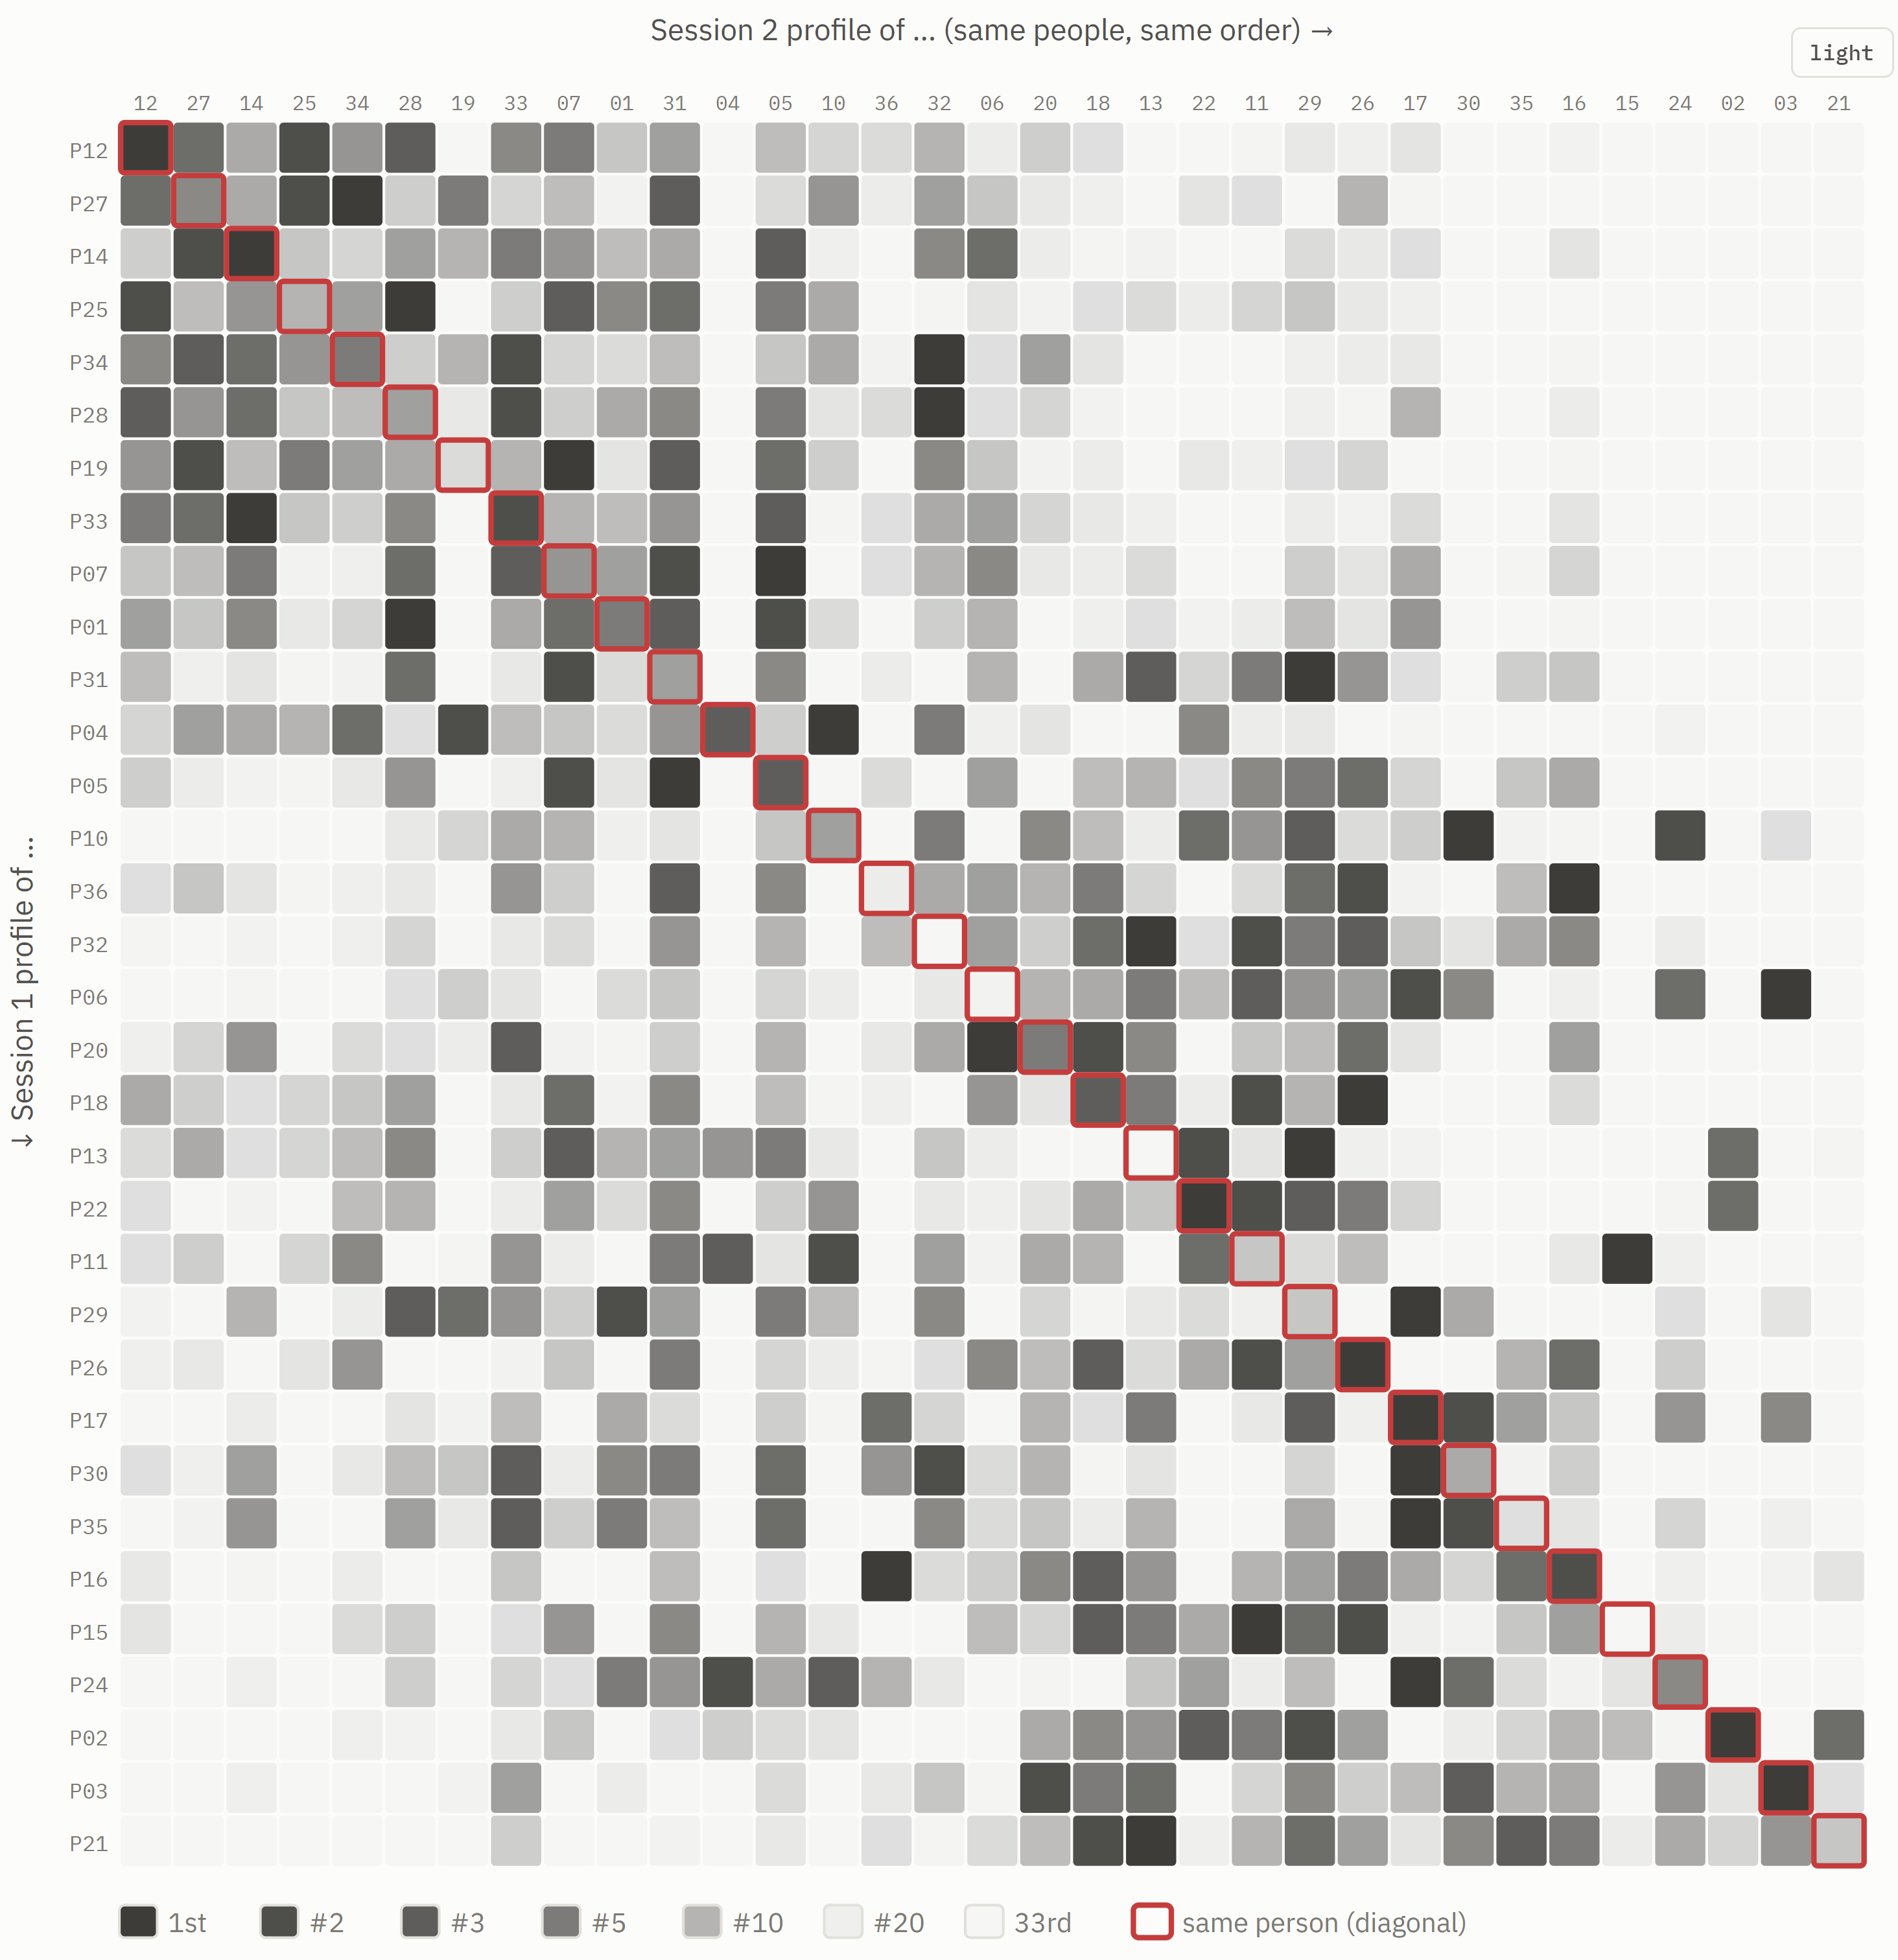
\includegraphics[width=\linewidth,height=0.55\textheight,keepaspectratio]{figs/results/f-personal-style__fingerprint__main.png}
\caption{\textbf{After one session we can recognise a person's style in the next}}
\label{fig:res:personal-style:fingerprint}
\end{figure}

\paragraph*{Key numbers.}

\begin{itemize}[leftmargin=1.2em,itemsep=1pt]

\item Own session nearest: 7 of 33 (session 1 $\rightarrow$ 2) and 5 of 33 (2 $\rightarrow$ 1); chance $\approx$ 1; permutation p < .001

\item Own session in the closest 3: 41\% vs 9\% by chance; mean rank 8.2 of 33 vs 17.0 (p < .001)

\item Reliance axis removed: 6 and 6 of 33, top-3 32\%, mean rank 10.1 (p < .001) --- the style is more than reliance

\item Reliance axis alone: 4 and 4 of 33, top-3 27\%, mean rank 11.1

\item Profile correlation with own other session: median r = .48; with other people's: median r = $-$.01; own closer for 29 of 33 (sign test p < .001)

\end{itemize}

\paragraph*{Method.} {\small Rows: 66 sessions (33 people $\times$ 2). Each session becomes a vector of ten habits: share of strategy cards taken; share of manual choices made before the cards loaded; share of cards edited; share of tactical plans where Suggest was pressed; share of Suggest plans kept unchanged; share of recovery episodes with Suggest pressed; time per strategic decision beyond the forced card delay (log); drones committed vs the Conservative card on single-type and on multi-type missions; card previews per decision. Each habit is turned into a z-score \emph{within the game played} (so a hard game does not make everyone in it look alike; a habit with no data in a session, e.g. no recoveries, is set to that game's median). For each person's session-1 vector we measure the straight-line (Euclidean) distance to all 33 session-2 vectors and rank them; ``rank 1'' means their own session 2 is the nearest. Done both ways (session 1 looking among session 2s and vice versa). The p-value comes from shuffling who-is-who in session 2 10 000 times and counting how often chance does as well. ``Reliance axis removed'': the single strongest direction of variation (PC1, see below) is subtracted from every vector first. The profile correlation r is the Pearson correlation between a person's two ten-habit vectors (1 = same shape, 0 = unrelated). Exploratory and post hoc; the permutation test is clean. People are ordered by reliance in the matrix, so neighbours look alike --- the claim is that the diagonal beats them.}

\clearpage

\subsubsection{What a personal style looks like}\label{sec:res:personal-style:profiles}

\noindent \passtag{extra: may make it in}

\noindent \regtext{Every person's ten habits in session 1 (light) and session 2 (dark). The top rows are people whose two sessions have almost the same shape (r up to .89); at the bottom are the few whose style changed (P13, P29, P32). Most people repeat themselves.} (Figure~\ref{fig:res:personal-style:profiles})

\begin{figure}[H]
\centering
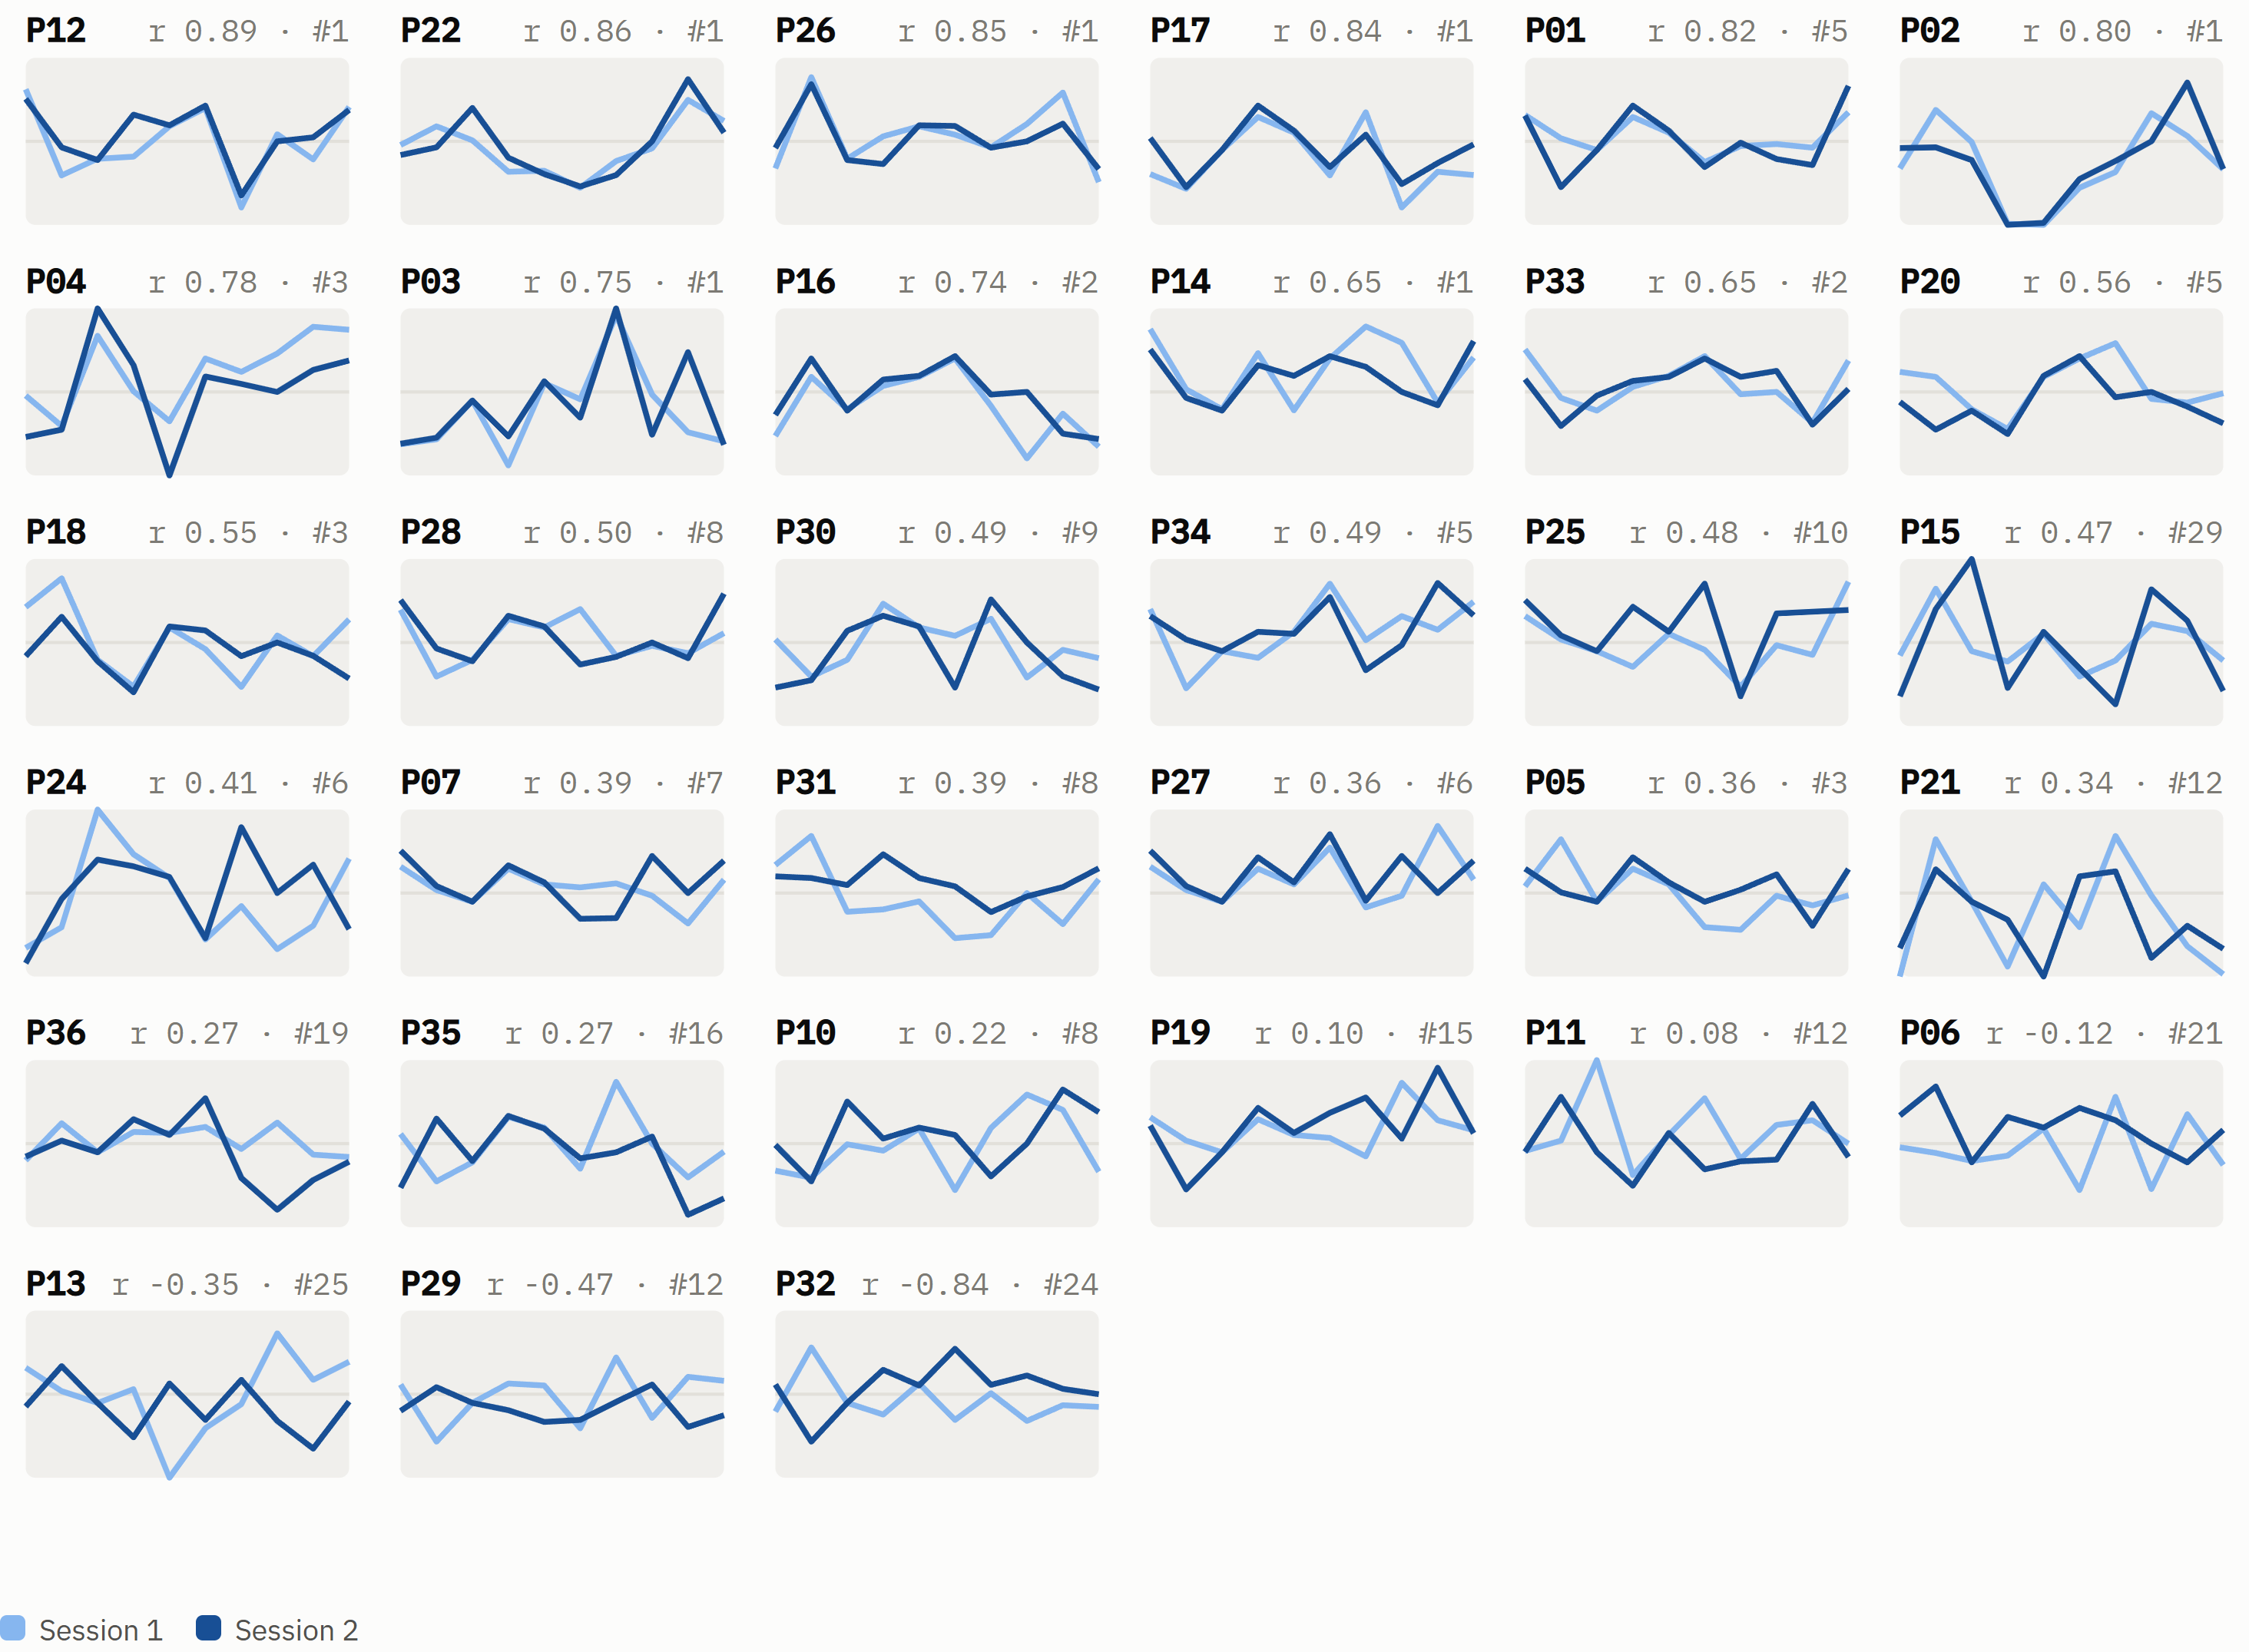
\includegraphics[width=\linewidth,height=0.55\textheight,keepaspectratio]{figs/results/f-personal-style__profiles__main.png}
\caption{\textbf{What a personal style looks like}}
\label{fig:res:personal-style:profiles}
\end{figure}

\paragraph*{Key numbers.}

\begin{itemize}[leftmargin=1.2em,itemsep=1pt]

\item 24 of 33 people have r $\geq$ .27 between their two sessions; 4 have r < 0

\end{itemize}

\paragraph*{Method.} {\small Each line joins the ten habit z-scores (within game, clipped at $\pm$2.5 for drawing). r = correlation of the two lines; \#k = where their own session 2 ranked among 33 (1 = nearest).}

\clearpage

\subsubsection{Which habits carry over --- and what each correlation means}\label{sec:res:personal-style:habit-by-habit}

\noindent \passtag{extra: may make it in}

\noindent \regtext{Each small scatter is one habit: a dot is a person, x = that habit in session 1, y = the same habit in session 2. If people kept their place in the queue exactly, the dots would lie on the dashed line; if session 1 told us nothing, they would be a shapeless cloud. Six of the ten habits carry over clearly: keeping Suggest plans, pressing Suggest, taking cards, previewing cards, decision time, and Suggest in recovery. Topping up drones on single-type missions does not carry over at all.} (Figure~\ref{fig:res:personal-style:habit-by-habit})

\begin{figure}[H]
\centering
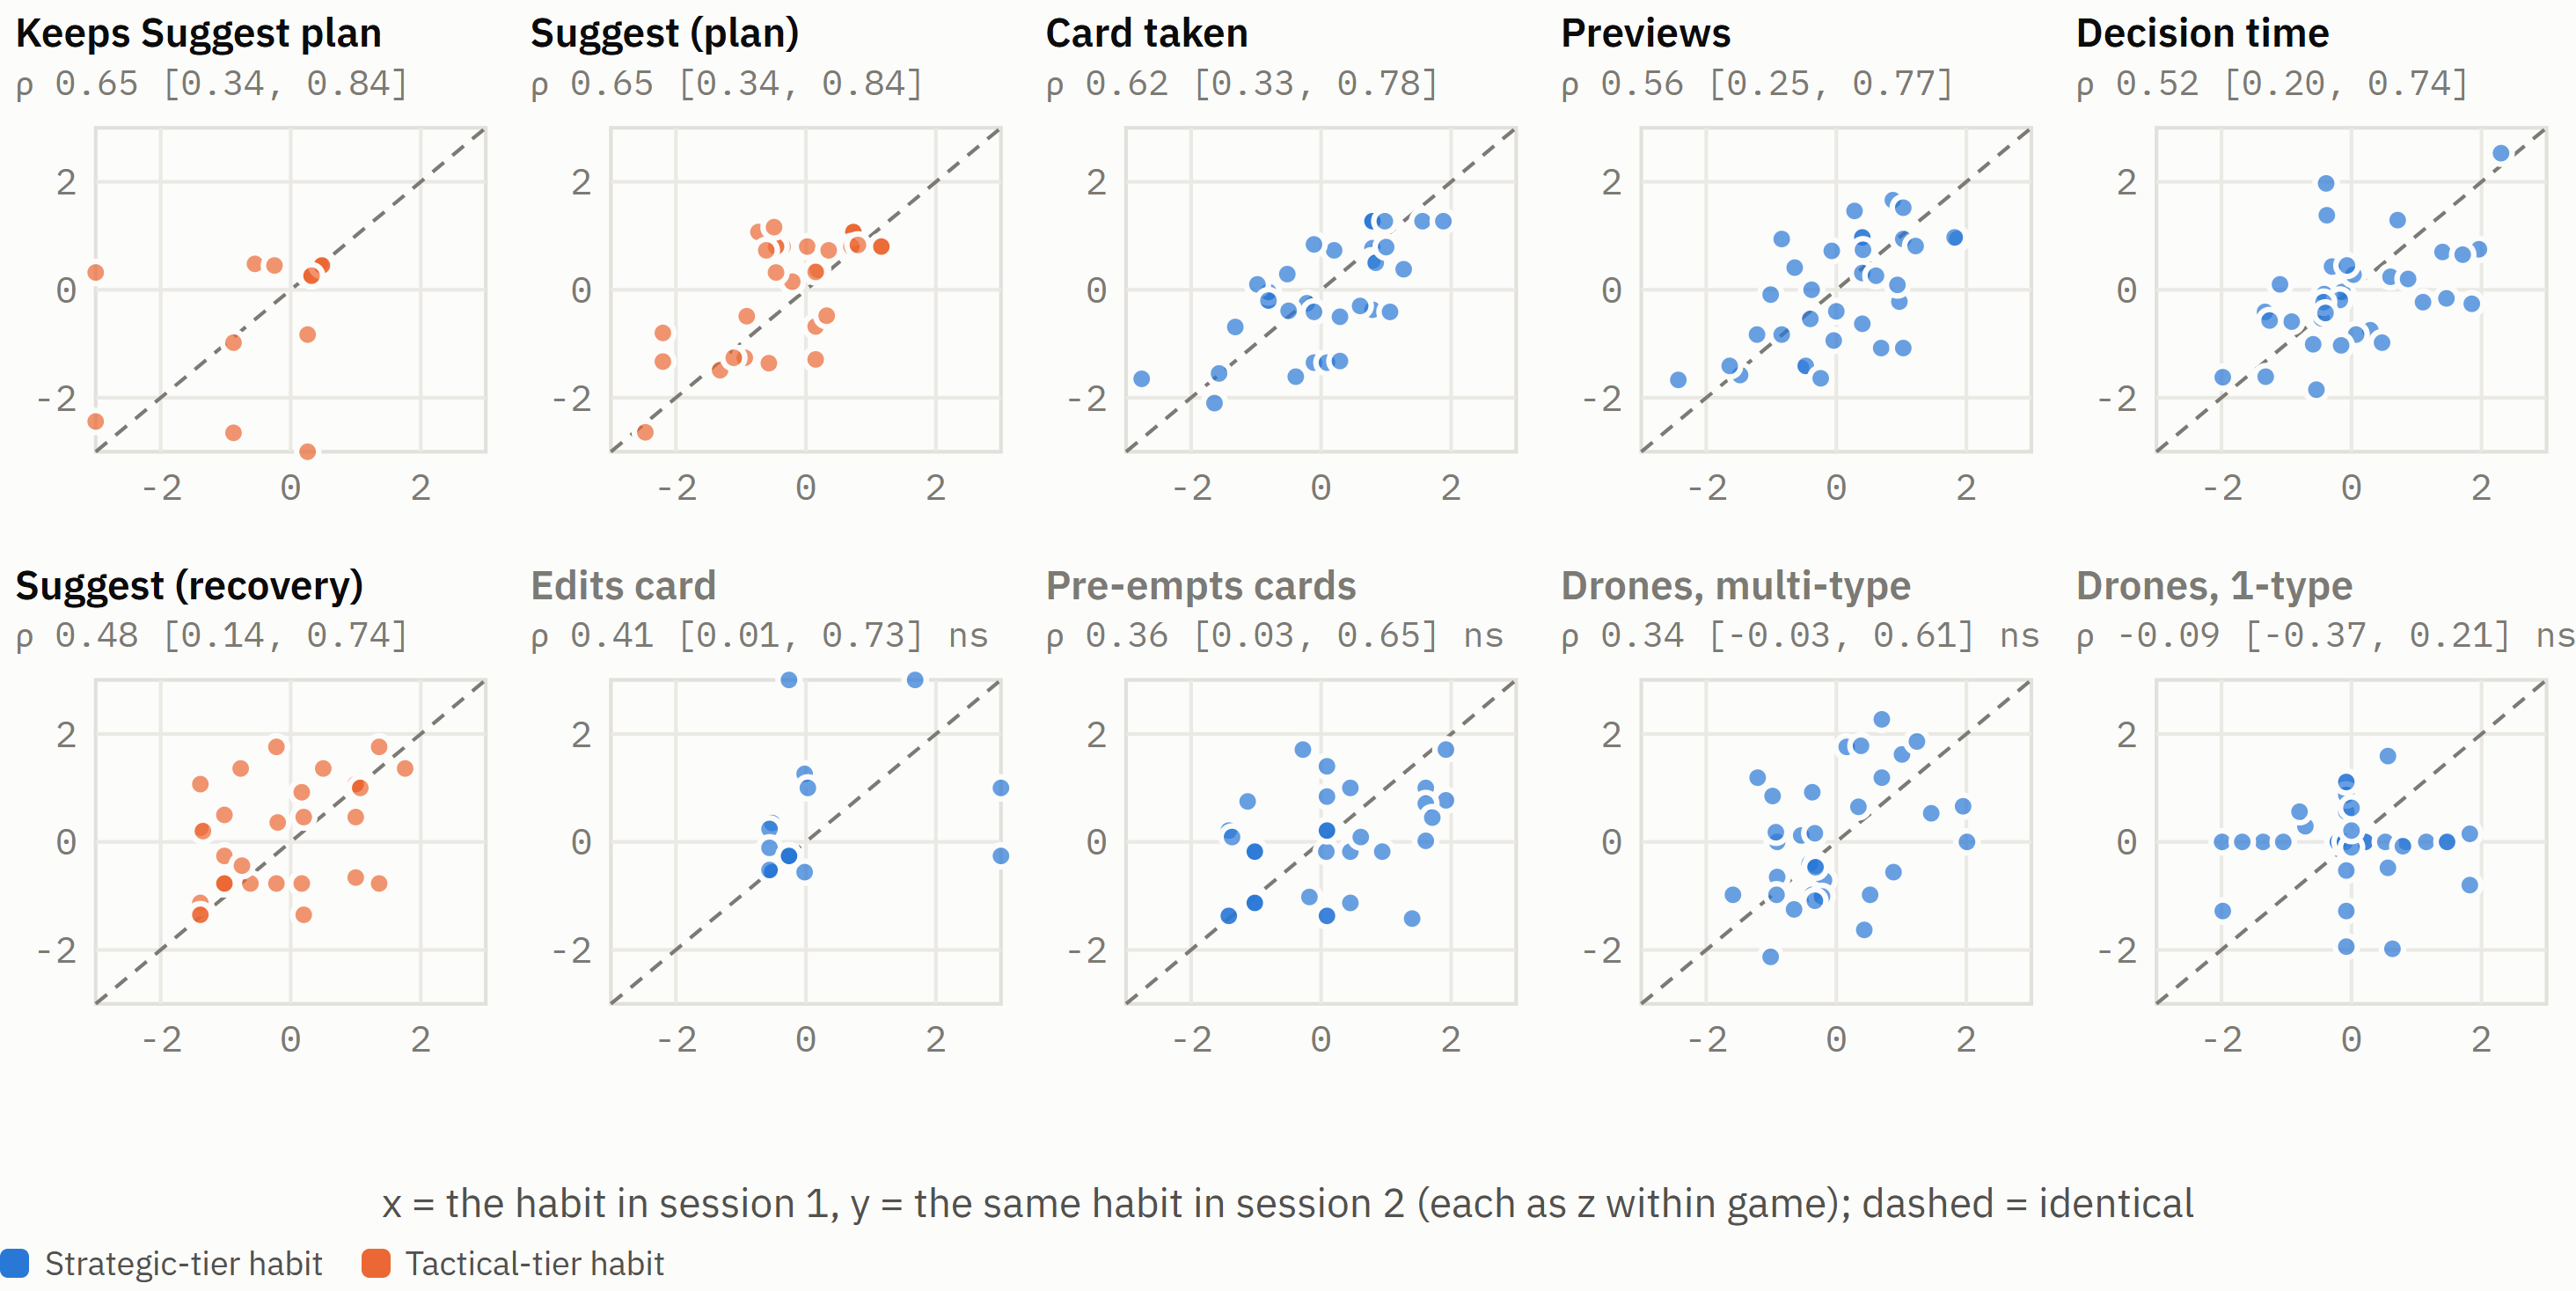
\includegraphics[width=\linewidth,height=0.55\textheight,keepaspectratio]{figs/results/f-personal-style__habit-by-habit__main.png}
\caption{\textbf{Which habits carry over --- and what each correlation means}}
\label{fig:res:personal-style:habit-by-habit}
\end{figure}

\paragraph*{Key numbers.}

\begin{itemize}[leftmargin=1.2em,itemsep=1pt]

\item Survive Holm: keeps Suggest plan $\rho$ .65 [.34, .84]; presses Suggest .65 [.34, .84]; takes card .62 [.33, .78]; previews .56 [.25, .77]; decision time .52 [.20, .74]; Suggest in recovery .48 [.14, .74]

\item Do not: edits a card .41; manual-before-cards (share of manual) .36; drones on multi-type .34; drones on single-type $-$.09

\item Card uptake: \textasciitilde{}2 distinct levels of people from one session, \textasciitilde{}3 from two

\item Score on the reliance axis, session 1 vs 2: $\rho$ = .65 [.38, .82]

\end{itemize}

\paragraph*{Method.} {\small $\rho$ (Spearman) for habit X = the correlation, across the 33 people, between their rank on X in session 1 and their rank on X in session 2, each session first adjusted for the game played (z within game). $\rho$ = .62 for ``takes the strategy card'' means people keep roughly the same order: high card-takers in session 1 are mostly high in session 2, though not exactly. 95\% intervals come from resampling people 2000 times; Holm corrects for testing ten habits. ``Distinct levels'' (separation strata) says how many groups of people the habit can tell apart reliably: one session of card uptake separates about 2 (high vs low), the average of two sessions about 3. Caution on ``keeps the Suggest plan'': 24 of 33 people kept every Suggest plan unchanged in both sessions (a ceiling), so its high $\rho$ mostly says that the nine who ever edit a plan tend to do so in both sessions. The pre-empting habit here is ``share of \emph{manual} choices made before the cards loaded'' (undefined for 15 people who never chose manual in a session); the clearer per-decision version is in the next section.}

\clearpage

\subsubsection{Not waiting for the cards is one of those habits}\label{sec:res:personal-style:preempt}

\noindent \passtag{extra: may make it in}

\noindent \regtext{Committing a manual allocation before the strategy cards have even loaded is something some people do and others never do. People who did it in session 1 did it on a quarter of their decisions in session 2; people who did not, on 8\%. Fifteen people never did it in either session.} (Figure~\ref{fig:res:personal-style:preempt})

\begin{figure}[H]
\centering
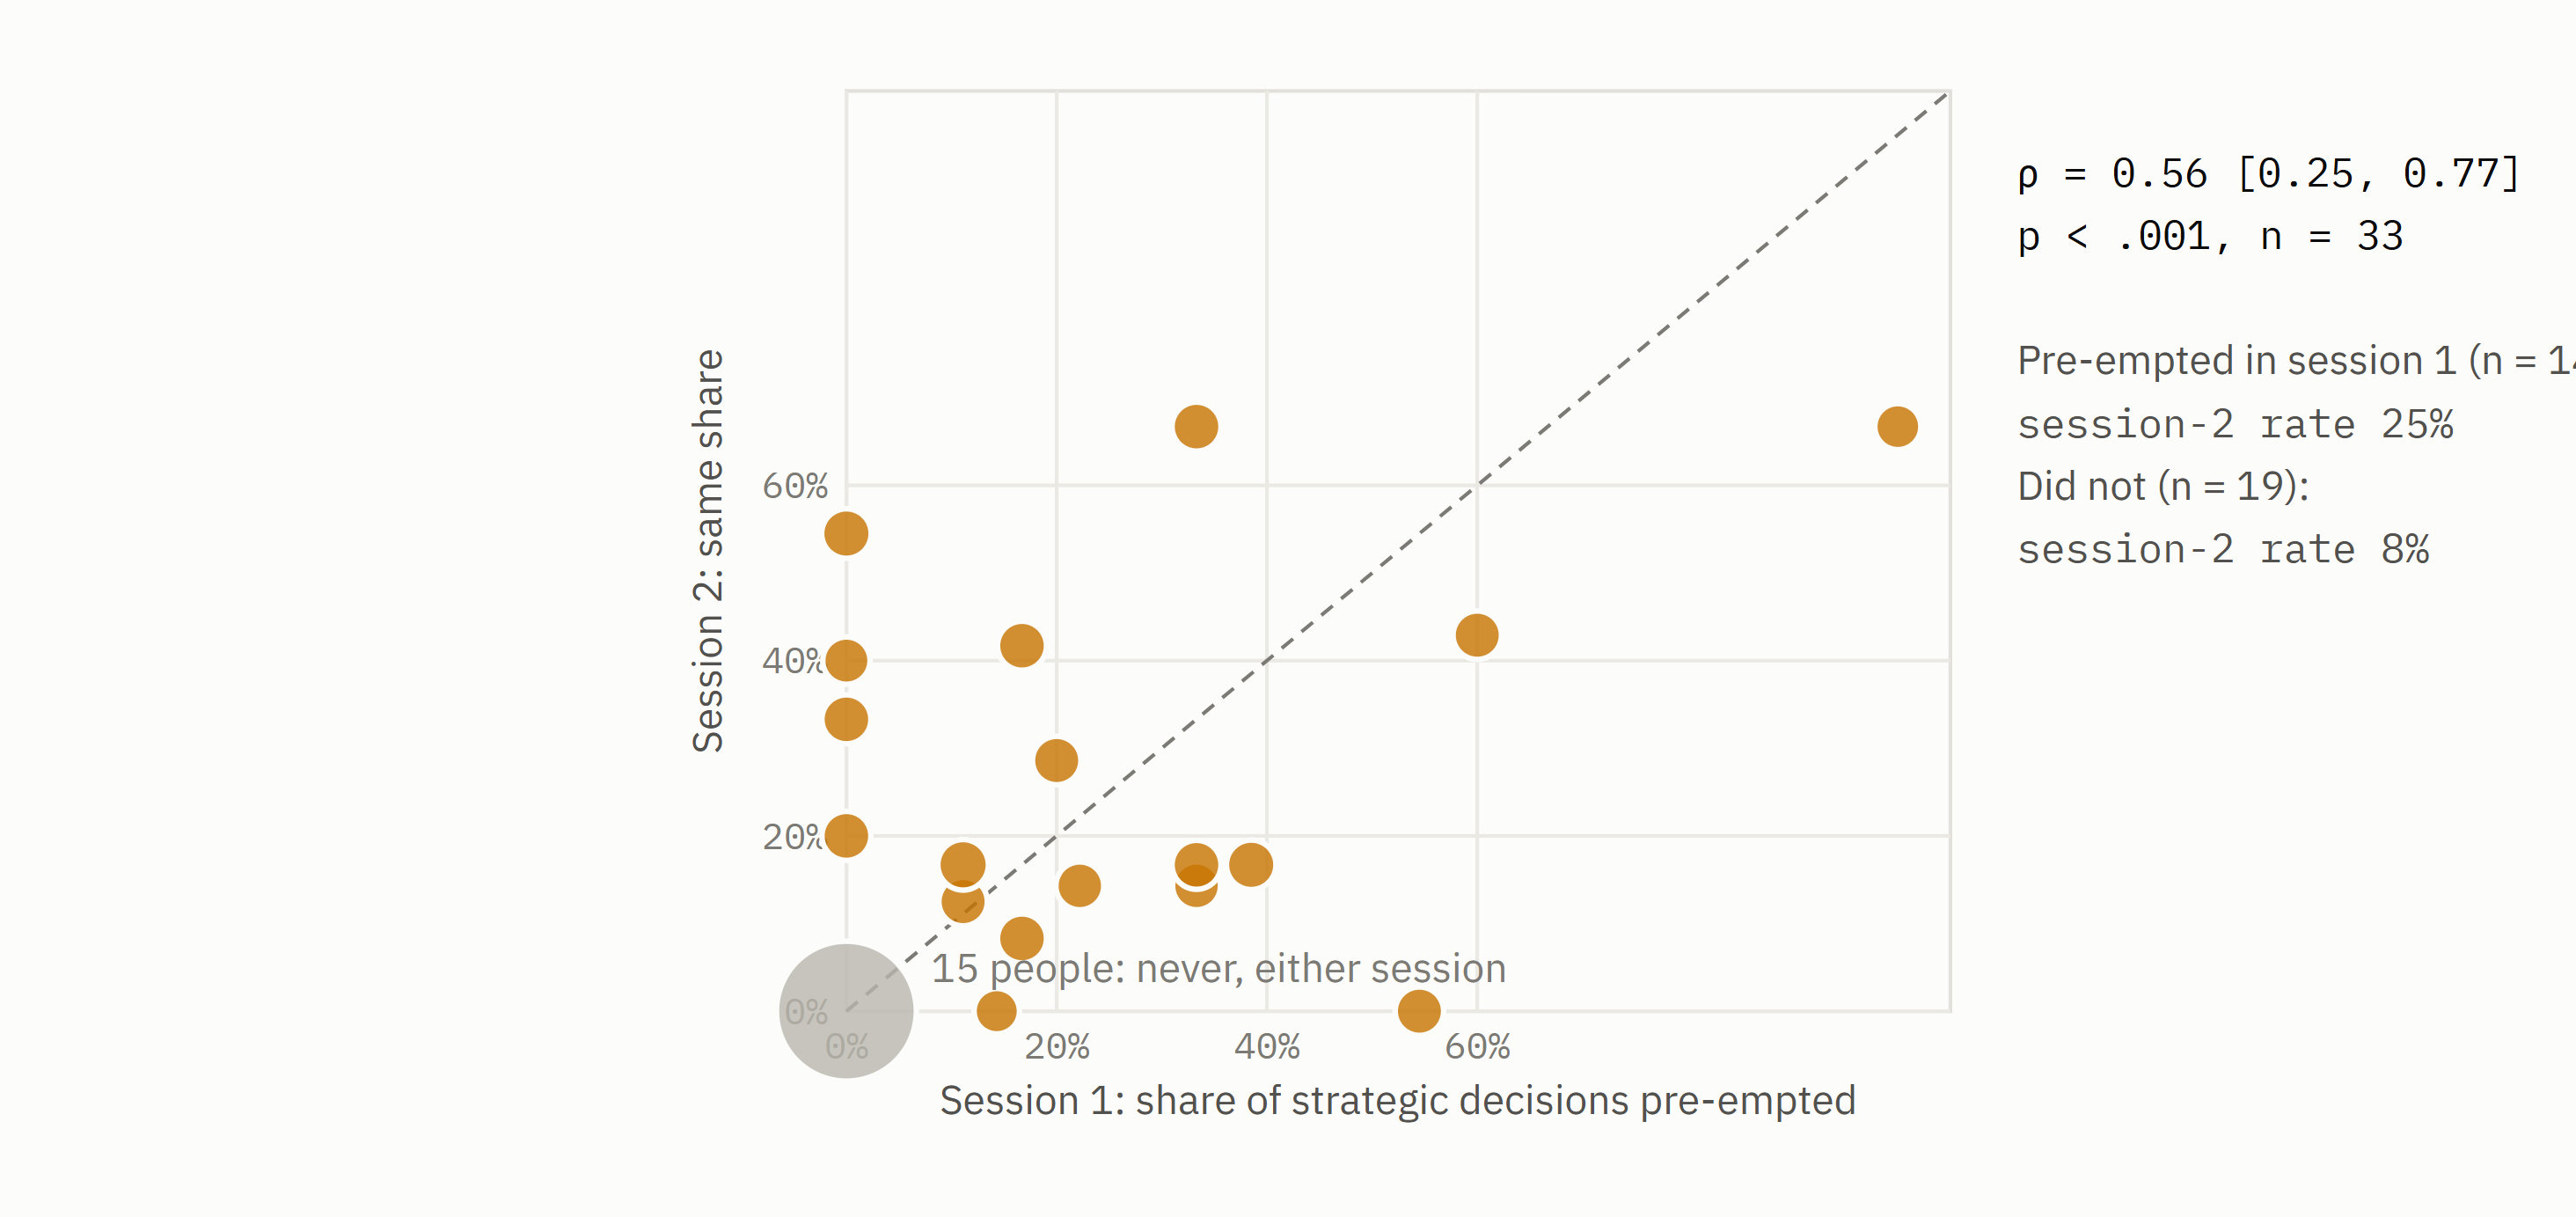
\includegraphics[width=\linewidth,height=0.55\textheight,keepaspectratio]{figs/results/f-personal-style__preempt__main.png}
\caption{\textbf{Not waiting for the cards is one of those habits}}
\label{fig:res:personal-style:preempt}
\end{figure}

\paragraph*{Key numbers.}

\begin{itemize}[leftmargin=1.2em,itemsep=1pt]

\item Session 1 vs 2: $\rho$ = .56 [.25, .77], p < .001, n = 33

\item Session-2 rate 25\% for those who pre-empted in session 1 (n = 14) vs 8\% for those who did not (n = 19)

\item 86 of 564 decisions pre-empted; 46\% of all manual choices; 15 of 33 never did it

\item Round 2: person share of variance .24, mission .05

\end{itemize}

\paragraph*{Method.} {\small Rows: 564 non-residual strategic decisions. Per person and session: share of decisions committed manually before the cards appeared (logged \texttt{manualBeforeCardsLoaded}). $\rho$ = Spearman of the session-1 share against the session-2 share across 33 people. Variance shares (person \textasciitilde{}24\%, mission \textasciitilde{}5\%) are from round 2 (F4.1, crossed random intercepts for person and the exact mission, which repeats across people because games are fixed). The 15 ``never'' people sit together at the origin; $\rho$ is driven both by them staying at zero and by the regular pre-empters staying high.}

\clearpage

\subsection{Small jobs by hand, big jobs to the assistant --- on both tiers, and it is where the assistant saves time (supplementary analyses)}\label{sec:sup:res:size-decides}

\noindent Supplement to Section~\ref{sec:res:size-decides}.

\subsubsection{Is it an artefact? Checks, all reported}\label{sec:res:size-decides:artefacts}

\noindent \passtag{numbers only}

\noindent \regtext{The worry: the illogical Conservative card (one that adds a drone of a type the mission does not need) appears only on one- and two-type missions --- 71\% of one-type decisions, none of the three-type ones --- so ``people avoid the card on small missions'' could be ``people avoid a visibly odd card''. It is not: on one-type missions uptake is the same with an odd card (50\%, 129 decisions) and without one (56\%, 52 decisions), and with every odd-card decision removed the size effect is still there ($\times$1.46 per doubling; clean one-type vs three-type $\times$1.83). No $\varepsilon$-corrupted (deliberately wrong) cards were shown in any session, so card quality did not otherwise vary by size. The rule also holds with queue length held fixed, with the minute of session held fixed, per session, per scenario, without the half-weight participants and in a person-fixed-effects model. Two strategic rows do not reach p < .05: Tactical Heavy sessions alone (few one-type missions there) and cards-on-screen only (above). The tactical rule clears every row.} (Figure~\ref{fig:res:size-decides:artefacts})

\begin{figure}[H]
\centering
\begin{subfigure}[t]{\linewidth}
\centering
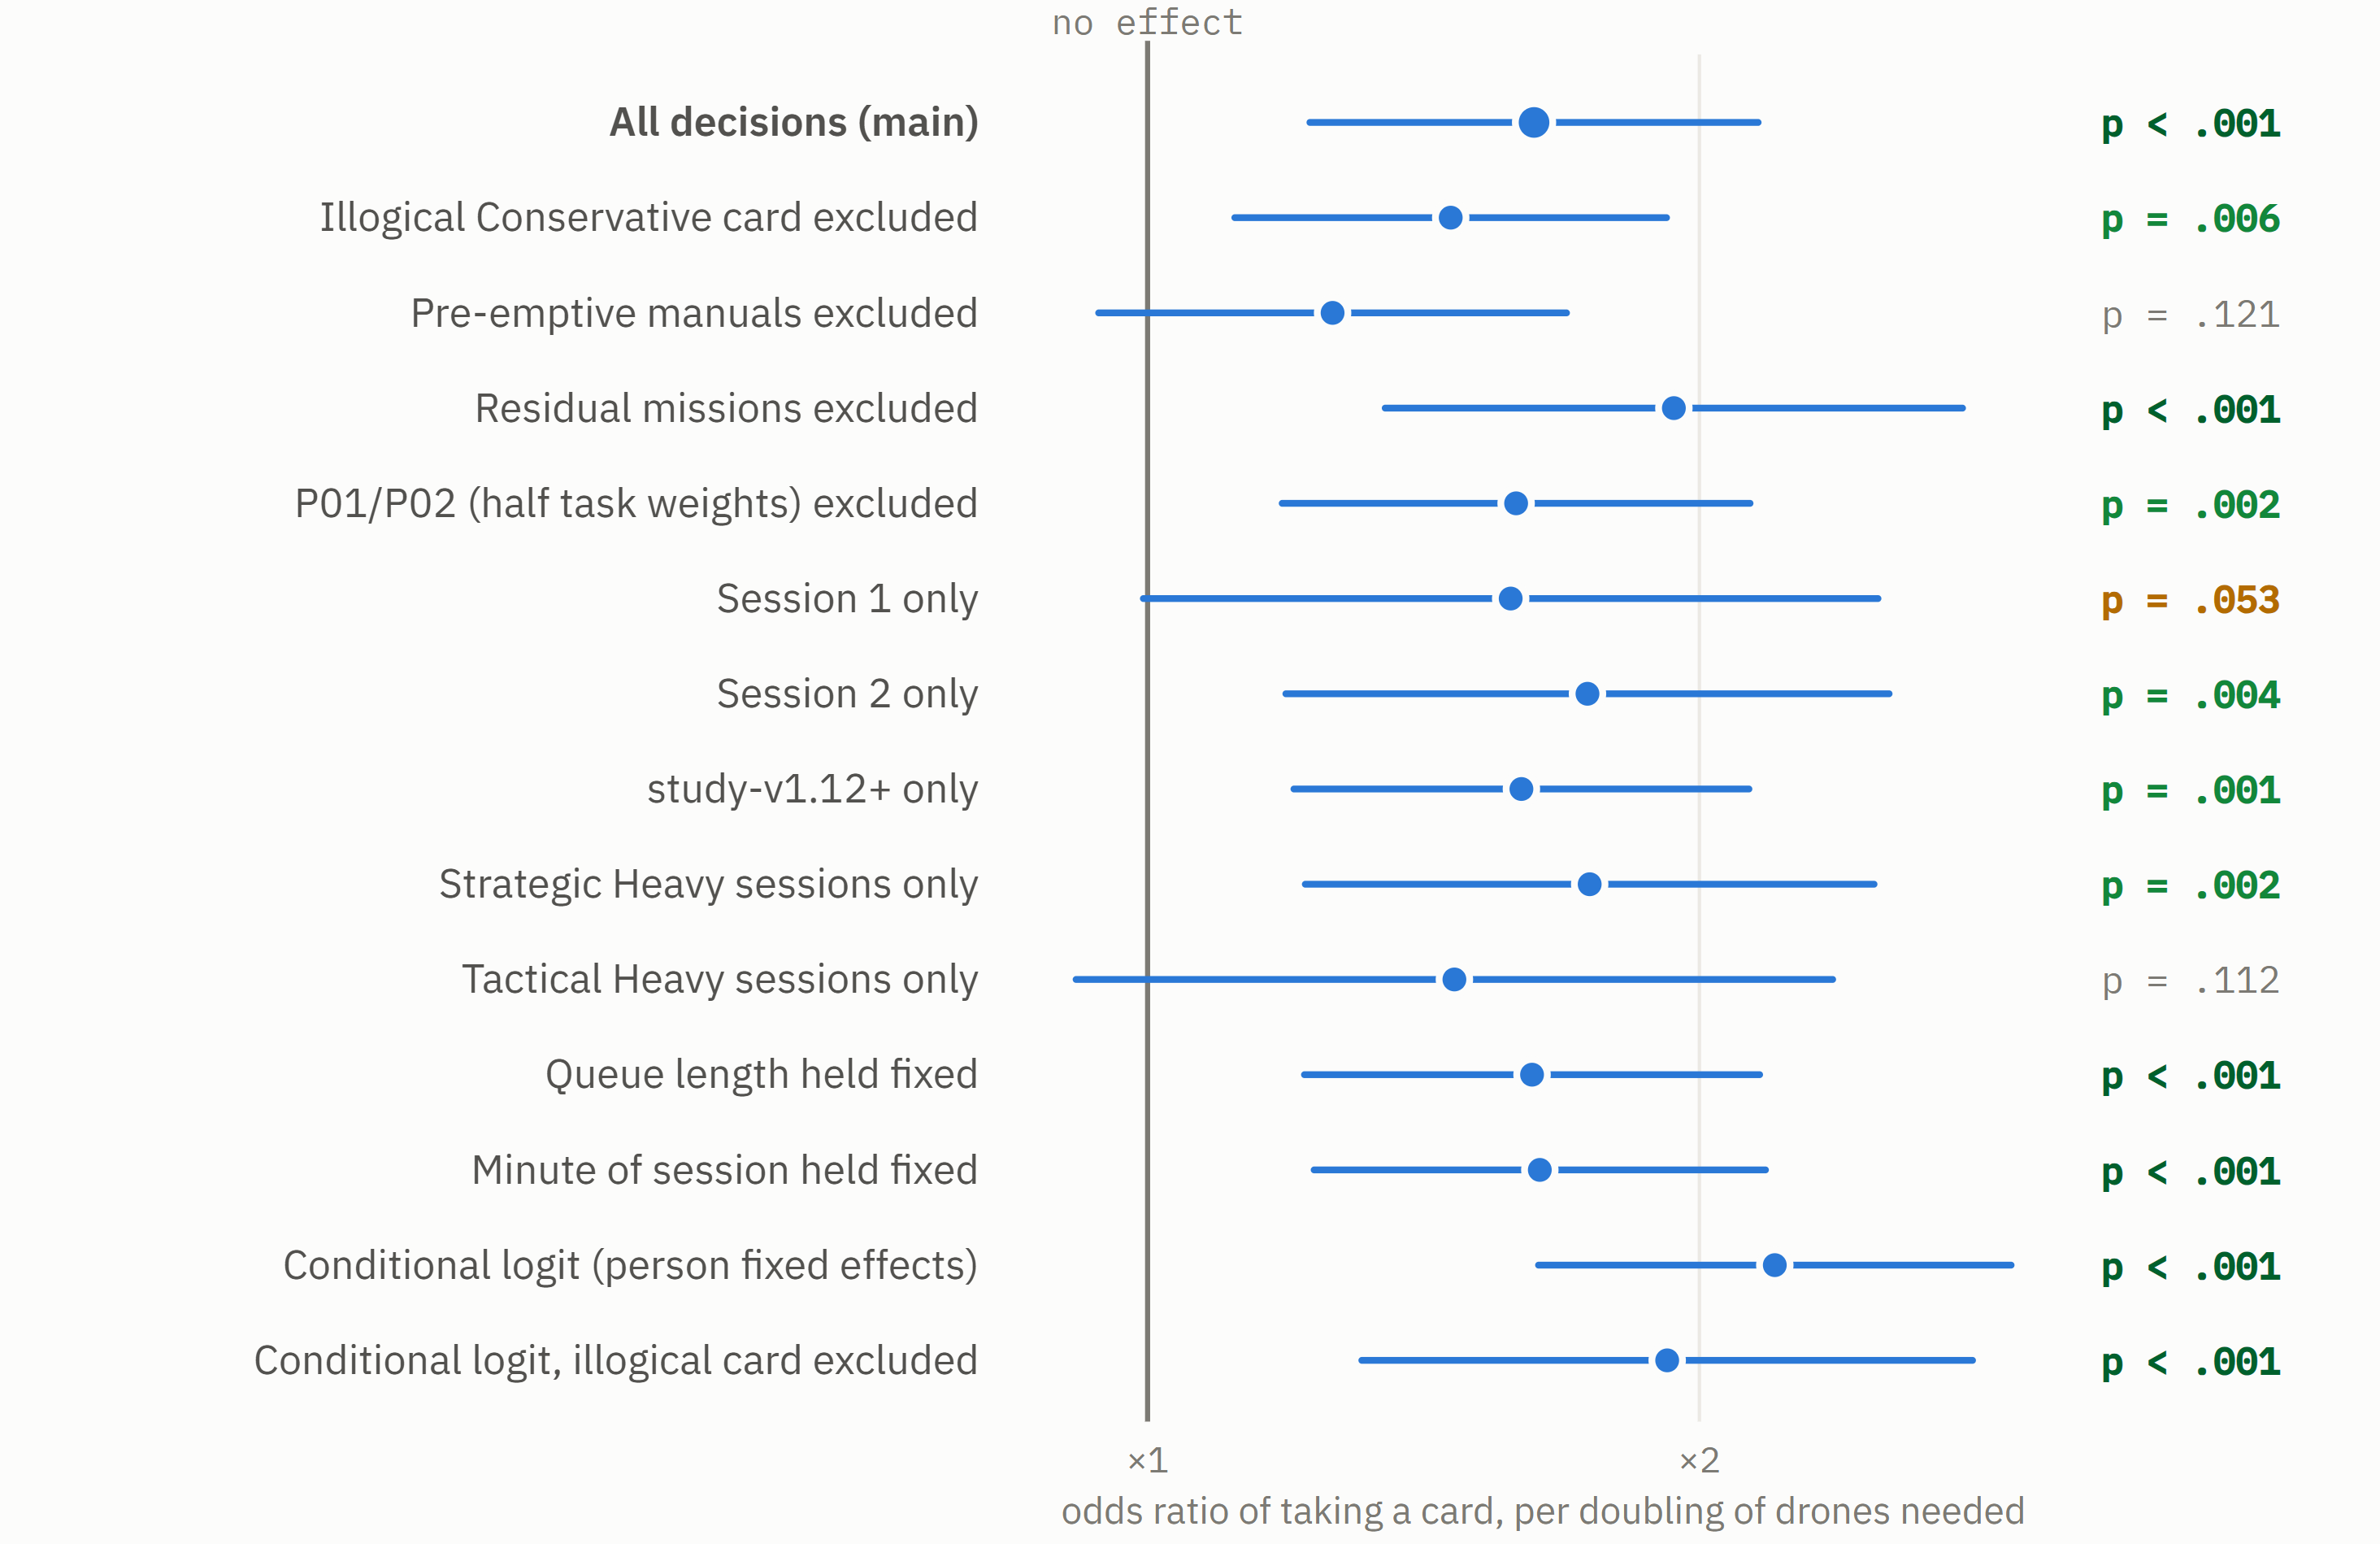
\includegraphics[width=\linewidth,height=0.23\textheight,keepaspectratio]{figs/results/f-size-decides__artefacts__strat.png}
\caption{Strategic tier.}
\label{fig:res:size-decides:artefacts:strat}
\end{subfigure}
\par\smallskip
\begin{subfigure}[t]{\linewidth}
\centering
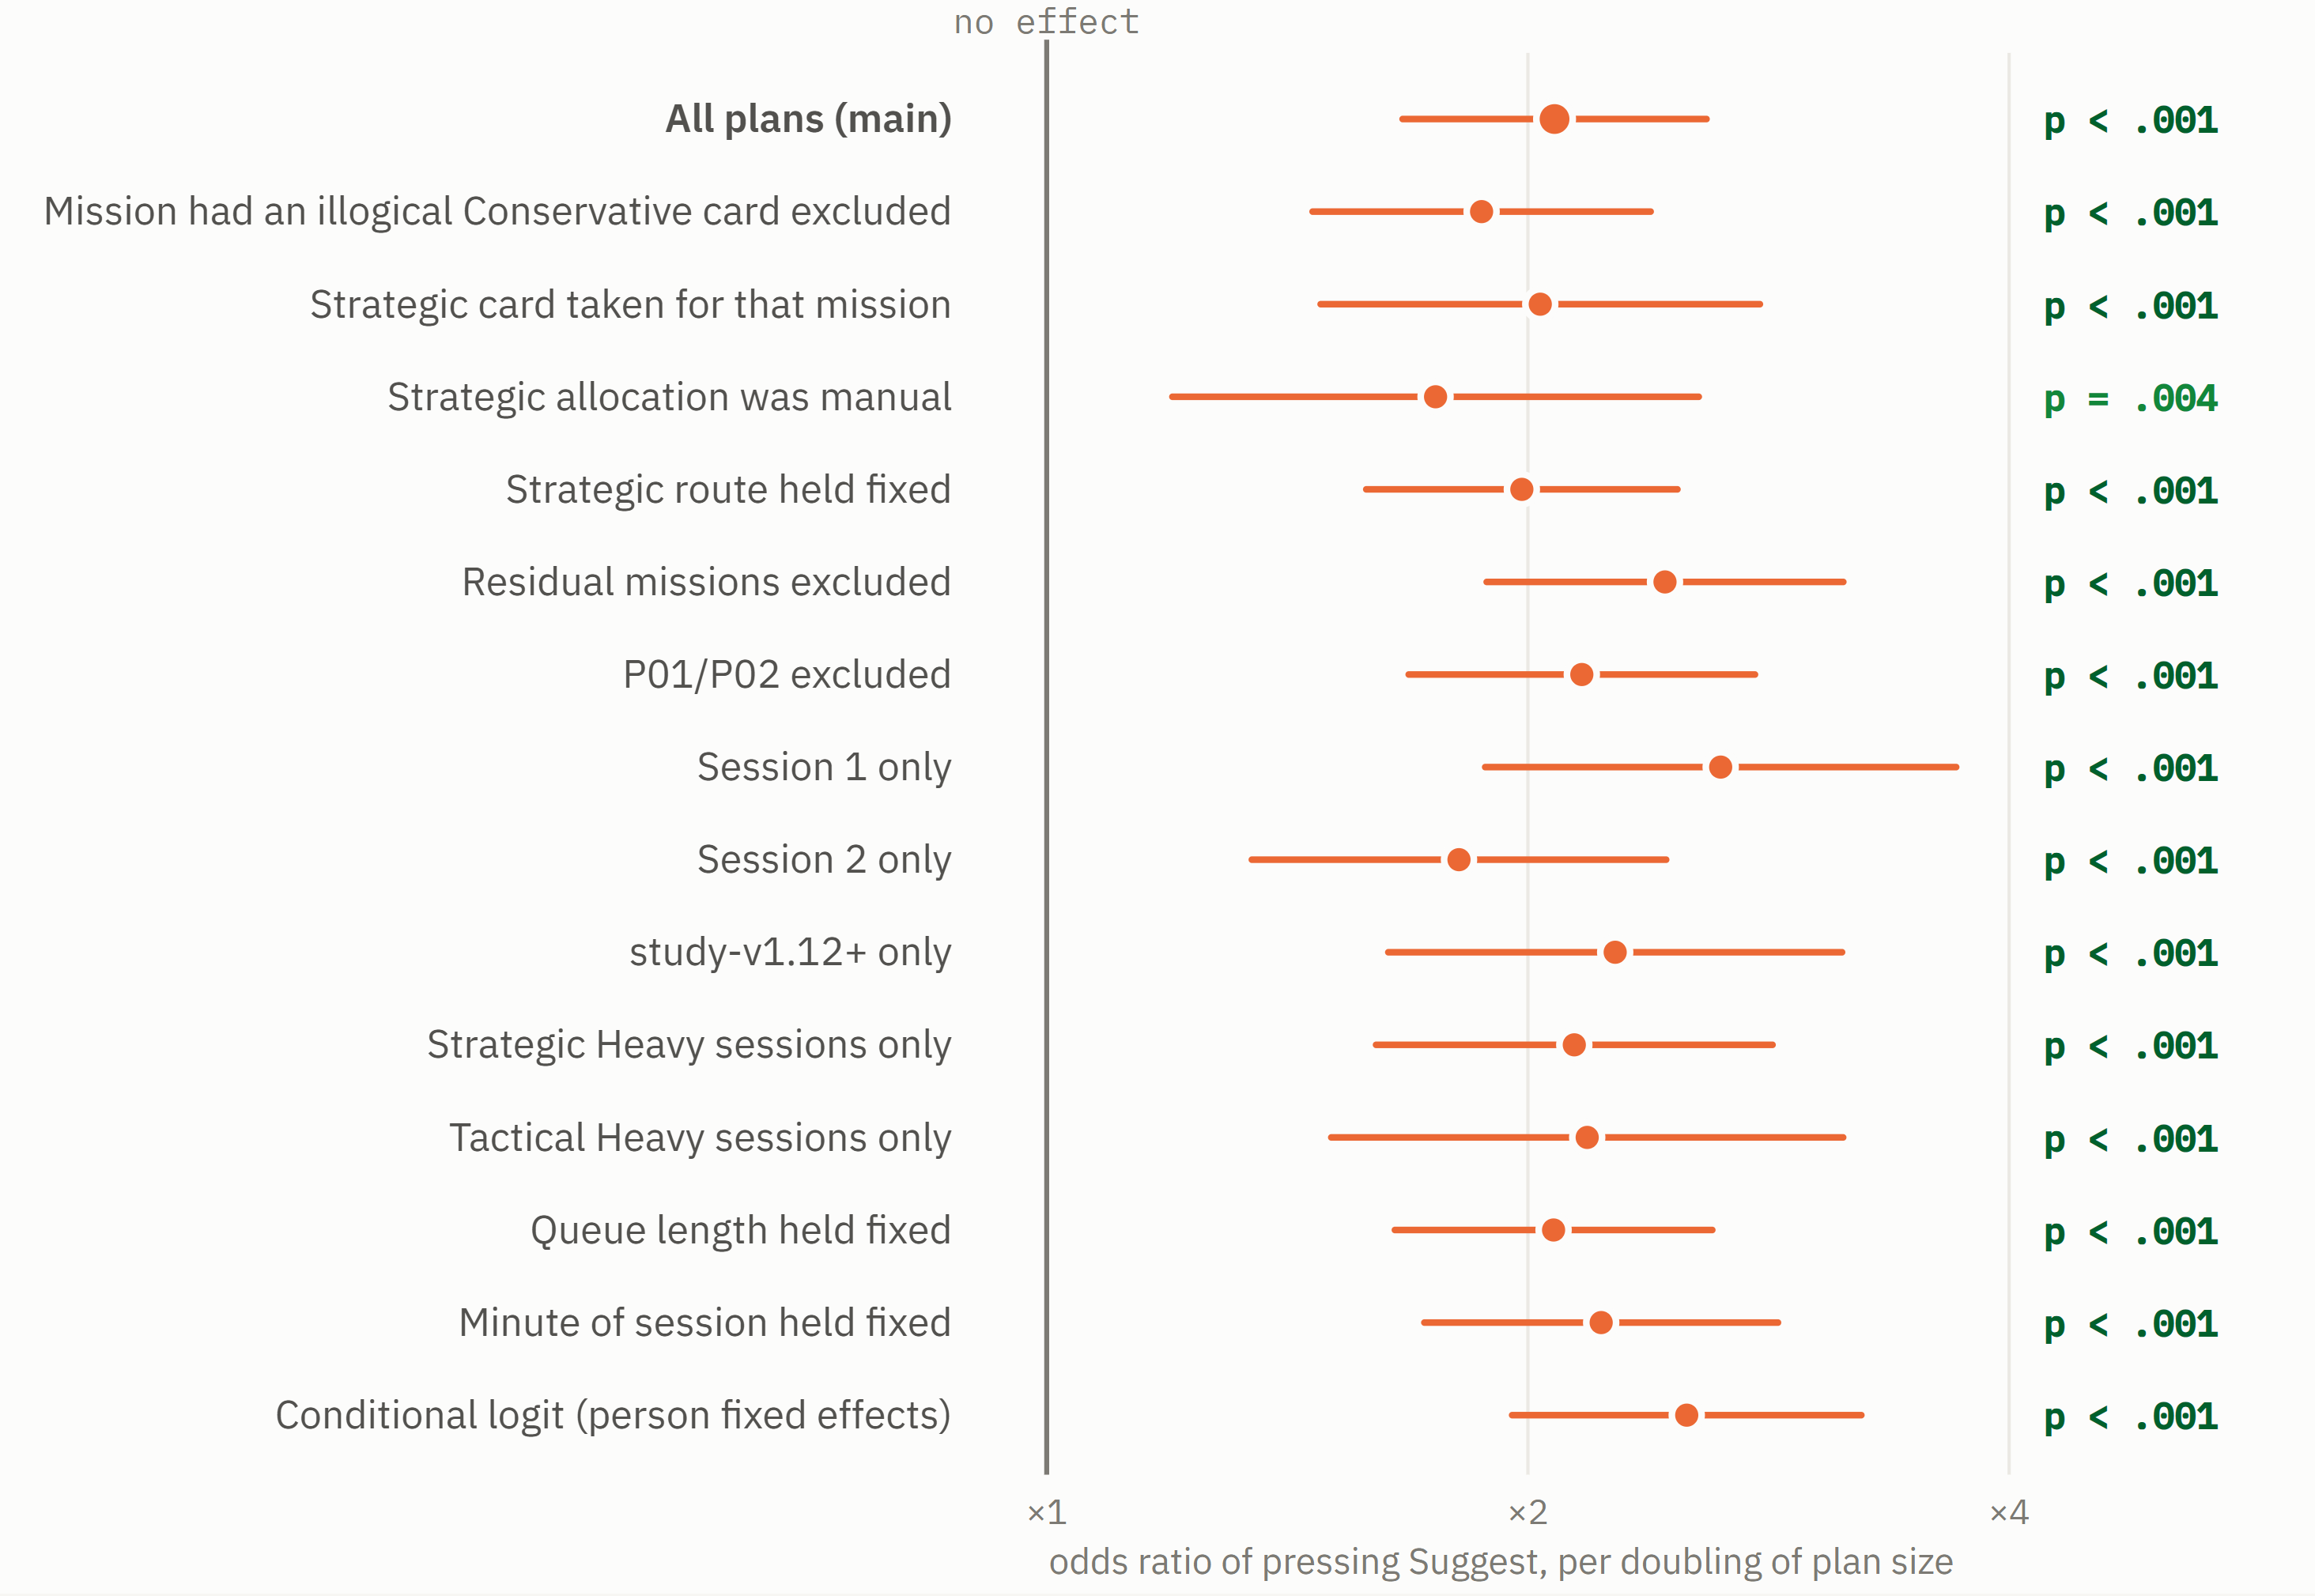
\includegraphics[width=\linewidth,height=0.23\textheight,keepaspectratio]{figs/results/f-size-decides__artefacts__tac.png}
\caption{Tactical tier.}
\label{fig:res:size-decides:artefacts:tac}
\end{subfigure}
\par\smallskip
\caption{\textbf{Is it an artefact? Checks, all reported}}
\label{fig:res:size-decides:artefacts}
\end{figure}

\paragraph*{Key numbers.}

\begin{itemize}[leftmargin=1.2em,itemsep=1pt]

\item Strategic, illogical card excluded: $\times$1.46 [1.12, 1.92], p = .006 (474 decisions); conditional logit $\times$1.92 [1.31, 2.82]

\item One-type missions, odd card vs clean card: odds $\times$0.77 [0.33, 1.78], p = .55 --- no difference

\item Strategic range across 14 specifications: $\times$1.26 to $\times$2.20; tactical range across 15: $\times$1.75 to $\times$2.64

\item Tactical, illogical-card missions excluded: $\times$1.87 [1.47, 2.39]; strategic route held fixed $\times$1.98

\end{itemize}

\paragraph*{Method.} {\small Each row refits the main within-person model on a subset or with one more control. Illogical card: the \emph{odd} flag from build\_findings\_synthesis.load\_decisions (Conservative card carries a type the mission needs none of). Queue held fixed: the number of missions waiting at the decision, split within/between person (the queue story itself is Section~\ref{sec:res:workload}'s). Conditional logit: a different model family that compares each person only with themselves by construction (people who always or never hand over drop out, hence fewer people). The odd-card story itself is Section~\ref{sec:res:flaw-odd}'s --- here it is only checked as a confound.}

\clearpage

\subsubsection{Person by person}\label{sec:res:size-decides:people}

\noindent \passtag{extra: may make it in}

\noindent \regtext{The same rule with each person counted once: for each band of mission size, each person's own hand-over rate, averaged over people. The default view removes each person's overall level first, so it shows how the \emph{same} people shift between small and big missions. Both tiers rise band by band. 22 of 33 people hand over more on their biggest band than their smallest, on each tier; only 4 (strategic) and 2 (tactical) do the reverse.} (Figure~\ref{fig:res:size-decides:people})

\begin{figure}[H]
\centering
\begin{subfigure}[t]{\linewidth}
\centering
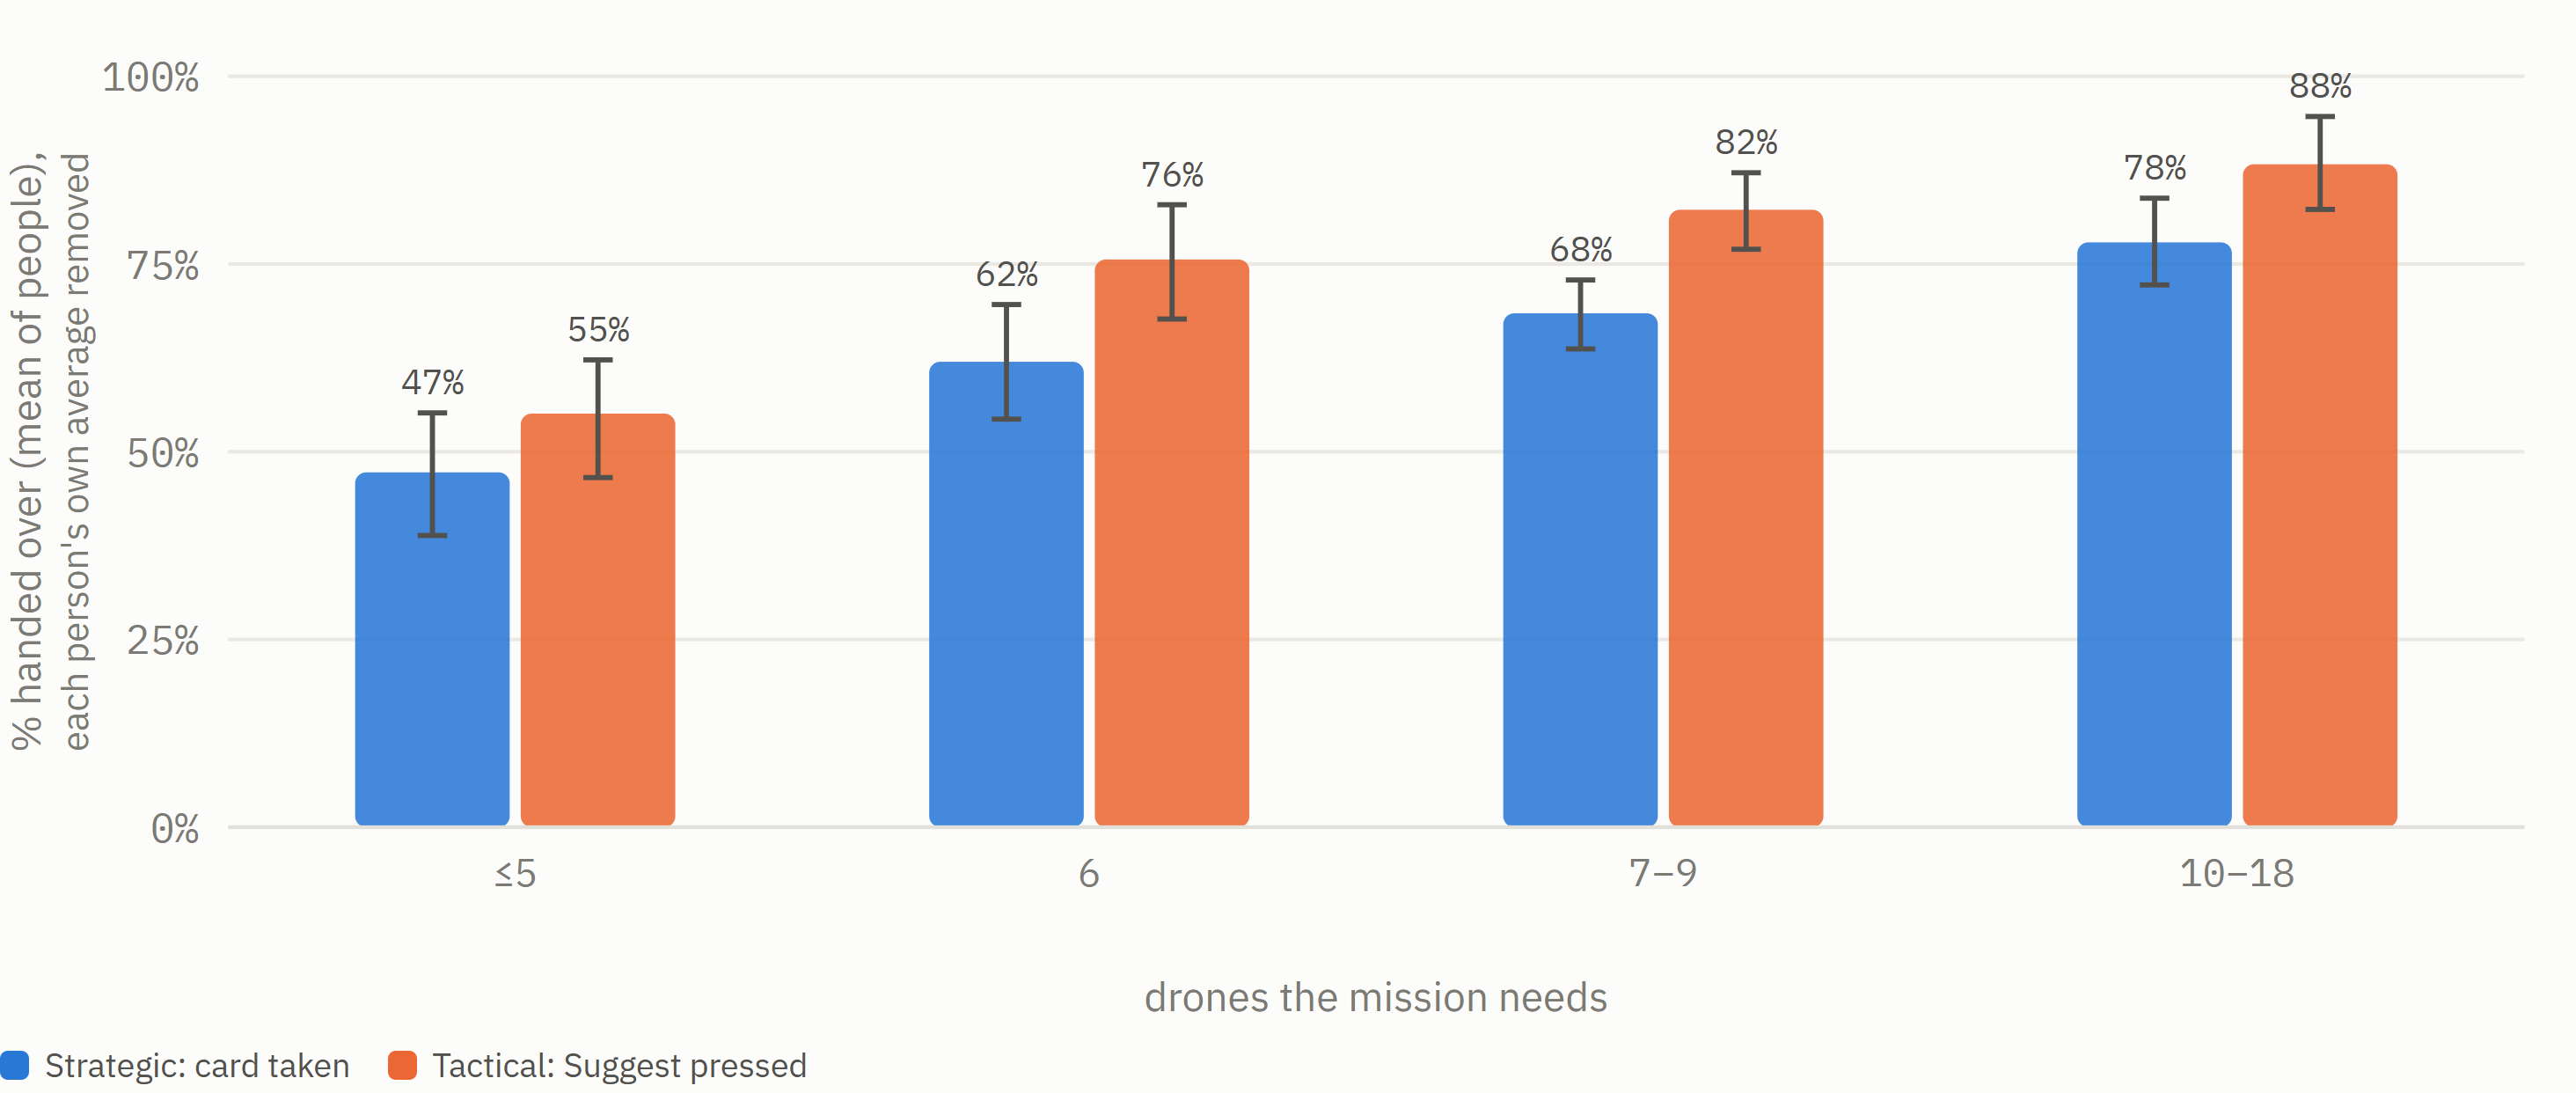
\includegraphics[width=\linewidth,height=0.23\textheight,keepaspectratio]{figs/results/f-size-decides__people__own.png}
\caption{Each person compared with their own average.}
\label{fig:res:size-decides:people:own}
\end{subfigure}
\par\smallskip
\begin{subfigure}[t]{\linewidth}
\centering
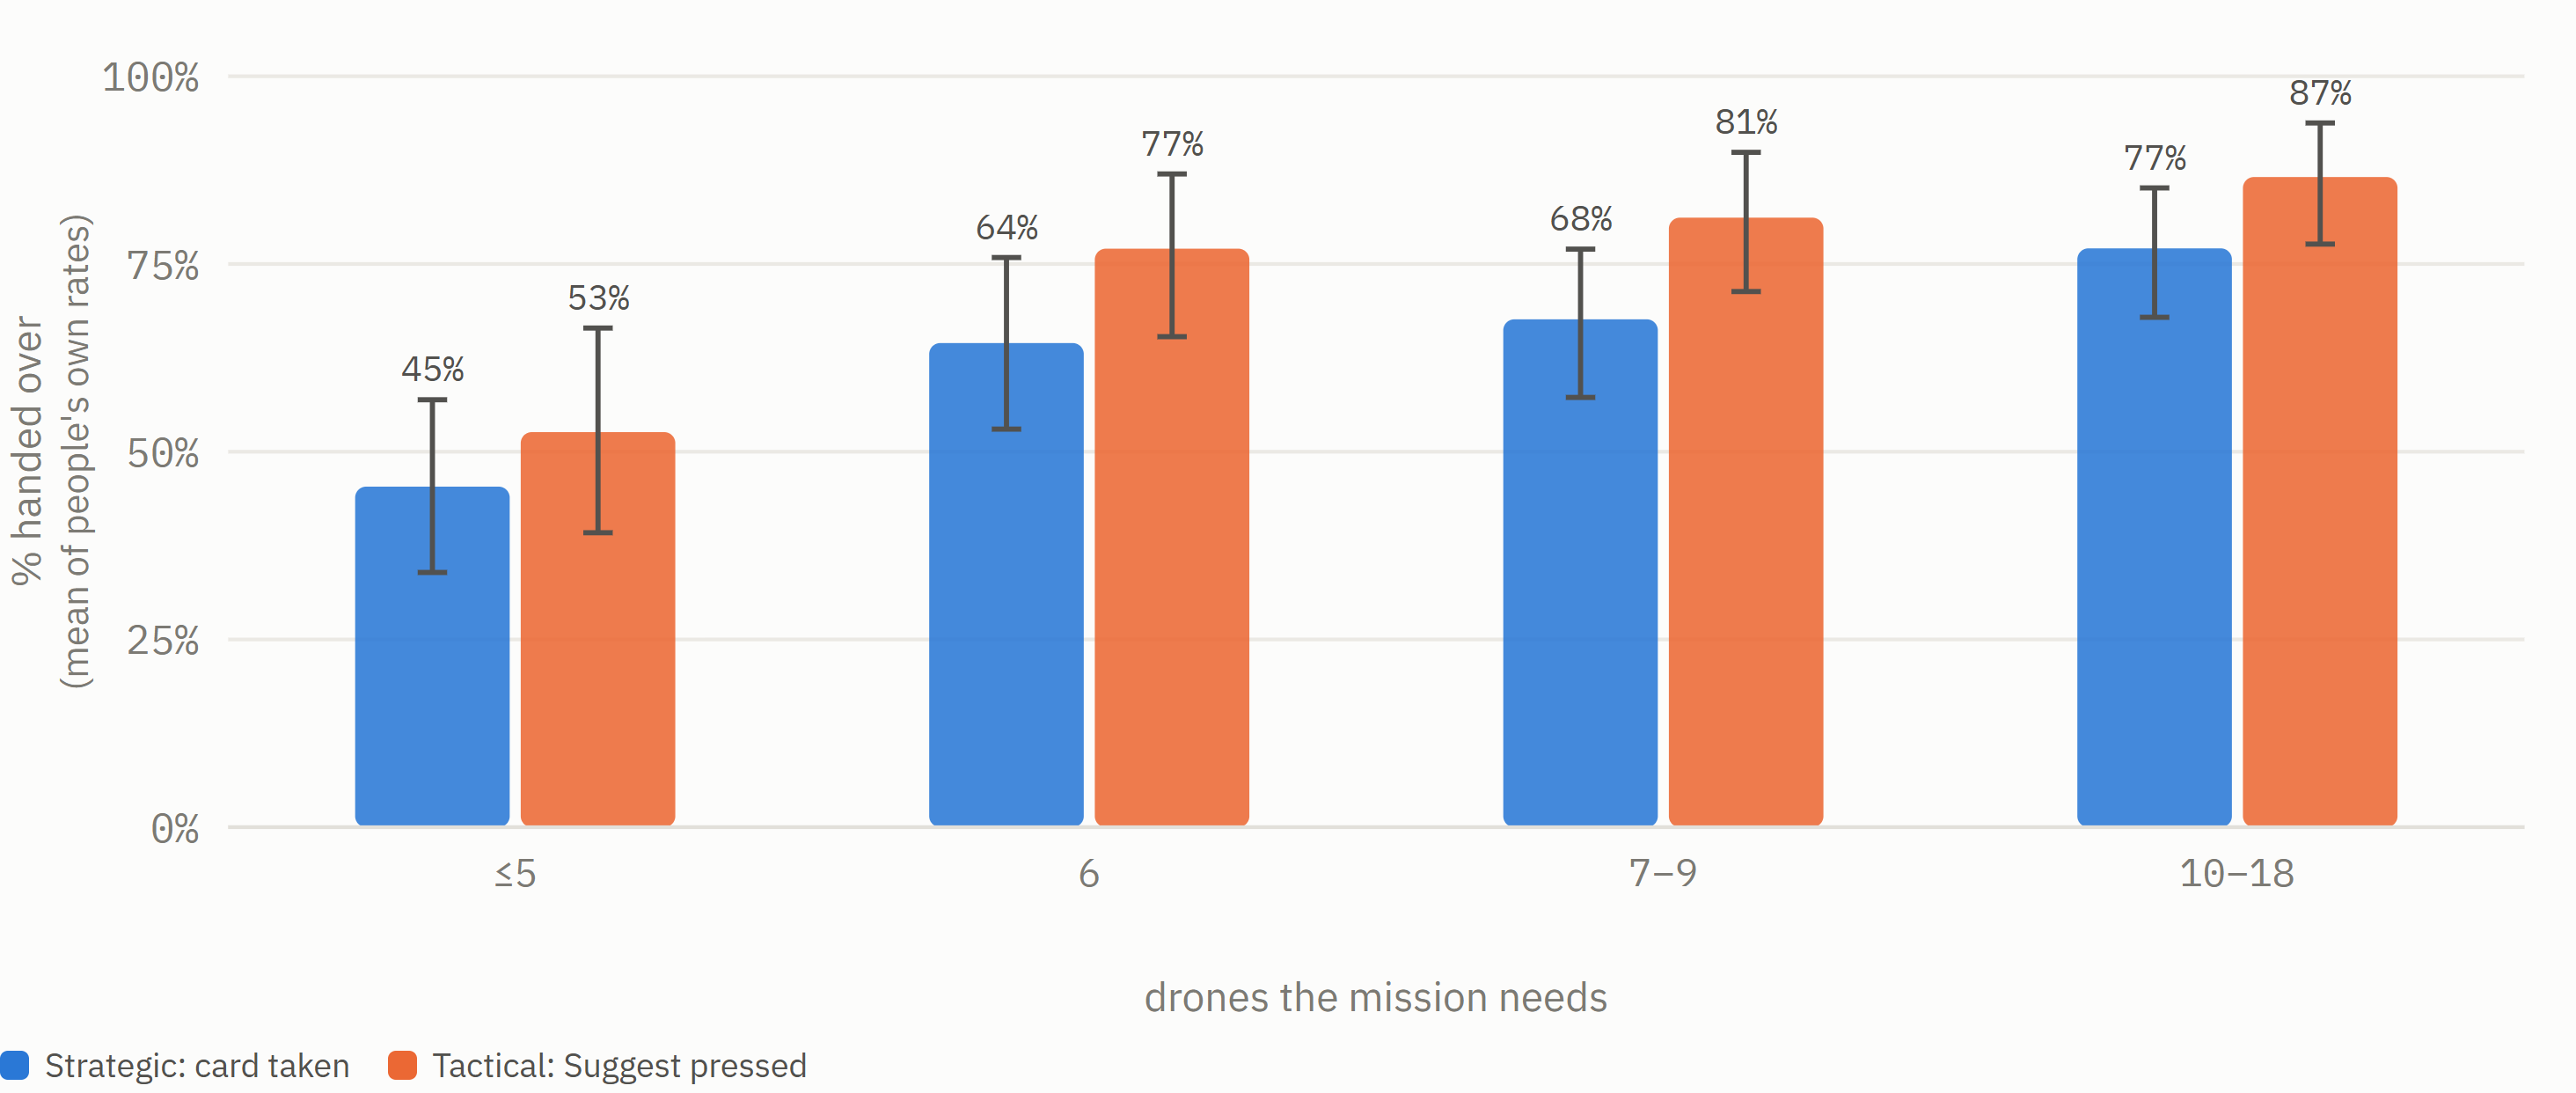
\includegraphics[width=\linewidth,height=0.23\textheight,keepaspectratio]{figs/results/f-size-decides__people__plain.png}
\caption{Plain average of people.}
\label{fig:res:size-decides:people:plain}
\end{subfigure}
\par\smallskip
\caption{\textbf{Person by person}}
\label{fig:res:size-decides:people}
\end{figure}

\paragraph*{Key numbers.}

\begin{itemize}[leftmargin=1.2em,itemsep=1pt]

\item Strategic, own average removed: 47\% ($\leq$5 drones, 32 people) $\rightarrow$ 62\% $\rightarrow$ 68\% $\rightarrow$ 78\% (10--18, 33 people)

\item Tactical, own average removed: 55\% $\rightarrow$ 76\% $\rightarrow$ 82\% $\rightarrow$ 88\%

\item Biggest band above smallest: strategic 22 people, below 4, equal 7 (sign test p < .001); tactical 22, 2, 9 (p < .001)

\end{itemize}

\paragraph*{Method.} {\small Bands of drones needed: $\leq$5, 6, 7--9, 10--18 (both tiers; drones needed is the measure both tiers share). A person contributes to a band if they made at least 2 decisions in it. ``Own average removed'' = the person's rate in the band minus their rate over all bands, plus the overall rate, so bars stay on the percentage scale. Whiskers: 95\% intervals from resampling people. Sign test: for each person, their biggest band against their smallest; are ``more'' more common than ``less'' than a coin flip would give (ties dropped)?}

\clearpage

\subsubsection{The speed difference as estimates}\label{sec:res:size-decides:speed-model}

\noindent \passtag{numbers only}

\noindent \regtext{The same comparison as model estimates: negative means the assistant route was faster for the same person.} (Figure~\ref{fig:res:size-decides:speed-model})

\begin{figure}[H]
\centering
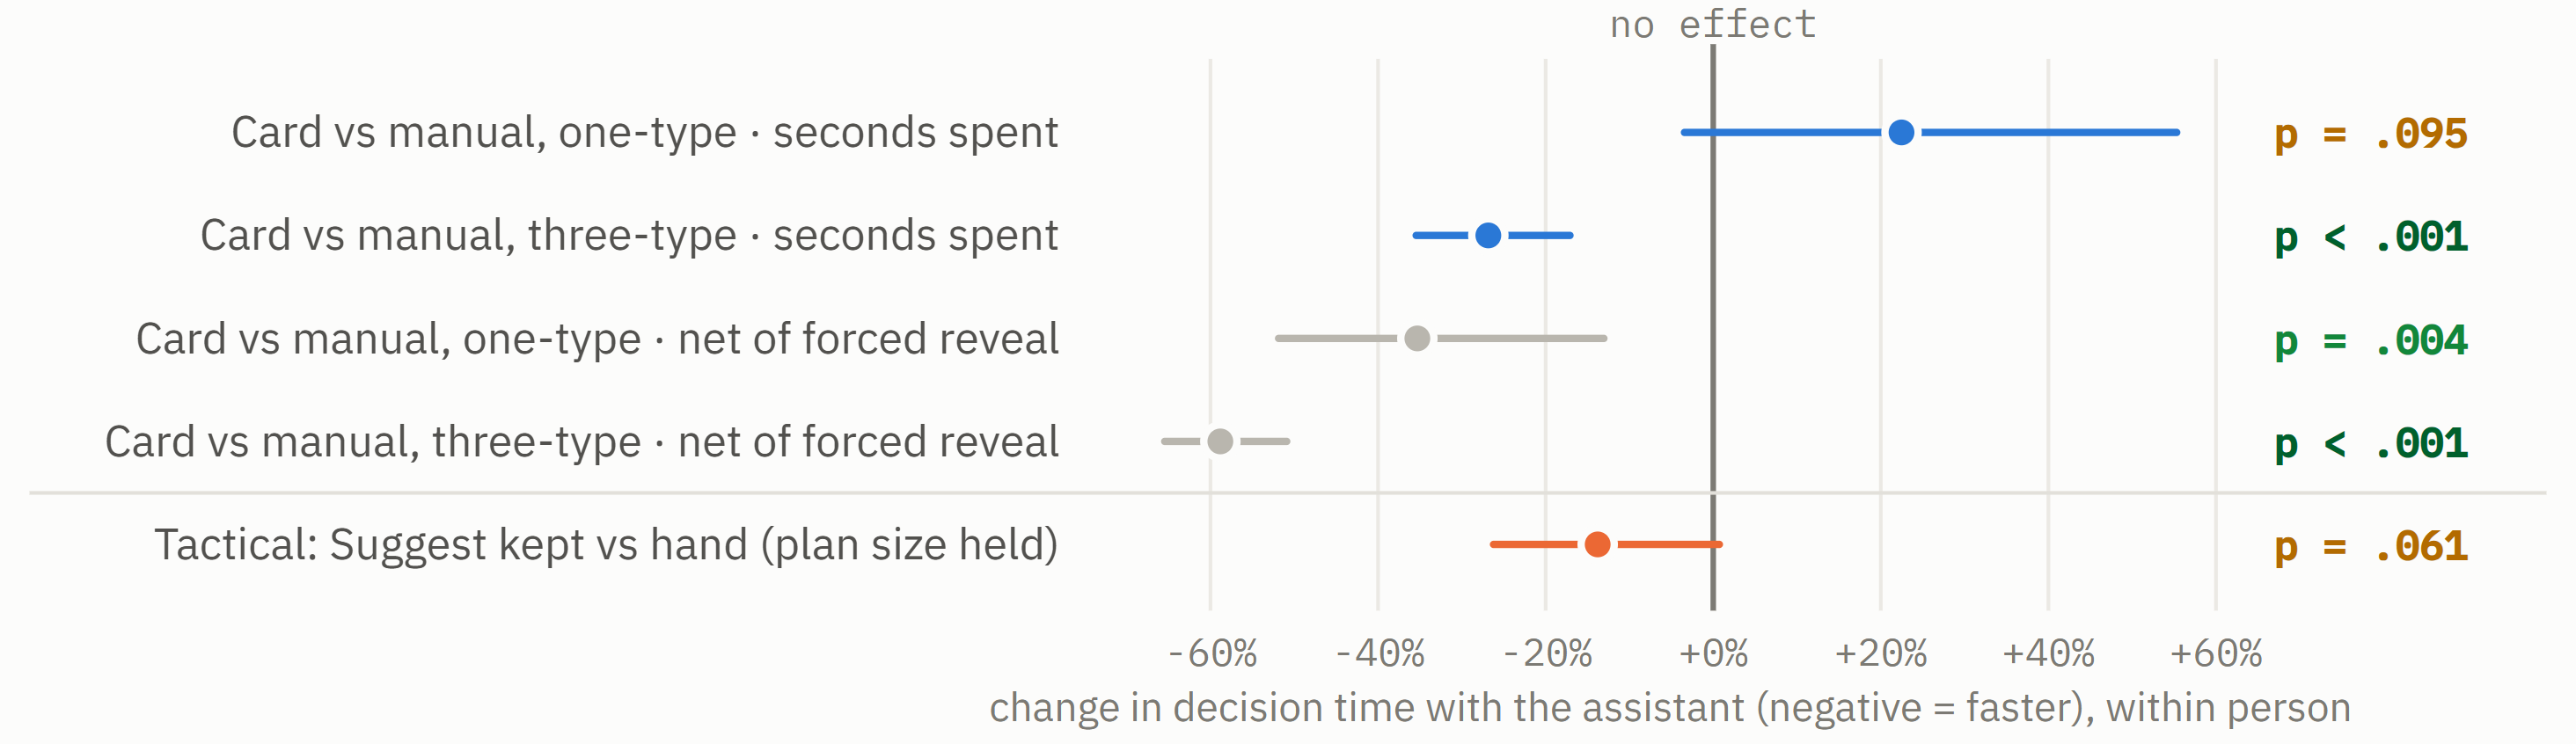
\includegraphics[width=\linewidth,height=0.55\textheight,keepaspectratio]{figs/results/f-size-decides__speed-model__main.png}
\caption{\textbf{The speed difference as estimates}}
\label{fig:res:size-decides:speed-model}
\end{figure}

\paragraph*{Method.} {\small As in the section above. Each row is a within-person \% change in decision time with its 95\% interval.}

\clearpage

\subsubsection{The exception that proves the rule: the people who call the assistant slow}\label{sec:res:size-decides:slow}

\noindent \passtag{extra: may make it in}

\noindent \regtext{Six people complain that the assistant is slow (C06: P06, P15, P16, P26, P27, P29). On every measure the two groups' intervals overlap: none of the ten differences is reliable with six people. The directions are worth a sentence, not a claim. They take cards and press Suggest at the same rate as everyone else (58\% vs 66\%; 74\% vs 76\%), and they lean \emph{towards} the size rule: they decide before the cards load more often (30\% vs 13\%, p = .055) and their three-type minus one-type gap is larger (+40 vs +19 points, p = .09). Read that way, the complaint and the rule are the same observation (the fixed wait is not worth it on small jobs), and P29 says as much. But this is a reading of six people, not a finding.} (Figure~\ref{fig:res:size-decides:slow})

\begin{figure}[H]
\centering
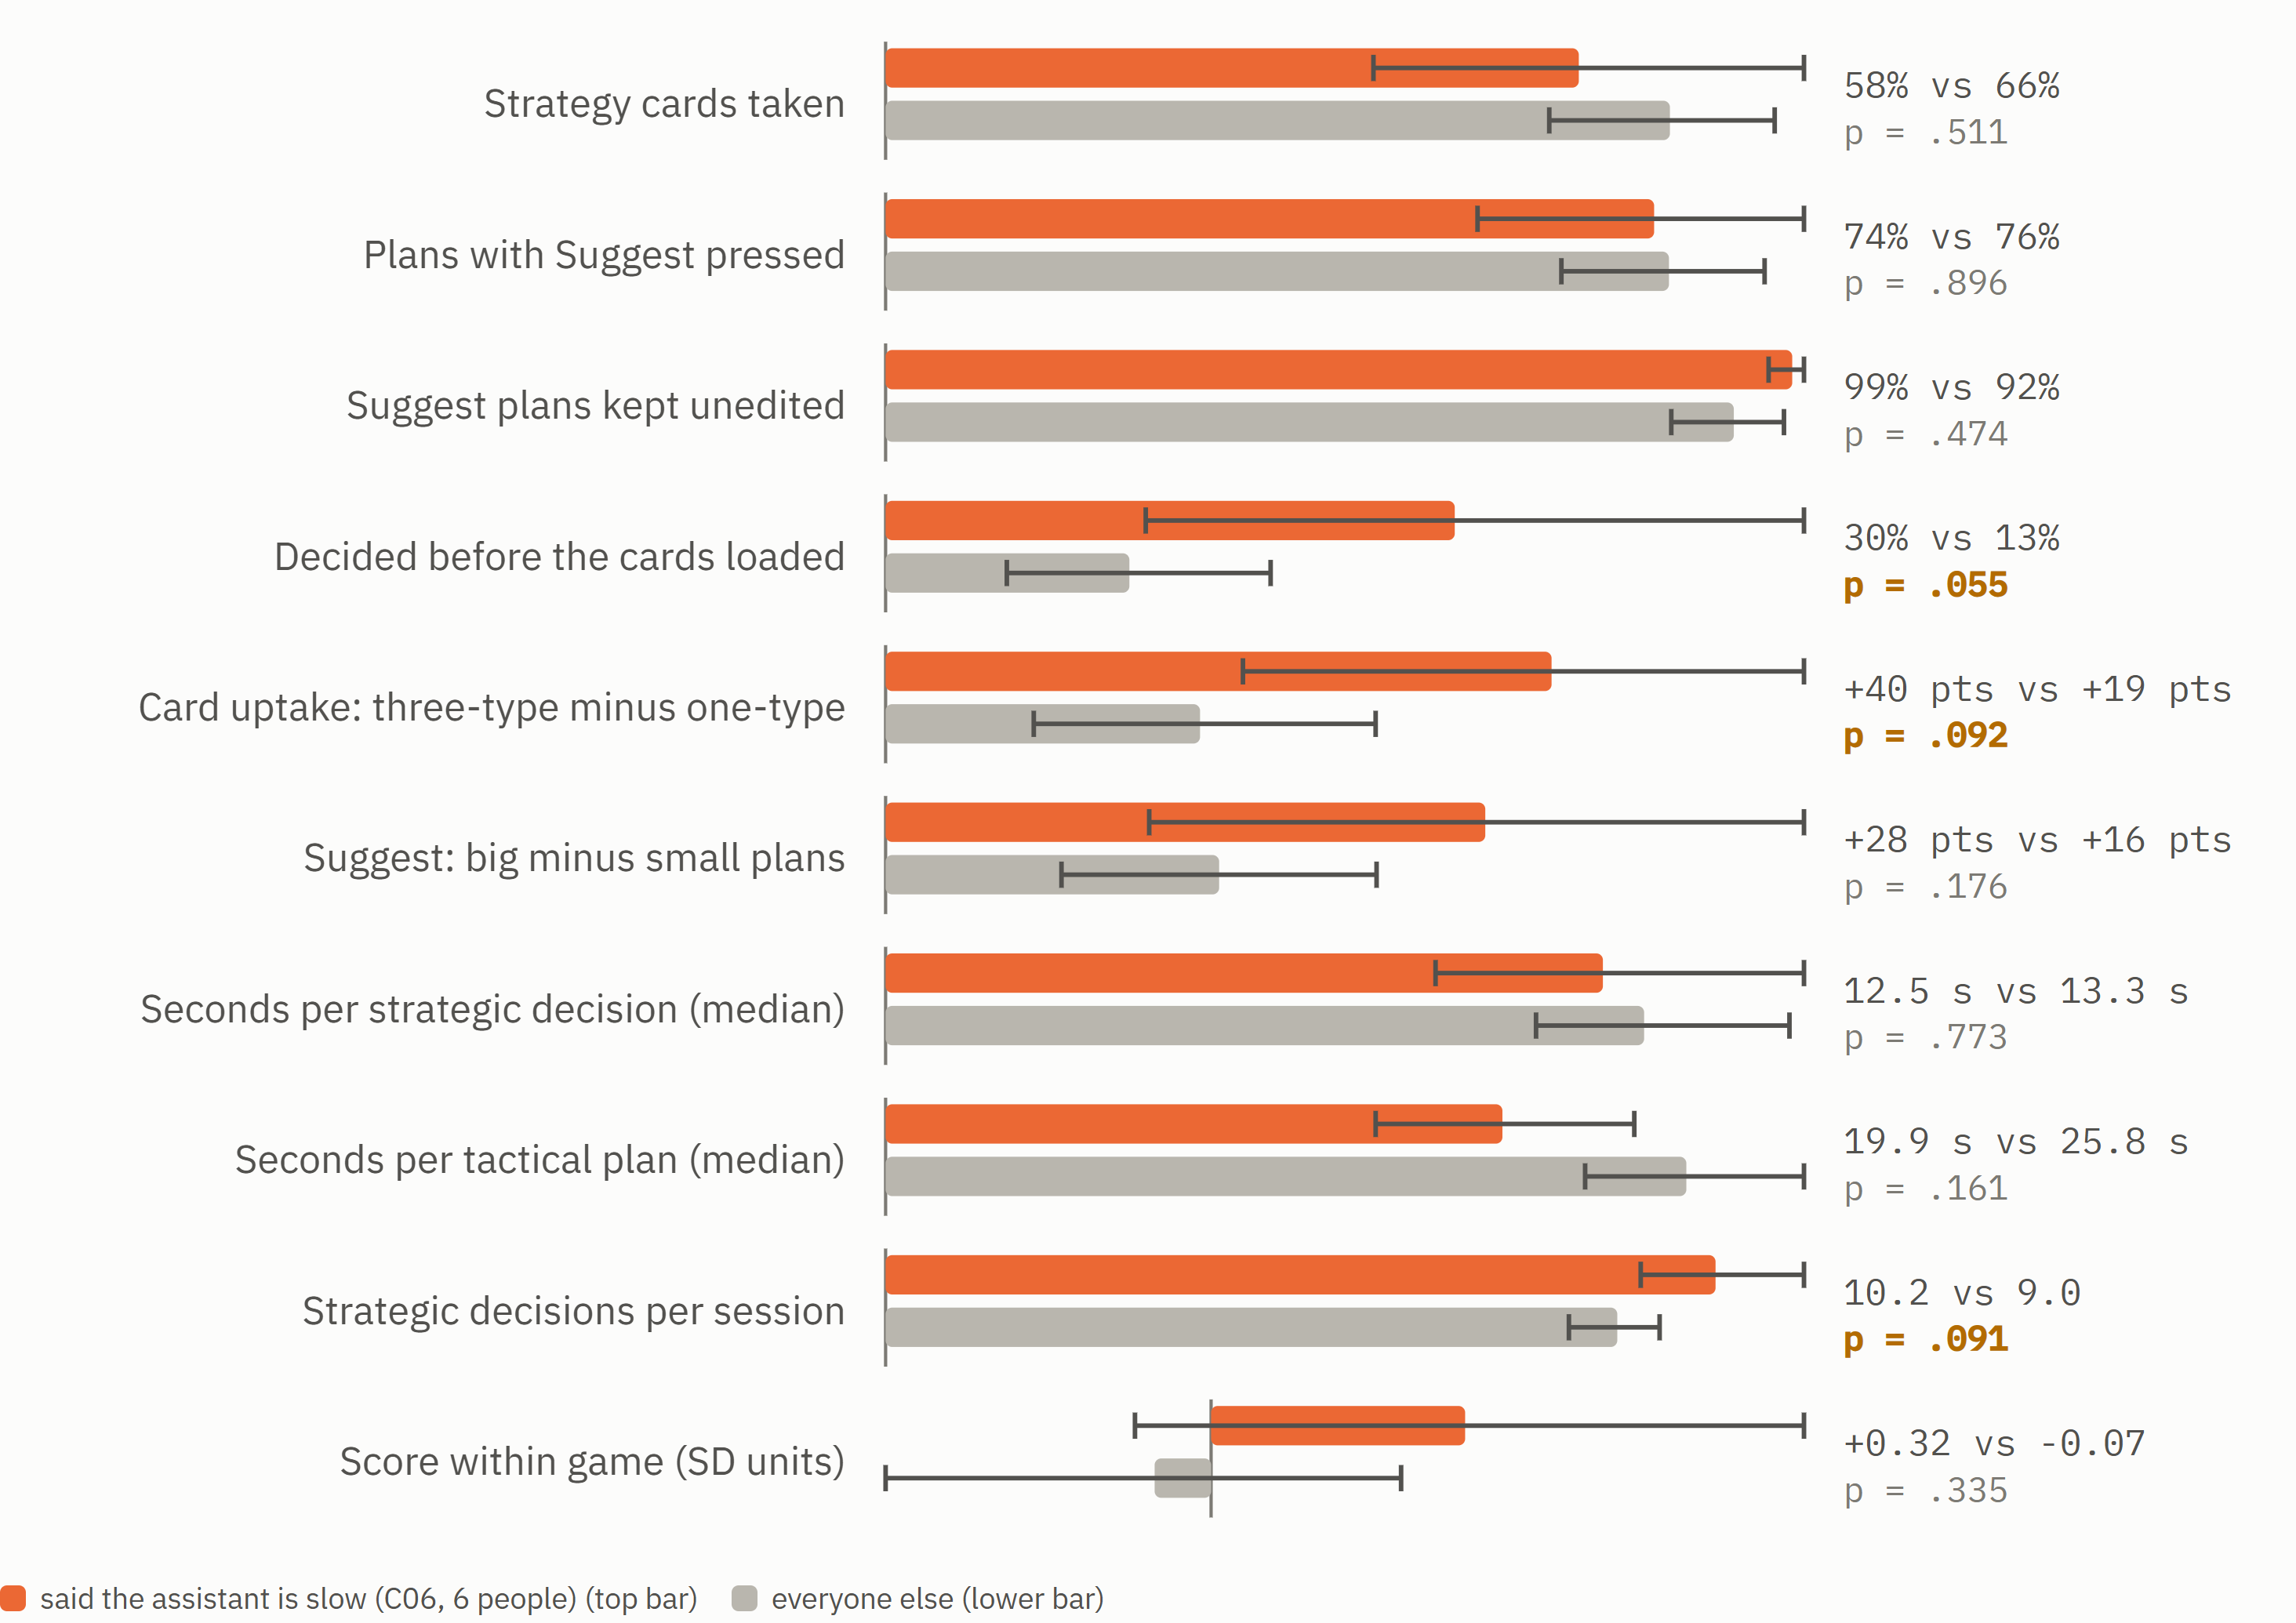
\includegraphics[width=\linewidth,height=0.55\textheight,keepaspectratio]{figs/results/f-size-decides__slow__main.png}
\caption{\textbf{The exception that proves the rule: the people who call the assistant slow}}
\label{fig:res:size-decides:slow}
\end{figure}

\paragraph*{Key numbers.}

\begin{itemize}[leftmargin=1.2em,itemsep=1pt]

\item Pre-emptive share 30\% vs 13\% (p = .055); three-type minus one-type card gap +40 vs +19 points (p = .09); decisions per session 10.2 vs 9.0 (p = .09)

\item Tactical plan time 19.9 vs 25.8 s (p = .16); score +0.32 vs $-$0.07 SD (p = .34)

\item Card uptake 58\% vs 66\% (p = .51); Suggest 74\% vs 76\% (p = .90) --- reliance itself does not differ

\end{itemize}

\paragraph*{Method.} {\small Per-person measures, averaged over the person's two sessions, for the six C06 people against the other 27. Bars are group means; whiskers are 95\% intervals from resampling people within each group. Score = session score (P01/P02 rescaled for their half task weights) standardised within each of the four games. p = two-sided permutation test (group labels reshuffled 20,000 times); 10 comparisons, uncorrected, so expect about one p below .10 by chance.}

\clearpage

\subsection{A busier moment does not push people onto the assistants --- even though they say it does (supplementary analyses)}\label{sec:sup:res:workload}

\noindent Supplement to Section~\ref{sec:res:workload}.

\subsubsection{Every way of asking it gives the same answer}\label{sec:res:workload:robust}

\noindent \passtag{numbers only}

\noindent \regtext{The within-person change in the odds of relying per extra mission waiting, under every specification tried --- including each game on its own, the heavier vs the lighter pair of games, a 'hinge' that lets the effect differ beyond the visible list, tasks waiting instead of missions, and missions that had just arrived (which the operator cannot cause). Strategic: all 13 are compatible with no change. Tactical: the main model is flat, but two of twelve variants reach p < .05 (without mission size; Strategic Heavy game 1 alone) --- a small upward lean that disappears once mission size is held fixed and is absent for the arrivals measure.} (Figure~\ref{fig:res:workload:robust})

\begin{figure}[H]
\centering
\begin{subfigure}[t]{\linewidth}
\centering
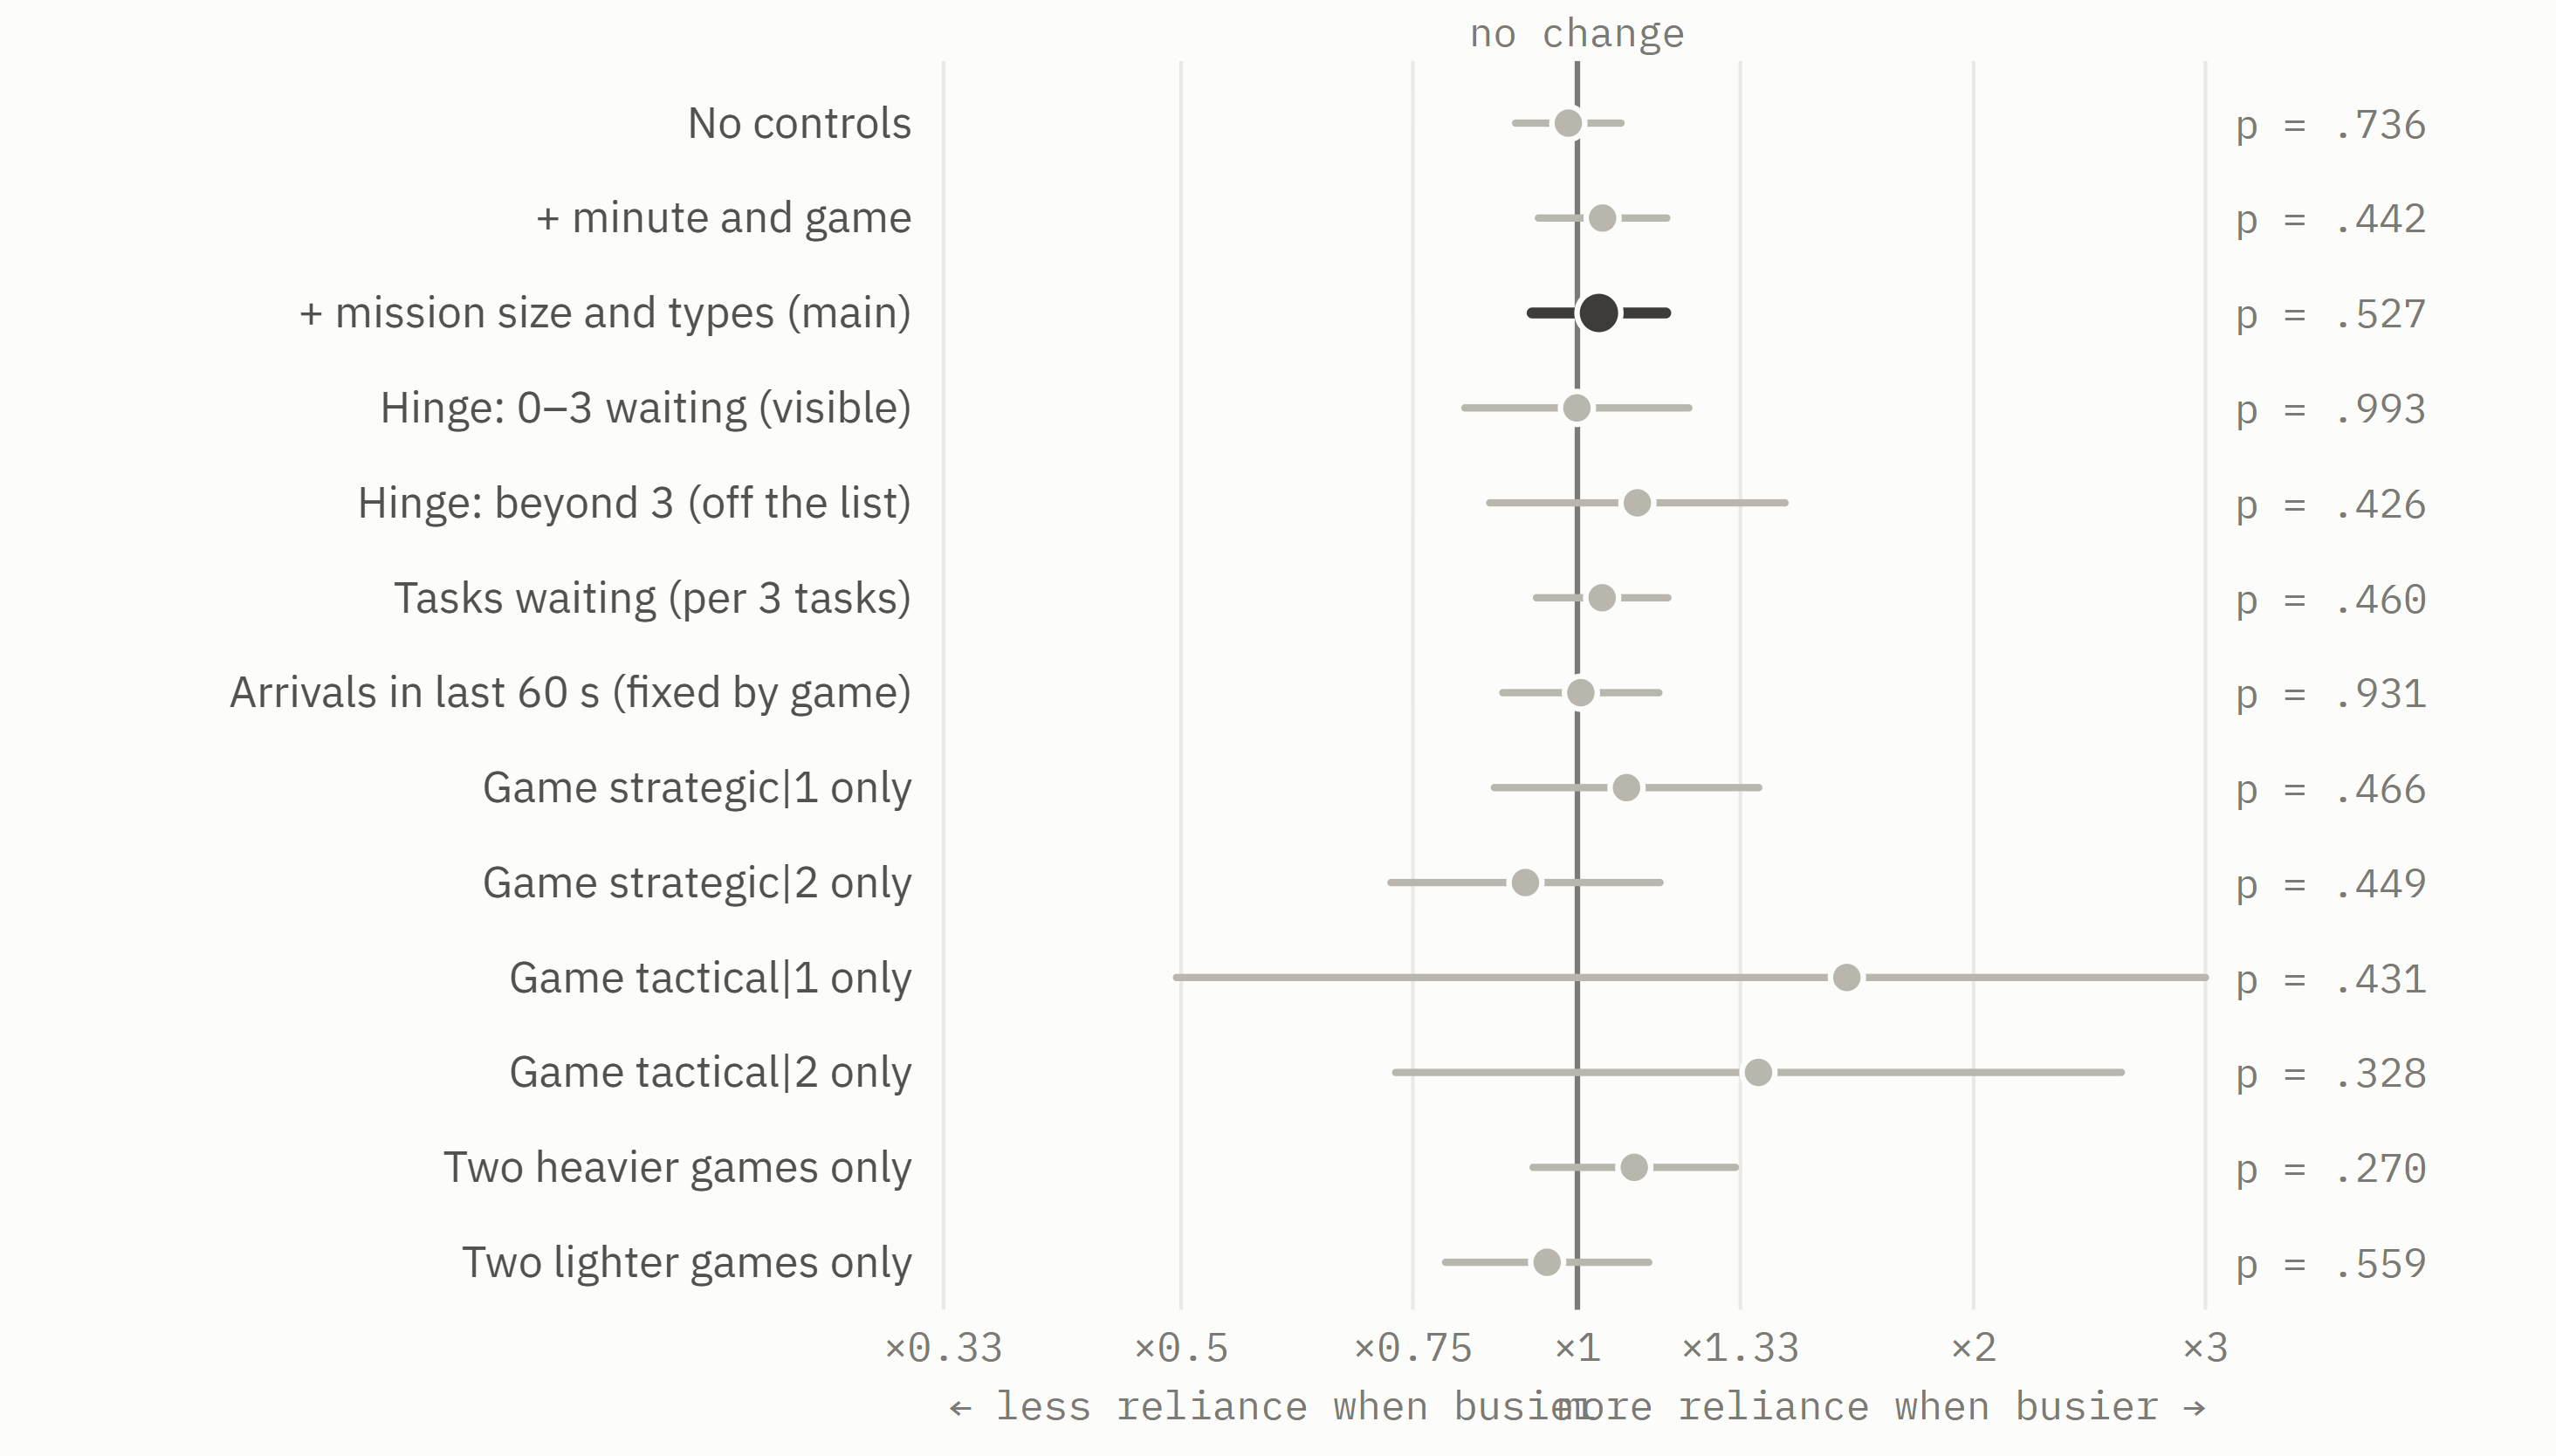
\includegraphics[width=\linewidth,height=0.23\textheight,keepaspectratio]{figs/results/f-workload__robust__strat.png}
\caption{Strategic tier.}
\label{fig:res:workload:robust:strat}
\end{subfigure}
\par\smallskip
\begin{subfigure}[t]{\linewidth}
\centering
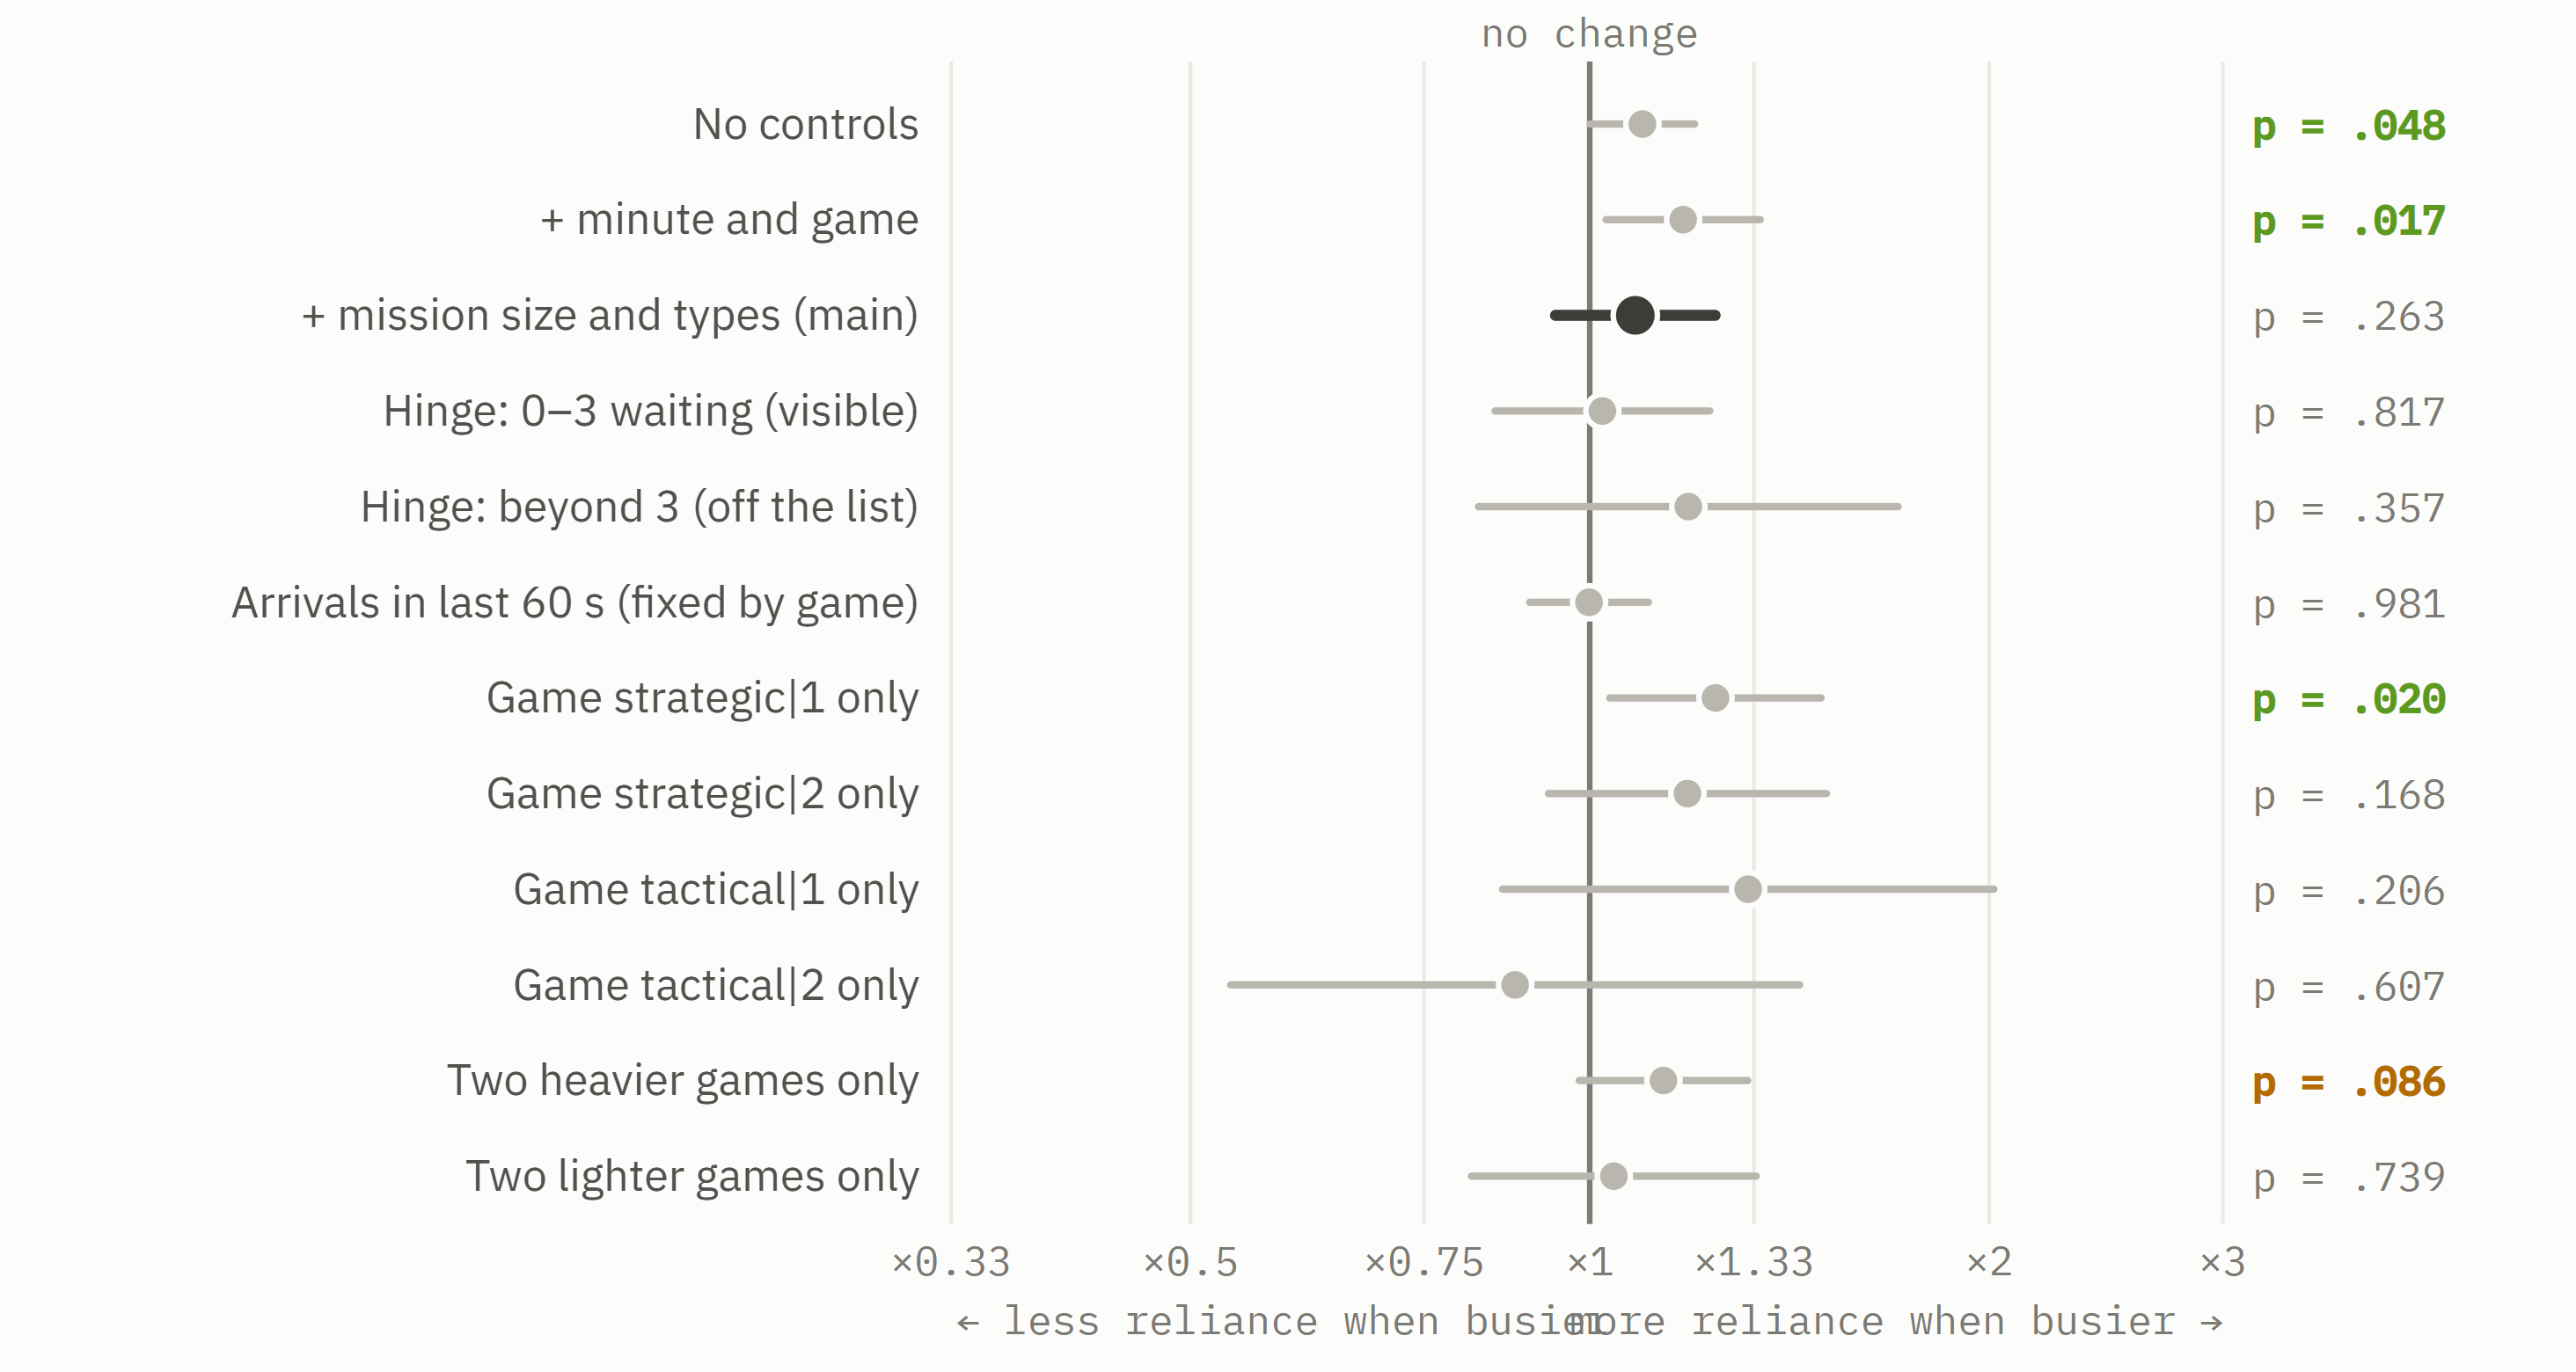
\includegraphics[width=\linewidth,height=0.23\textheight,keepaspectratio]{figs/results/f-workload__robust__tac.png}
\caption{Tactical tier.}
\label{fig:res:workload:robust:tac}
\end{subfigure}
\par\smallskip
\caption{\textbf{Every way of asking it gives the same answer}}
\label{fig:res:workload:robust}
\end{figure}

\paragraph*{Key numbers.}

\begin{itemize}[leftmargin=1.2em,itemsep=1pt]

\item Strategic main: OR 1.04 [0.92, 1.17], p = .53 per extra mission waiting; range across 13 specs 0.91--1.60, none p < .05.

\item Strategic hinge: 0--3 waiting OR 1.00 [0.82, 1.22]; beyond 3 OR 1.11 [0.86, 1.44] --- no change at the visible limit.

\item Tactical main: OR 1.08 [0.94, 1.24], p = .26; + minute and game only: 1.18 [1.03, 1.34], p = .017; arrivals in last 60 s: 1.00 [0.90, 1.11].

\item Heavier games only (Strategic Heavy 1, Tactical Heavy 2): strategic 1.10 [0.93, 1.32], tactical 1.14 [0.98, 1.32].

\end{itemize}

\paragraph*{Method.} {\small GEE logistic regression (decisions clustered within person, bias-reduced standard errors). 'Within person' means the queue is centred on that person's own average, so the estimate compares a person when busier with the same person when less busy; their average queue is kept as a separate term. 'Main' adds mission size, tasks, drone types, minute and game. An odds ratio of 1.04 means the odds of taking a card are 4\% higher per extra mission waiting. To make the interval concrete: at the main model's upper limit (1.17) uptake would rise from 65\% at 0 waiting to 80\% at 5; at its lower limit (0.92) it would fall to 56\%. So the data rule out a large effect but not a modest one either way.}

\clearpage

\subsubsection{Said vs did: the people who said they hand over when busy}\label{sec:res:workload:said-did}

\noindent \passtag{numbers only}

\noindent \regtext{Nine operators (P05, P06, P11, P18, P20, P25, P32, P33, P35) said, unprompted, that they lean on the assistant more when busy, overwhelmed or rushed. Each dot is one person's own slope: how much their (adjusted) reliance changed per extra mission waiting. If what they said described what they did, the red group would sit clearly right of zero. It does not: on average they move about +2 points per extra mission, not distinguishable from zero or from the other 24 people. Their claim usually compared sessions ('the first one was so fast I used it a lot') --- so the second view checks that version: reliance in their heavier game minus their lighter game. Again no difference.} (Figure~\ref{fig:res:workload:said-did})

\begin{figure}[H]
\centering
\begin{subfigure}[t]{\linewidth}
\centering
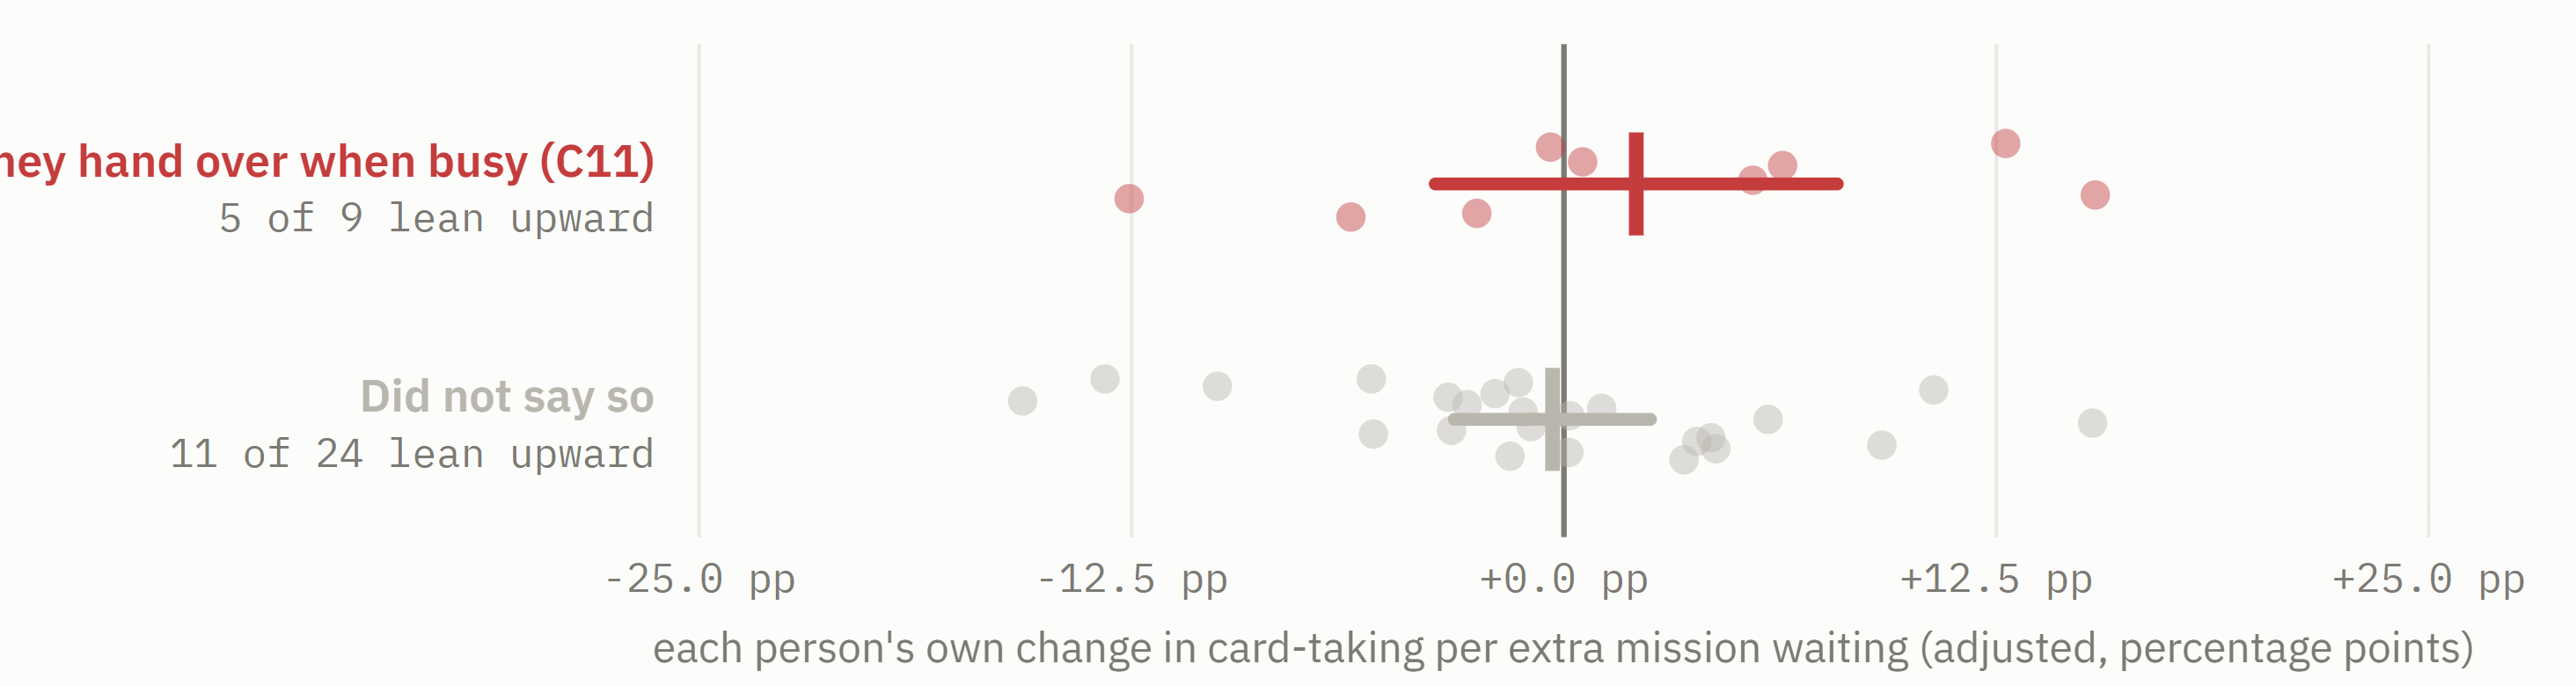
\includegraphics[width=\linewidth,height=0.23\textheight,keepaspectratio]{figs/results/f-workload__said-did__strat.png}
\caption{Strategic tier, moment to moment.}
\label{fig:res:workload:said-did:strat}
\end{subfigure}
\par\smallskip
\begin{subfigure}[t]{\linewidth}
\centering
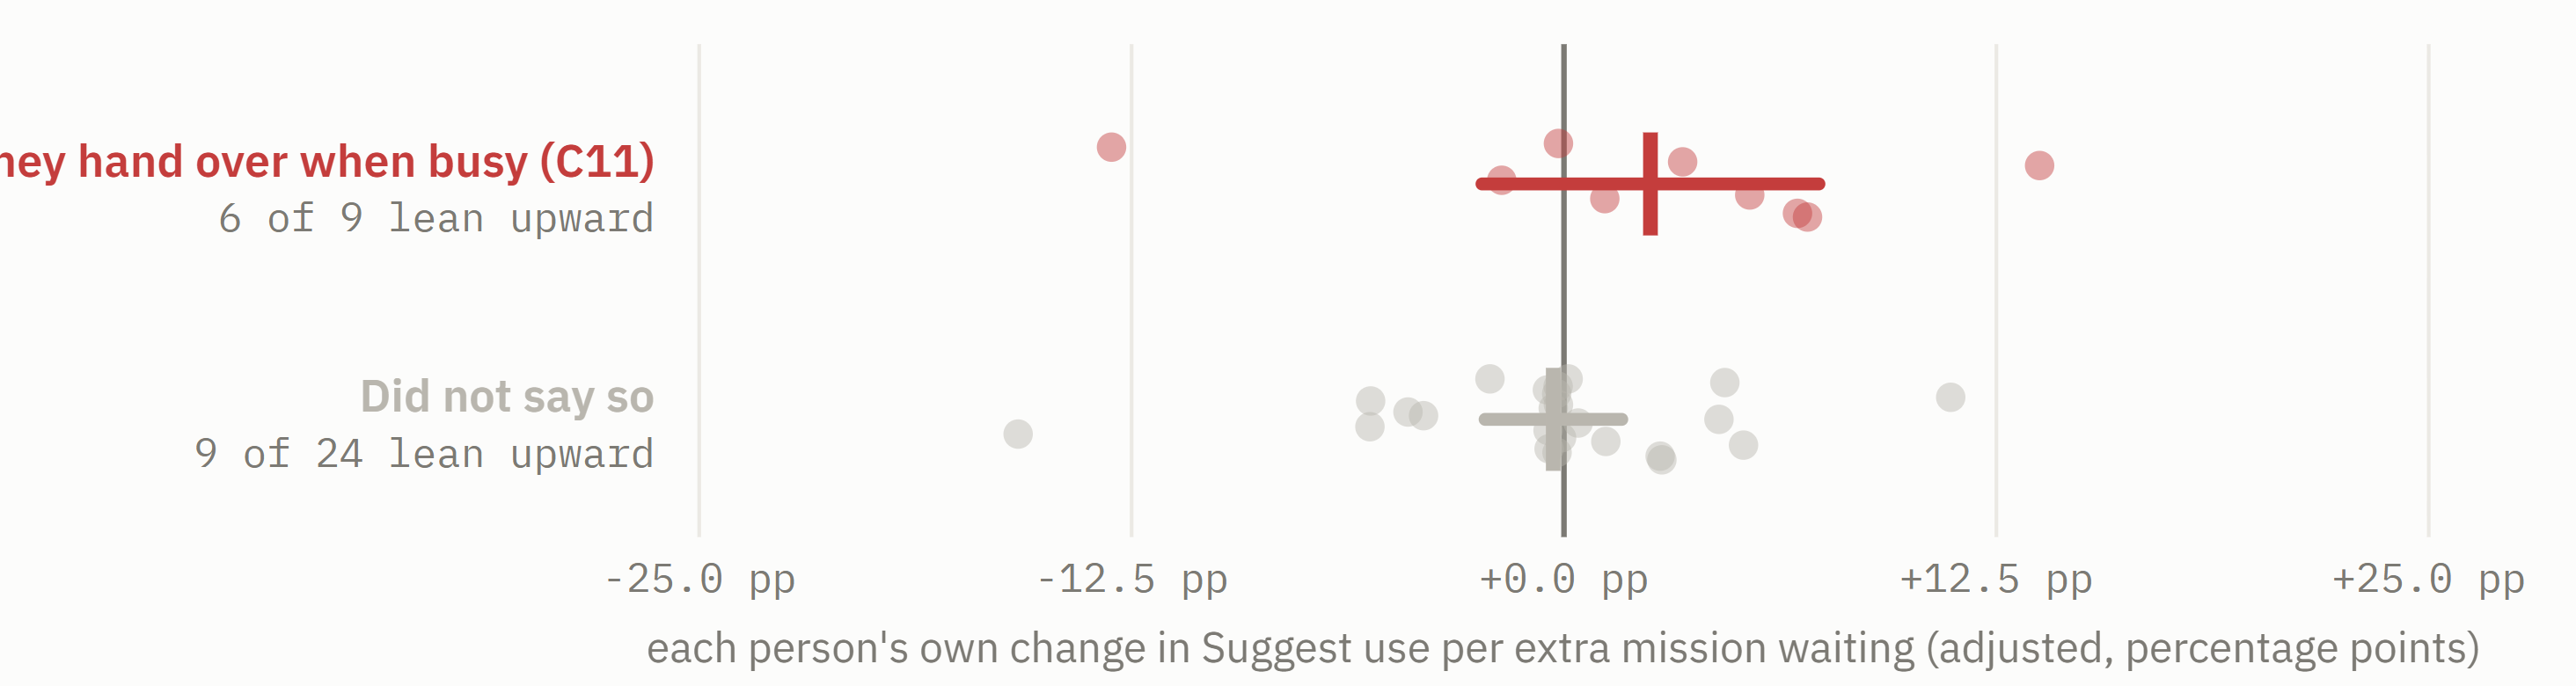
\includegraphics[width=\linewidth,height=0.23\textheight,keepaspectratio]{figs/results/f-workload__said-did__tac.png}
\caption{Tactical tier, moment to moment.}
\label{fig:res:workload:said-did:tac}
\end{subfigure}
\par\smallskip
\caption{\textbf{Said vs did: the people who said they hand over when busy}}
\label{fig:res:workload:said-did}
\end{figure}

\paragraph*{Key numbers.}

\begin{itemize}[leftmargin=1.2em,itemsep=1pt]

\item Strategic slopes: said +2.1 pp per extra mission (5 of 9 upward) vs not said $-$0.3 pp (11 of 24 upward); p = .41.

\item Tactical slopes: said +2.5 pp (6 of 9 upward) vs $-$0.3 pp (9 of 24); p = .09 --- the closest thing to support, and not significant.

\item Queue $\times$ said interaction: strategic OR 1.13 [0.83, 1.53] p = .44; tactical 1.18 [0.91, 1.53] p = .20. Within the 'said' group alone the queue OR is 1.03 (strategic) and 0.97 (tactical).

\item Heavier minus lighter game, adjusted: said +3.8 pp strategic, +1.5 pp tactical; everyone $-$1.1 / +1.2 pp; all intervals span zero.

\end{itemize}

\paragraph*{Method.} {\small \textbf{Moment to moment:} for each person with 6+ decisions and some spread in queue depth, a straight line through their (observed $-$ expected) values against queue depth; the slope is in percentage points per extra mission waiting. Groups compared with a Mann--Whitney test; also tested as a queue $\times$ 'said' interaction in the GEE above. \textbf{Busier session:} the four games' load measured by total drones demanded per session (Tactical Heavy 2: 115; Strategic Heavy 1: 89; Strategic Heavy 2: 88; Tactical Heavy 1: 63); for each person, their mean (observed $-$ expected) in the heavier of their two games minus the lighter. With 9 people in the 'said' group, only a large difference could have been detected --- this is absence of evidence for the claim, and the point estimates are small.}

\clearpage

\subsubsection{In play: overload talk comes at slightly busier moments, reliance does not follow}\label{sec:res:workload:spoken}

\noindent \passtag{extra: may make it in}

\noindent \regtext{Using the narration recorded during play (30 people, 60 sessions), we found every moment someone said an overload-type phrase ('too many', 'can't keep up', 'oh no', 'struggling'\ldots{}): 51 moments from 24 people. All nine of the 'said' group produced at least one. At those moments slightly more missions were waiting than at a random utterance (2.4 vs 2.1; p = .09) --- so what people feel as overload is weakly tied to the queue. But in the minute either side, their card-taking and Suggest use were exactly what their missions and habits predict. The felt pressure is real enough; it just does not turn into handing work over.} (Figure~\ref{fig:res:workload:spoken})

\begin{figure}[H]
\centering
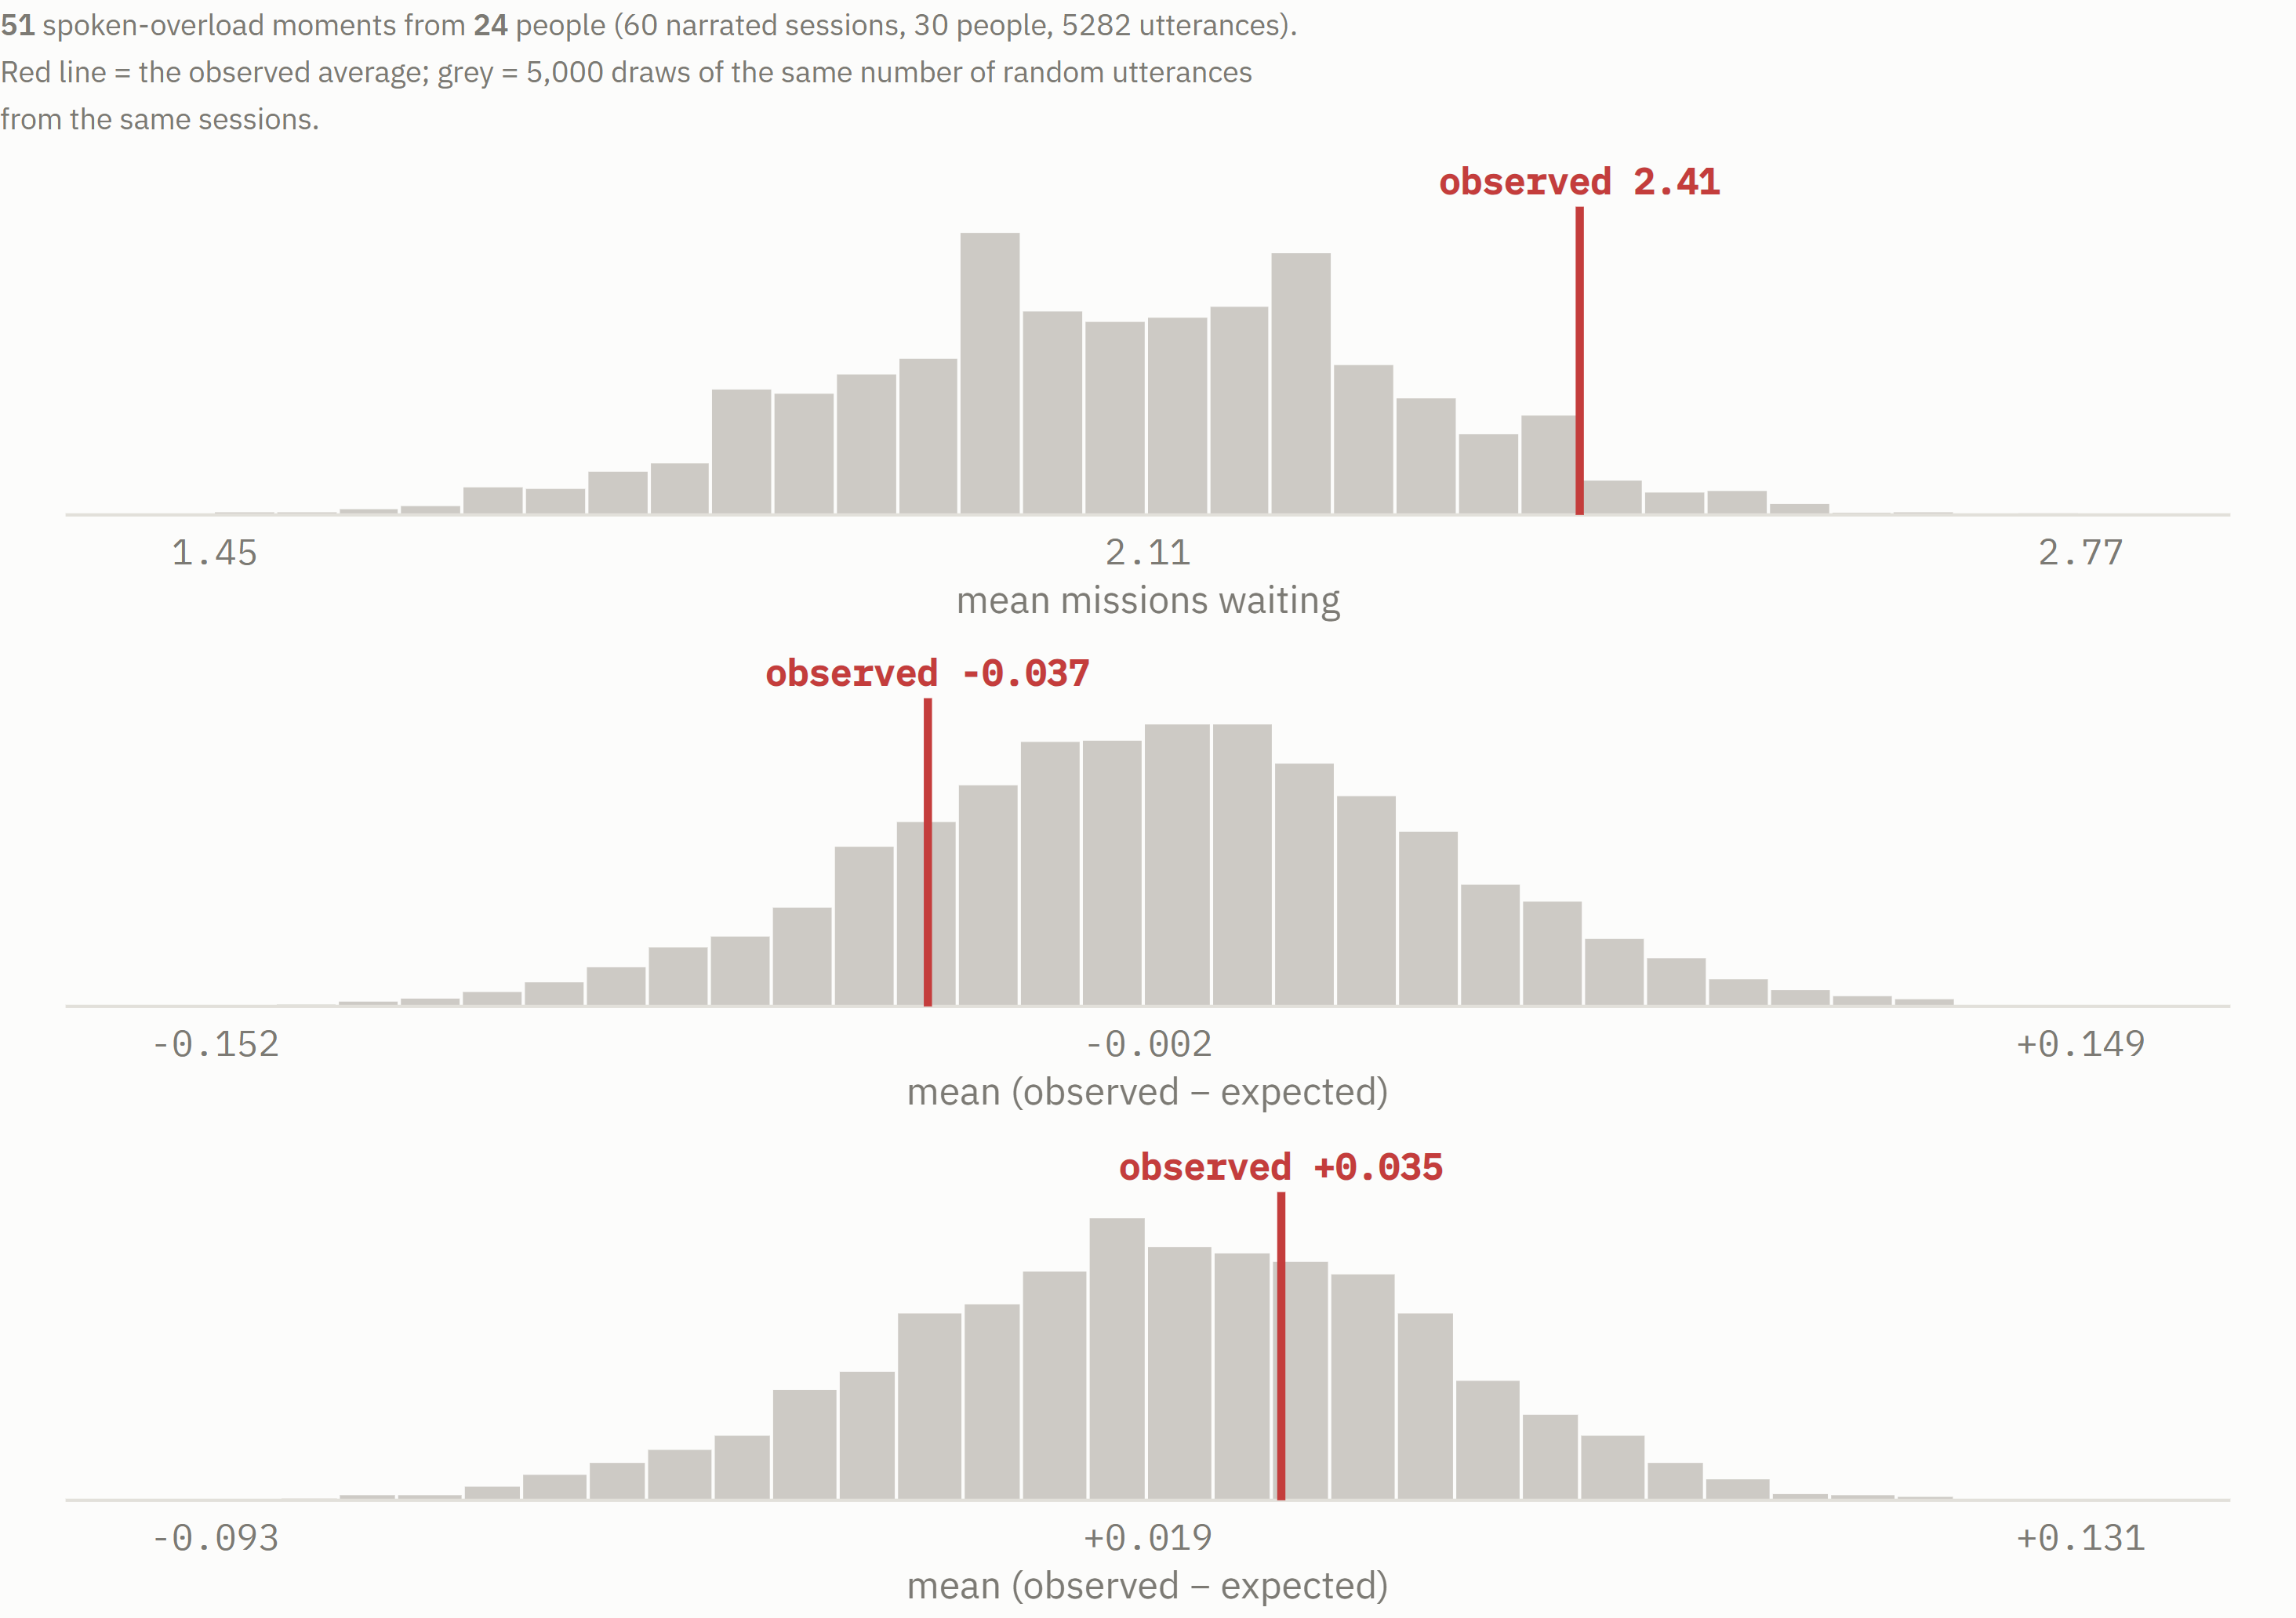
\includegraphics[width=\linewidth,height=0.55\textheight,keepaspectratio]{figs/results/f-workload__spoken__main.png}
\caption{\textbf{In play: overload talk comes at slightly busier moments, reliance does not follow} Top: missions waiting at the overload moments; middle: strategy cards taken within $\pm$60\,s (observed $-$ expected); bottom: Suggest pressed within $\pm$60\,s (observed $-$ expected). Red line = observed mean; grey = 5,000 draws of the same number of random utterances from the same sessions.}
\label{fig:res:workload:spoken}
\end{figure}

\paragraph*{Key numbers.}

\begin{itemize}[leftmargin=1.2em,itemsep=1pt]

\item Missions waiting at overload moments 2.41 vs 2.09 at random utterances (95\% of random draws 1.71--2.45), p = .09.

\item Card-taking within $\pm$60 s: $-$3.7 pp vs expected (random utterances +0.1), p = .38. Suggest: +3.5 pp (random +2.1), p = .65.

\item 16 of the 51 moments came from the 9 people coded C11; 35 from others.

\end{itemize}

\paragraph*{Method.} {\small Phrase list fixed in round 2 (before any behaviour was looked at), applied to the transcript of each session window (from segments.json; utterances 20 s apart merged into one moment). For each moment: missions waiting at that second (rebuilt from the log), and the mean (observed $-$ expected) of strategic decisions and tactical plans started within $\pm$60 s. Null: the same number of utterances per session drawn at random from ALL that session's speech, 5,000 times --- so the comparison is 'overload talk' vs 'any talk', in the same people and sessions. Caveats: no speaker separation (researcher speech is in the transcripts); in round 2 about half of matched phrases were genuine stress on reading; alignment uses file times for 24 of 30 people ($\pm$2 s).}

\clearpage

\subsection{The dip in strategy-card use belongs to the people who later said they noticed the illogical card, early in the session; it shows up whether or not they had met that card yet (supplementary analyses)}\label{sec:sup:res:flaw-odd}

\noindent Supplement to Section~\ref{sec:res:flaw-odd}.

\subsubsection{Strategic flaws are visible; tactical flaws are hidden}\label{sec:res:flaw-odd:visibility}

\noindent \passtag{numbers only}

\noindent \regtext{Neither assistant had errors injected for anyone analysed (the $\varepsilon$ manipulation ran only for the excluded P09). Each tier still has a natural flaw. On the \textbf{strategic} side, it is the illogical extra drone type. It sits on the card face next to the mission's own requirements, everyone saw it, and 12 people mentioned it in debrief or interview (15 counting in-play remarks). On the \textbf{tactical} side, it is the wrong refusal: Suggest answers 'No workable plan' when a fix existed using a drone busy on another task. To the operator it looks exactly like a correct refusal. 14 people met one (23 wrong refusals out of 39). Four of them reacted aloud and accepted it, most saying they would have to abandon. Only P28 named the cause. Only 3 people ever described a tactical-plan flaw (C13), and just one of them had been wrongly refused. 'The strategic assistant is distrusted more' may partly be 'its mistakes are the ones you can see'.} (Figure~\ref{fig:res:flaw-odd:visibility})

\begin{figure}[H]
\centering
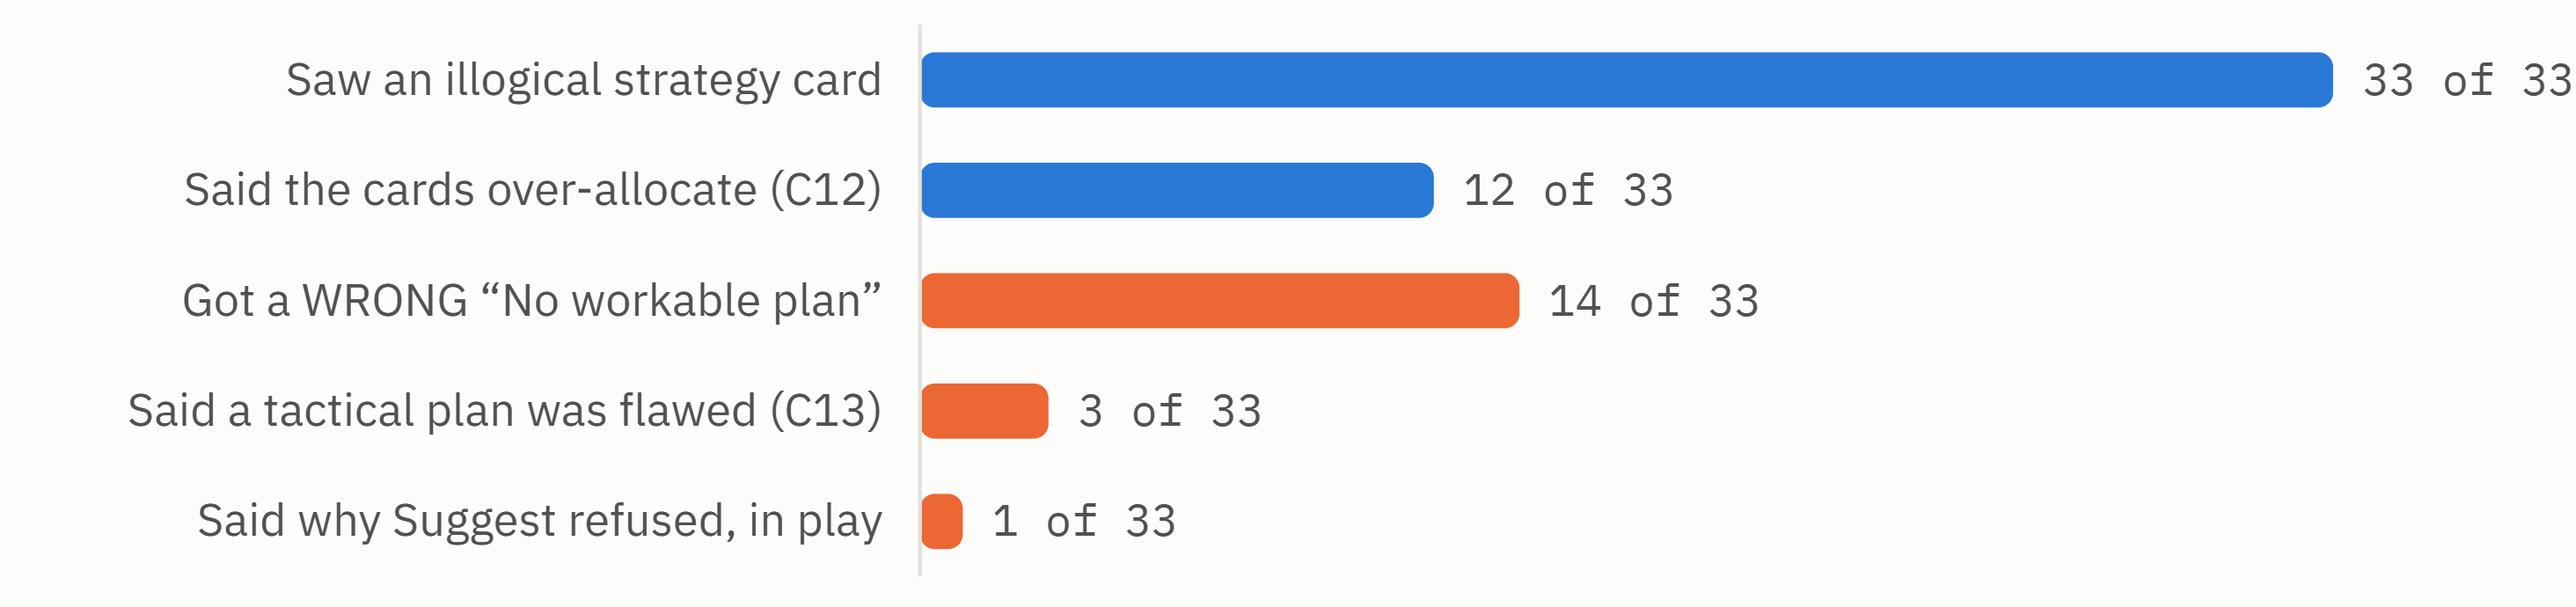
\includegraphics[width=\linewidth,height=0.55\textheight,keepaspectratio]{figs/results/f-flaw-odd__visibility__main.png}
\caption{\textbf{Strategic flaws are visible; tactical flaws are hidden}}
\label{fig:res:flaw-odd:visibility}
\end{figure}

\paragraph*{Key numbers.}

\begin{itemize}[leftmargin=1.2em,itemsep=1pt]

\item Strategic: 33 of 33 saw the illogical card (132 of 606 decisions); 12 coded C12; 15 incl. strict in-play remarks

\item Tactical: 14 of 33 got $\geq$1 wrong refusal (23 of 39 refusals); 3 coded C13, 1 of them among the 14; 4 reacted aloud to a wrong refusal, 1 named why

\end{itemize}

\paragraph*{Method.} {\small Strategic exposure: people with $\geq$1 illogical-card decision. Tactical exposure: people with $\geq$1 Suggest press in a recovery that returned 'No workable plan' or a partial plan while a fix using a busy drone existed (the 'blind' flag in h3\_recovery). Noticing: qualitative codes C12 and C13 (debrief or interview), plus the hand-coded in-play remarks (extras.SPOKEN\_STRAT / SPOKEN\_TAC), each matched to the nearest preceding Suggest press.}

\clearpage

\subsubsection{On the missions that carry the flaw, noticers stop using the cards}\label{sec:res:flaw-odd:odd-missions}

\noindent \passtag{extra: may make it in}

\noindent \regtext{This is the cleanest behavioural trace, and it is where you would expect one. On their 1st illogical-card mission, noticers took a card 47\% of the time and never-said people 56\%. With each further illogical-card mission, noticers took a card about 14 points less often. By their 4th--6th they took one \textbf{0 times in 13} (7 people), going manual instead, mostly \emph{before the cards had loaded} (62\%). Non-noticers moved the other way: by their 4th--6th they took a card 74\% of the time. Most of that was the illogical Conservative card itself (52\%), which noticers took 0 times in 13. The handover analyst's check fits this: when people build a one-type mission by hand rather than take the Conservative card, nearly all of the 'trim' is dropping the unneeded-type spares ($-$1.2 drones overall, +0.05 on the types the mission needs). So hand-builders strip out exactly what is illogical; see Section~\ref{sec:res:manual-cards}. The manual-card-error card's version (people who mention a card error go manual more on one-type missions) holds in direction. But the same people also go manual more on three-type missions, where nothing is wrong (37\% vs 22\%). The one-type-\emph{specific} part does not hold between people (interaction OR 1.12, p = .78). What is specific to the flawed missions is the \emph{trend}: noticers learn to skip the cards there.} (Figure~\ref{fig:res:flaw-odd:odd-missions})

\begin{figure}[H]
\centering
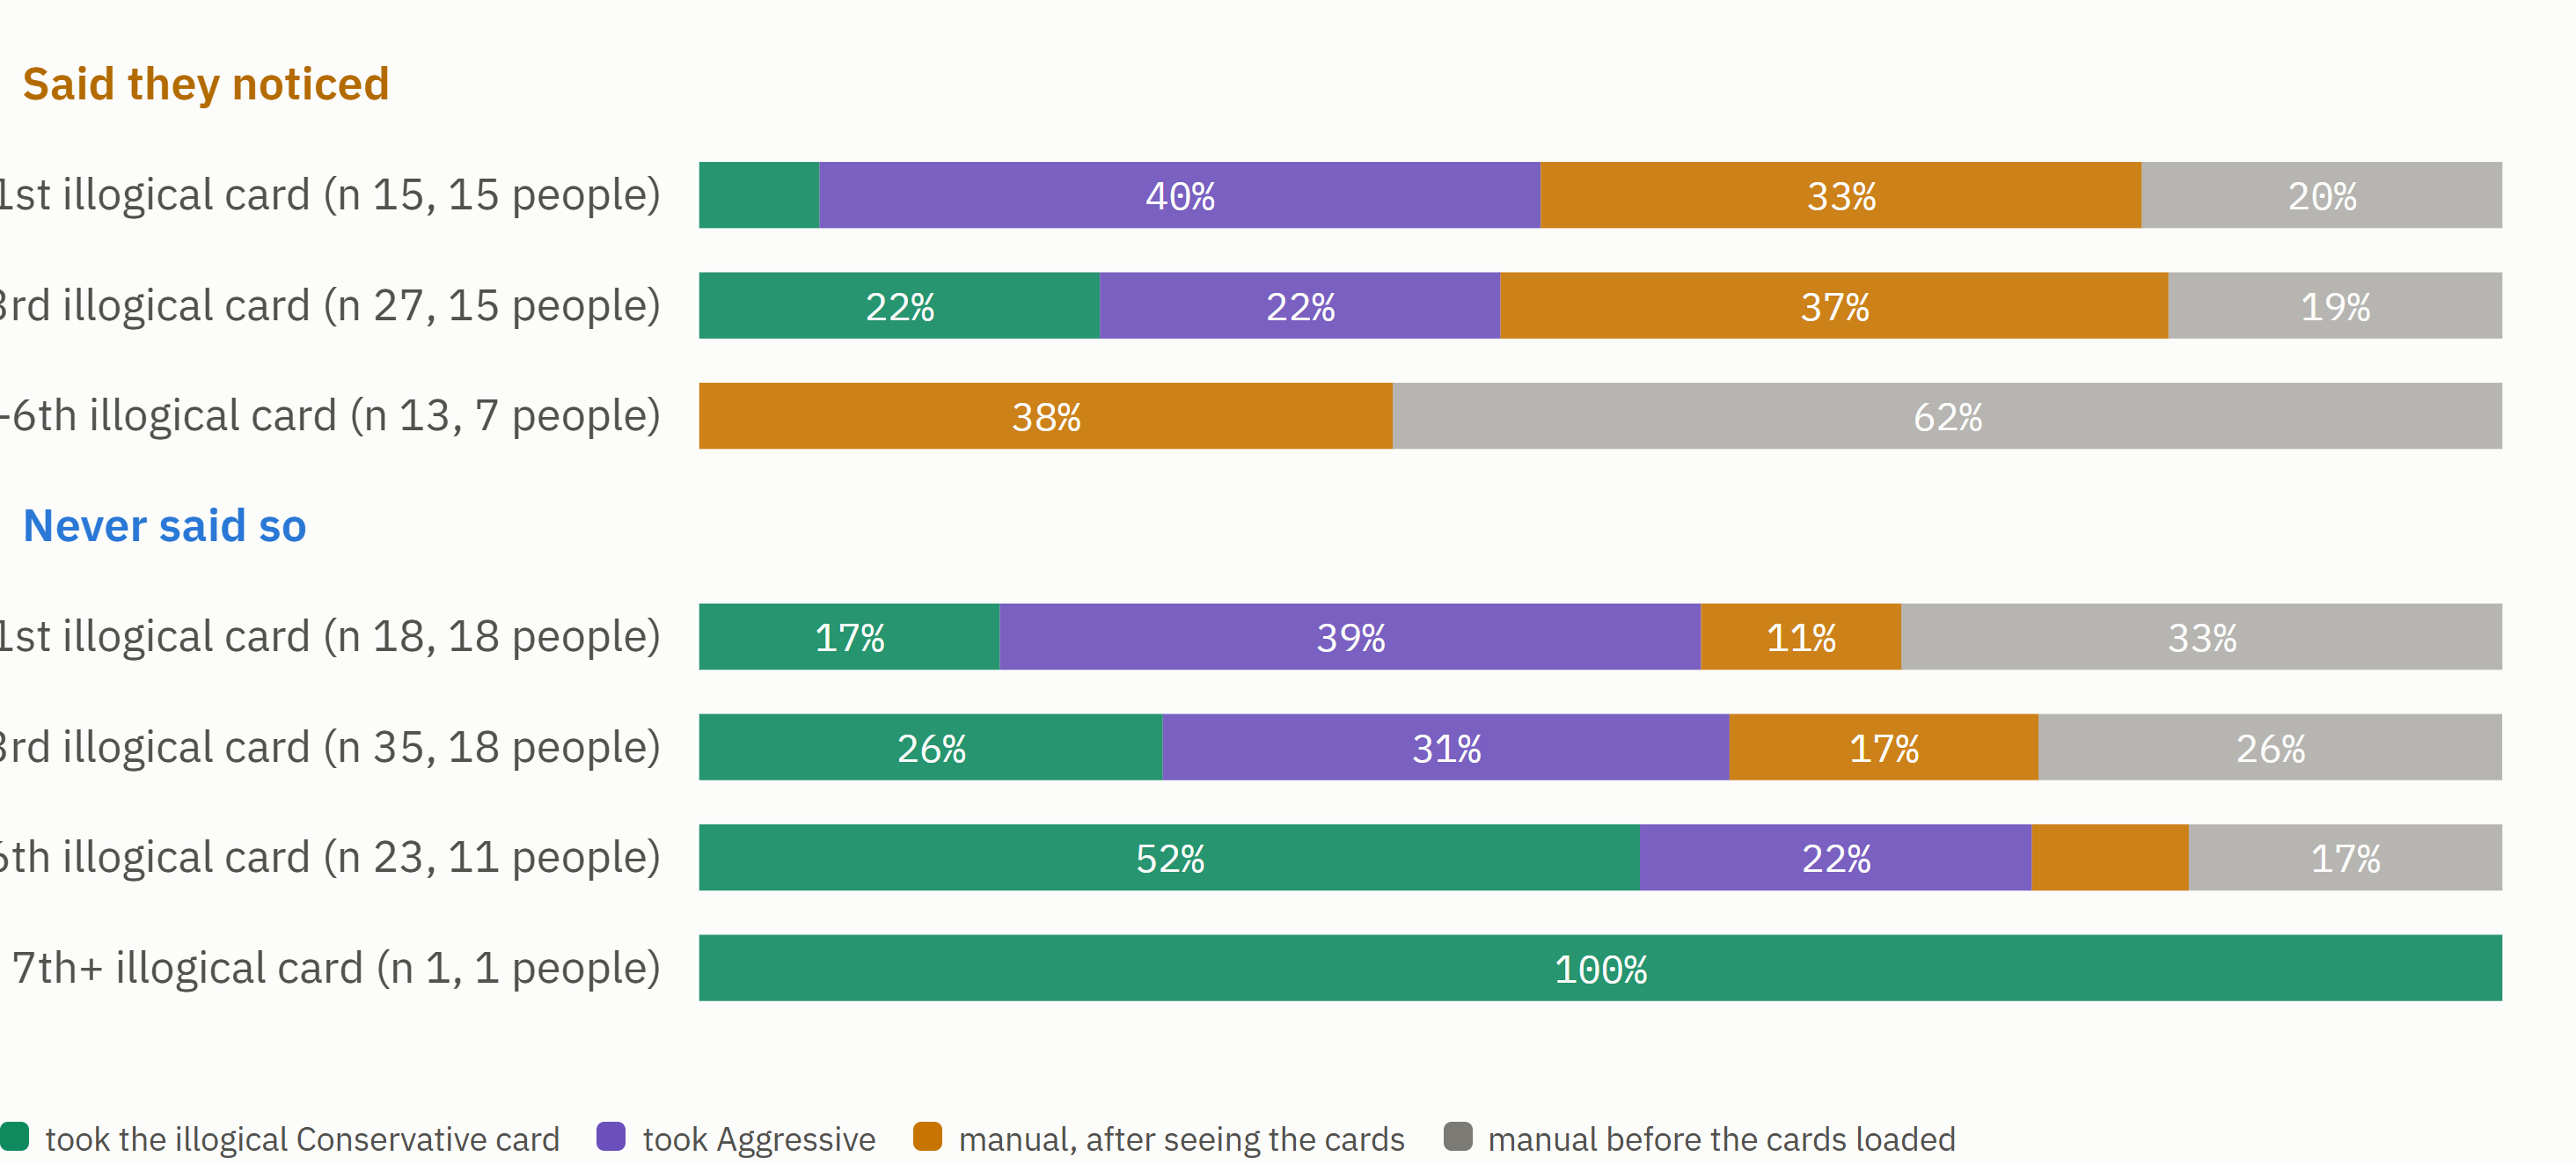
\includegraphics[width=\linewidth,height=0.55\textheight,keepaspectratio]{figs/results/f-flaw-odd__odd-missions__main.png}
\caption{\textbf{On the missions that carry the flaw, noticers stop using the cards}}
\label{fig:res:flaw-odd:odd-missions}
\end{figure}

\paragraph*{Key numbers.}

\begin{itemize}[leftmargin=1.2em,itemsep=1pt]

\item Took any card, per extra illogical card: noticers $-$13.9 points [$-$25, $-$3]; never-said +5.3 [$-$2, +12]; difference p < .001

\item Took the illogical Conservative card: noticers $-$3.5 points per card; never-said +9.3 [+1, +18]; difference p = .001

\item Manual before the cards loaded: noticers +15.4 points per card [+2, +29]; never-said $-$5.8; difference p = .012

\item 4th--6th illogical card: noticers took a card 0 of 13 (7 people); never-said 74\% of 23 (11 people), 52\% the illogical card

\item Manual on one-type missions: noticers 63\% vs 37\%, OR 2.41 [0.92, 6.32], p = .07; on three-type 37\% vs 22\%, OR 2.29, p = .06; one-type $\times$ noticed OR 1.12, p = .78

\end{itemize}

\paragraph*{Method.} {\small Rows: the 132 illogical-card decisions, numbered per person (1st, 2nd, \ldots{}). Each is coded by what happened: took the Conservative card (the illogical one), took Aggressive, manual after the cards loaded, or manual before they loaded (a pre-emptive choice that never saw the cards). Trend = a linear model of each outcome on the card's number (capped at 7) $\times$ group, with game held fixed and people clustered. The interaction p is whether the two groups' slopes differ. Between-person check (manual-card-error): manual \textasciitilde{} said + game on one-type missions, then on three-type, then the said $\times$ one-type interaction (logistic GEE, people clustered).}

\clearpage

\subsubsection{What 'expected' and 'adjusted' mean}\label{sec:res:flaw-odd:adjustment}

\noindent \passtag{numbers only}

\noindent \regtext{\textbf{Expected} is the chance a model gives that this person takes a card on this decision. It knows only what the decision was (drones, tasks and drone types the mission needed), when it was (minute of the session, whether it was a re-queued mission, how many others were waiting), which of the four games was being played, and how often \emph{this person} took cards on all their \emph{other} decisions. \textbf{Adjusted} = the group's overall rate + the average of (observed $-$ expected) at that position. In plain terms: 'how far above or below their usual self, given the mission in front of them, were people here?' The person term does most of the work (odds $\times$2.84 per unit; the model ranks takes above non-takes 81\% of the time). So 'adjusted' mostly means 'compared with that person's normal habit'. Of the mission features, only the number of drone types matters ($\times$1.51 per extra type). Because adjusted is a shifted average residual and not a probability, it can go above 100\% at a small dot that sits far above its expectation. The old not-said +2 dot read 122\% for this reason.} (Figure~\ref{fig:res:flaw-odd:adjustment})

\begin{figure}[H]
\centering
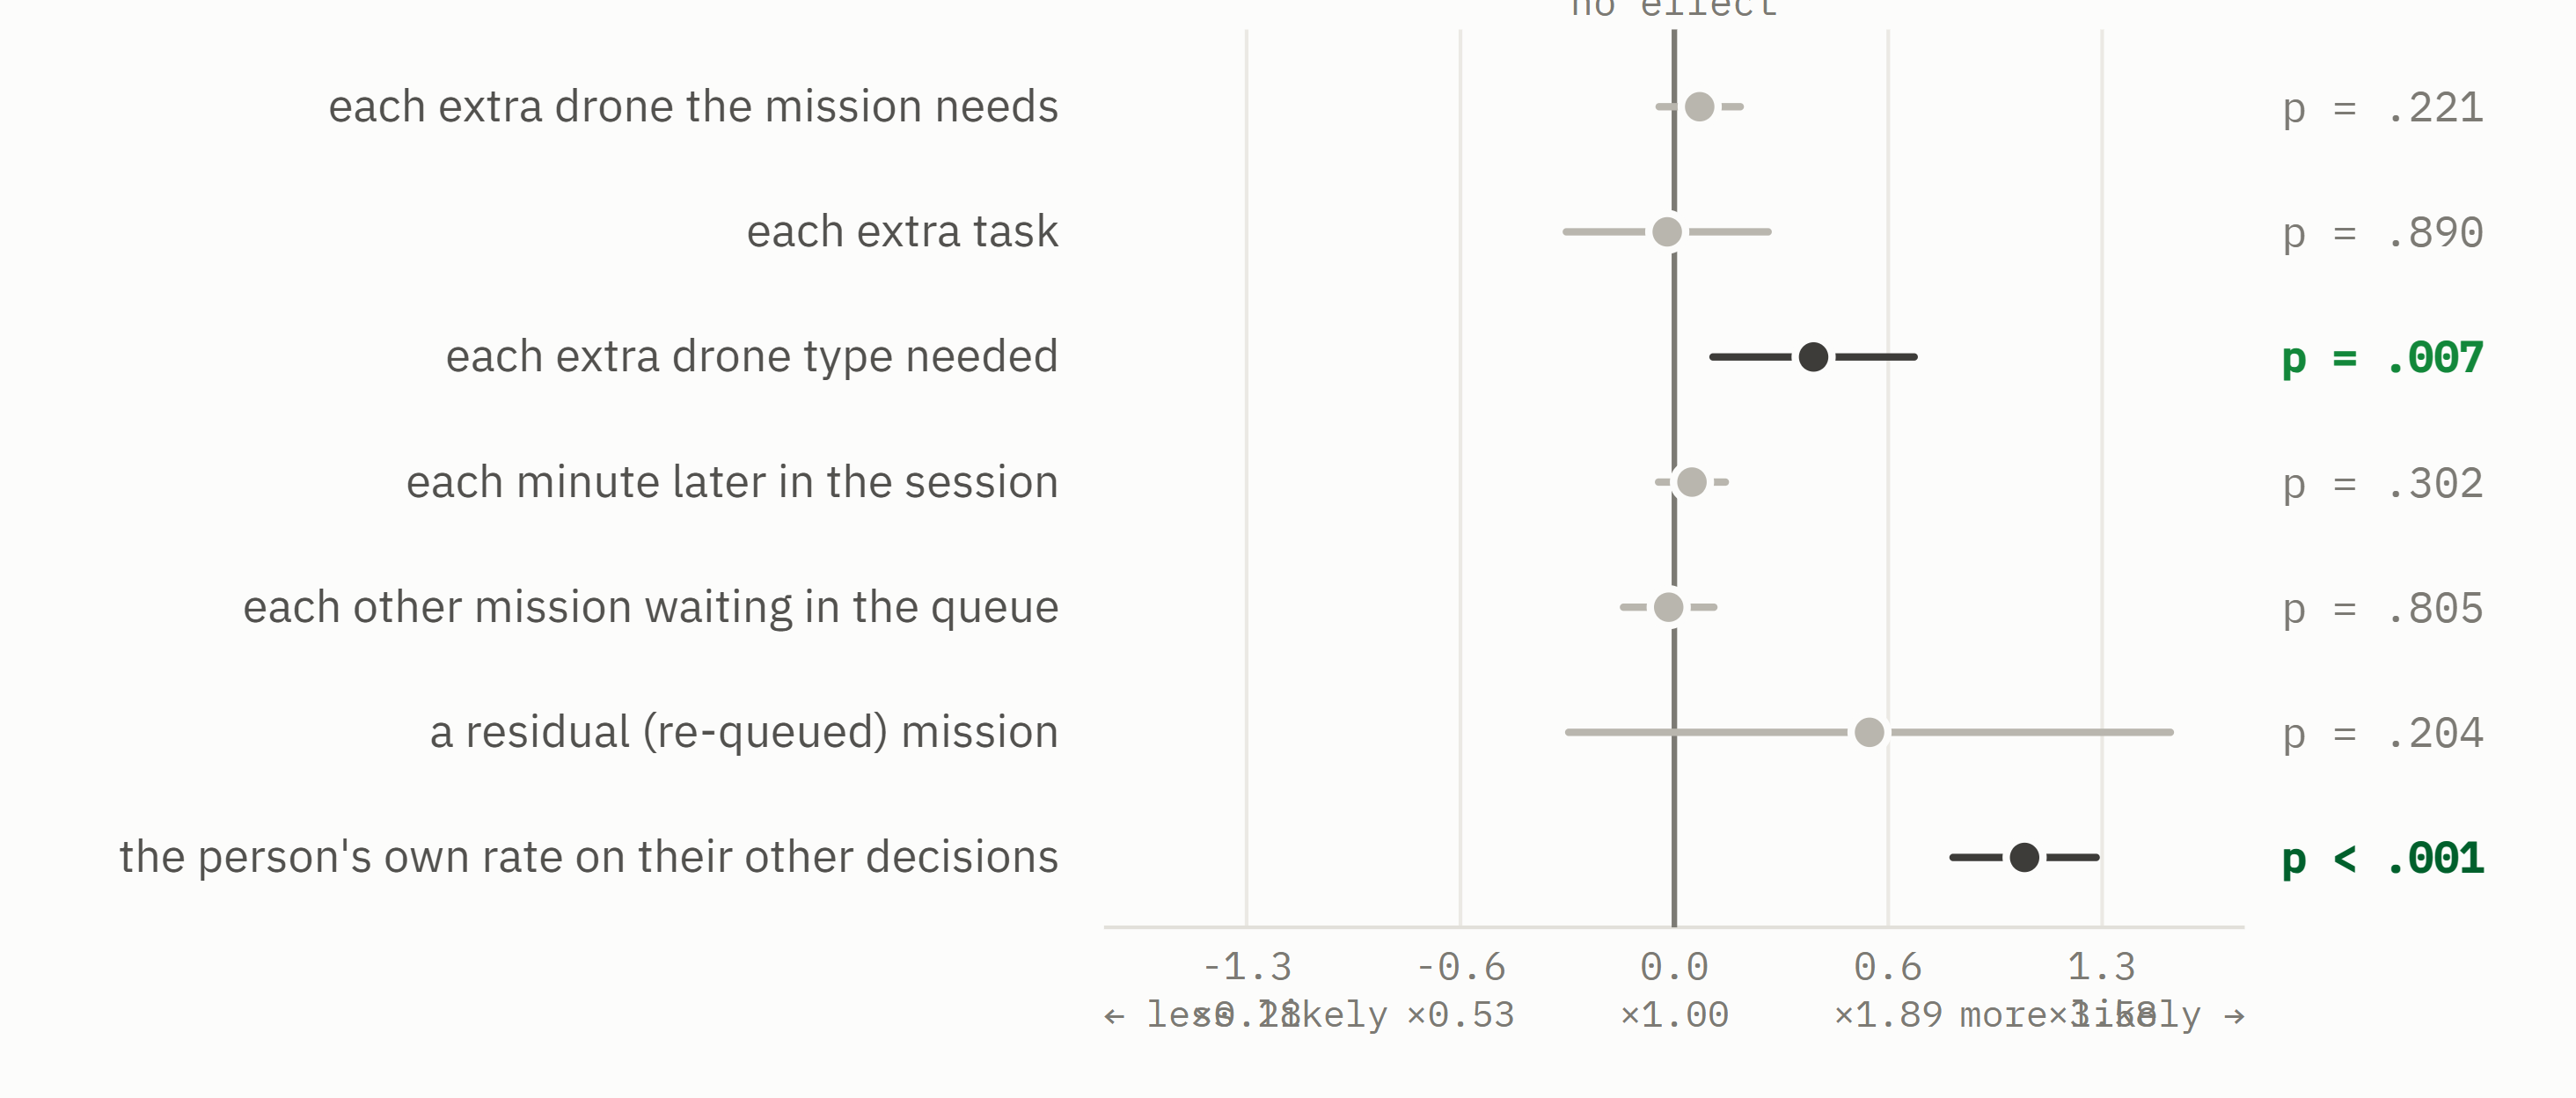
\includegraphics[width=\linewidth,height=0.55\textheight,keepaspectratio]{figs/results/f-flaw-odd__adjustment__main.png}
\caption{\textbf{What 'expected' and 'adjusted' mean}}
\label{fig:res:flaw-odd:adjustment}
\end{figure}

\paragraph*{Key numbers.}

\begin{itemize}[leftmargin=1.2em,itemsep=1pt]

\item Person's own rate elsewhere: odds $\times$2.84 [2.29, 3.51] per logit unit

\item Each extra drone type needed: $\times$1.51 [1.12, 2.04]; drones $\times$1.08, tasks $\times$0.98, minute $\times$1.05, queue $\times$0.98 (all n.s.)

\item Model ranks takes above non-takes 81\% of the time (AUC 0.81)

\end{itemize}

\paragraph*{Method.} {\small Logistic regression over all 606 decisions: took \textasciitilde{} drones + tasks + types + minute + game + queue length + residual flag + logit(person's leave-one-out rate, shrunk with +1/+2). The same specification as extras2.add\_expected; the script checks the fitted values are identical. The chart shows each term's odds ratio with a 95\% interval.}

\clearpage

\subsubsection{Abandonment by what Suggest said}\label{sec:res:flaw-odd:rates}

\noindent \passtag{numbers only}

\noindent \regtext{Every drone failure that needed the operator is one recovery episode. Grouped by what Suggest answered: a \textbf{wrong refusal} ended in abandonment 53\% of the time (9 of 17). When Suggest gave a plan it was 6\% (3 of 51), and when operators fixed things by hand without Suggest it was 13\% (9 of 69). A \textbf{correct refusal}, where no fix existed with the drones on the mission, ended in abandonment every time (11 of 11), as it should. The striking row is the first one. These were saveable missions, and the same 14 people abandoned only 6 of their 61 other attempted fixable failures. Abandonment was not their habit; the refusal is what is different. When nothing at all was tried, every failure was abandoned or left open (35 + 11).} (Figure~\ref{fig:res:flaw-odd:rates})

\begin{figure}[H]
\centering
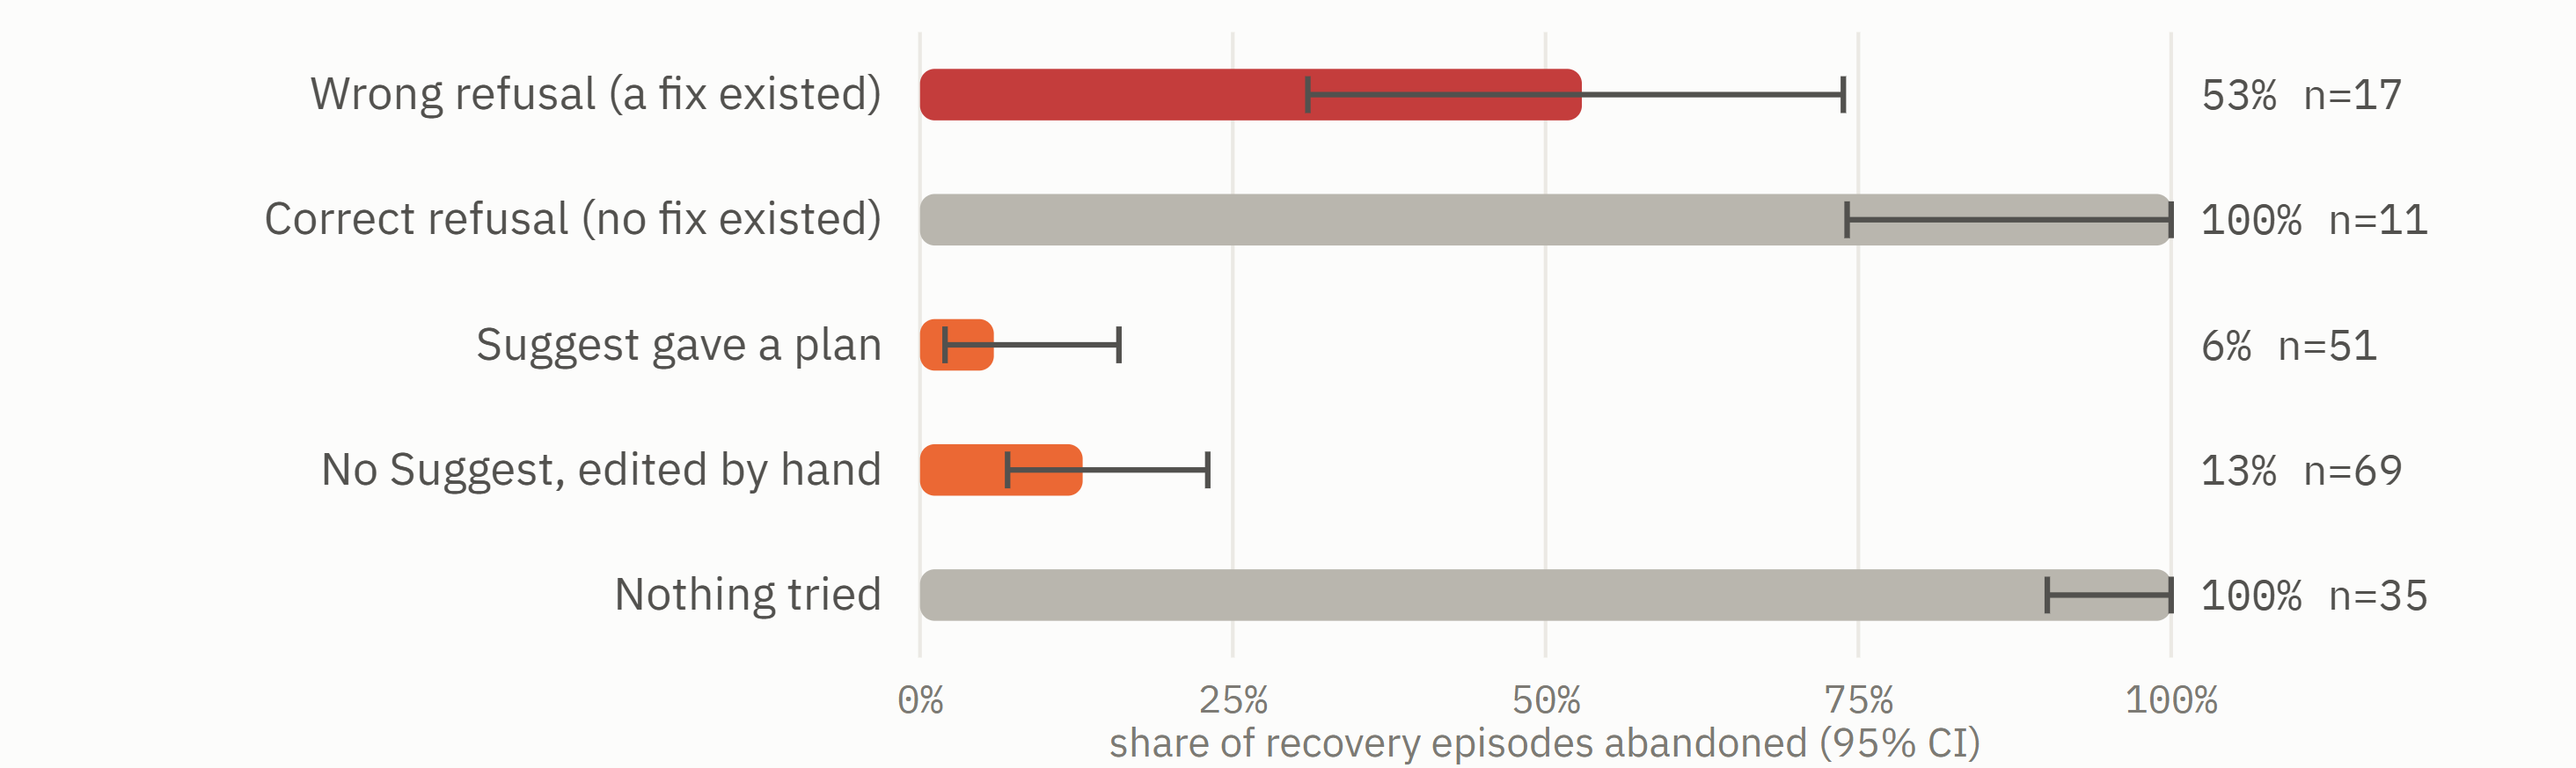
\includegraphics[width=\linewidth,height=0.55\textheight,keepaspectratio]{figs/results/f-flaw-odd__rates__main.png}
\caption{\textbf{Abandonment by what Suggest said}}
\label{fig:res:flaw-odd:rates}
\end{figure}

\paragraph*{Key numbers.}

\begin{itemize}[leftmargin=1.2em,itemsep=1pt]

\item Wrong refusal: 9 of 17 abandoned (53\% [31\%, 74\%]), 14 people; all 17 fixable with drones on the mission

\item Correct refusal: 11 of 11 abandoned (100\% [74\%, 100\%]), 6 people

\item Suggest gave a plan: 3 of 51 (6\%); hand edits only: 9 of 69 (13\%); nothing tried: 35 of 35 (+11 left open)

\item Wrong refusal vs other attempted fixable failures: 9/17 vs 10/118; odds $\times$12.2, Fisher p < .0001; GEE $\times$12.3 [3.2, 47.6], p = .0003

\item The same 14 people on their other attempted fixable failures: 6 of 61 abandoned

\end{itemize}

\paragraph*{Method.} {\small Recovery episodes are rebuilt by h3\_recovery.load\_all (194 episodes, 33 people). It is a time-local rebuild of which drones were on the mission, idle or executing, at each Suggest press. A press is a \textbf{refusal} when Suggest could not cover every task the operator's live plan left short. A refusal is \textbf{wrong} when those tasks could have been covered by drones still on the mission, counting ones busy on another task (chaining them on). Suggest only offers drones that are not executing, which is its blind spot. An episode counts as a wrong refusal if it had at least one wrong-refusal press; as a correct refusal if it had refusals and none was wrong. Rates are abandoned $\div$ (abandoned + recovered), with Wilson 95\% CIs. The comparison counts wrong-refusal episodes against every other fixable episode where something was attempted (Suggest gave a plan, or hand edits): Fisher exact test, plus a GEE logit clustered by person (odds ratio 12 means the odds of abandoning were twelve times higher).}

\clearpage

\subsubsection{Do they check after a refusal? What the log shows between the refusal and the close}\label{sec:res:flaw-odd:checking-after}

\noindent \passtag{extra: may make it in}

\noindent \regtext{The timeline puts every refusal episode on one row, with 0 as the moment Suggest first said no. After a \textbf{wrong} refusal that ended in abandonment, not one operator dragged a drone in the planner. Three pressed Suggest again, got the same answer, and abandoned. None did anything on another mission in between, so they were not called away. 8 of the 9 abandoned within 10 s of the first refusal, at a median 3.8 s after the last one. That is time for a glance, not a re-plan. The 8 who \textbf{did not} take the refusal at its word look completely different: 7 of 8 started dragging drones, took a median 21 s, and saved the mission. After a correct refusal people behaved the same way as after a wrong one (abandoned in a median 4.4 s, no drags). That is right in those cases, and it shows operators get no cue to tell the two apart: the message is the same either way. \par \par The verified case: P19, session 1, M003. Camera-2 failed. The Supply Drop needed a Camera. Two Lifters sat idle, and the only remaining Camera was busy on Search \& Service, due to finish in about 45 s. Suggest said ``No workable plan'', and the operator abandoned 3 s later. Chaining that Camera on would have saved it (checked frame by frame on the recording). P19 later blamed themselves for failed missions (C19). No wrong-refusal abandoner is among the three who blamed the assistant (C20).} (Figure~\ref{fig:res:flaw-odd:checking-after})

\begin{figure}[H]
\centering
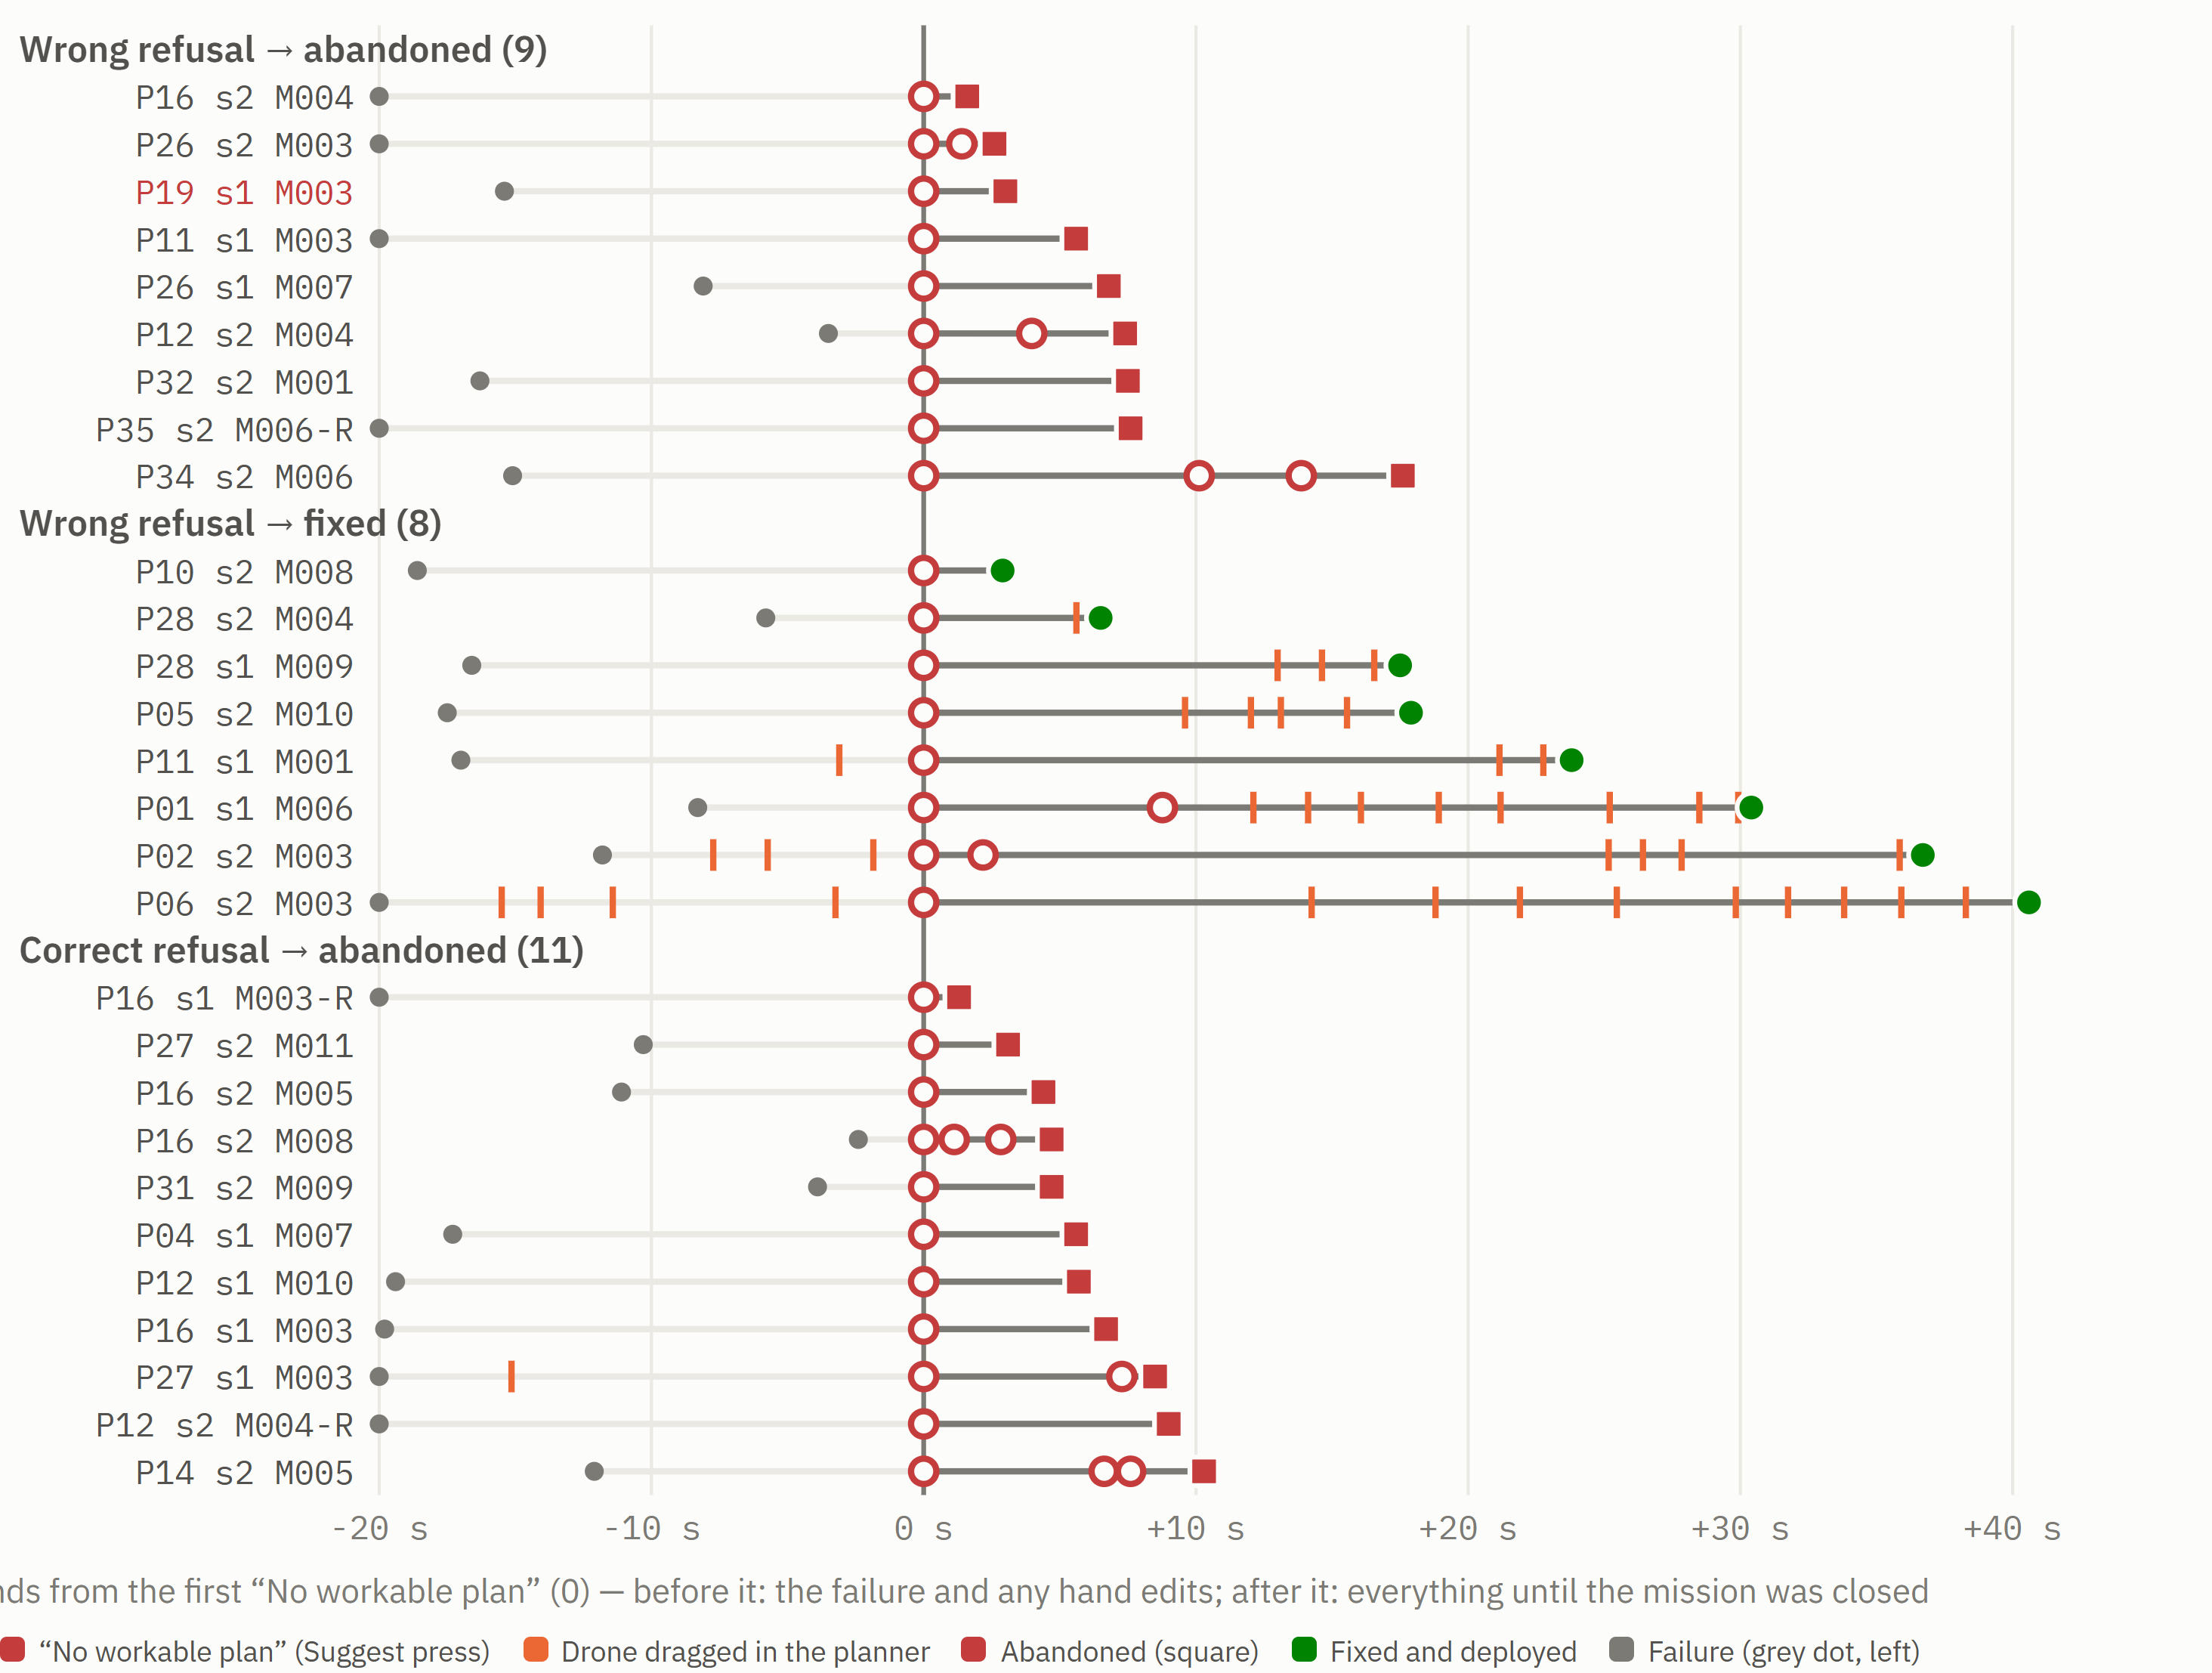
\includegraphics[width=\linewidth,height=0.55\textheight,keepaspectratio]{figs/results/f-flaw-odd__checking-after__main.png}
\caption{\textbf{Do they check after a refusal? What the log shows between the refusal and the close}}
\label{fig:res:flaw-odd:checking-after}
\end{figure}

\paragraph*{Key numbers.}

\begin{itemize}[leftmargin=1.2em,itemsep=1pt]

\item Wrong refusal $\rightarrow$ abandoned (9 episodes, 8 people): drags after the refusal 0 of 9; re-pressed Suggest 3 of 9; actions elsewhere 0 of 9; dragged before the refusal 0 of 9

\item 8 of 9 abandoned within 10 s of the first refusal; median 6.8 s from the first refusal, 3.8 s from the last

\item Wrong refusal $\rightarrow$ fixed (8 episodes, 7 people): 7 of 8 dragged drones after; median 20.9 s to deploy

\item Correct refusal $\rightarrow$ abandoned (11, 6 people): 0 drags after, 3 retries, median 4.4 s from the last refusal

\item Verified: P19 s1 M003, abandoned \textasciitilde{}3 s after the refusal

\end{itemize}

\paragraph*{Method.} {\small For each refusal episode the analysis takes the time of the first refusal and lists every logged operator action from then until the mission was abandoned or redeployed. That includes drags in the recovery planner (tactical\_assignment\_changed), further Suggest presses, and any action on another mission (strategic decisions, tactical confirms, recalls, other recoveries), from the raw event log. ``Checked'' here can only mean a \emph{logged} action. Looking at the strategic map or the planner leaves no trace, so a fast abandonment could still hide a quick look, and the narration recordings are the place to check that. Seconds are session time; the session pauses if the primary window is hidden, so these are real play seconds.}

\clearpage

\subsection{The Tactical Assistant is trusted more, and most people say so too (supplementary analyses)}\label{sec:sup:res:tier-trust}

\noindent Supplement to Section~\ref{sec:res:tier-trust}.

\subsubsection{Is the tactical plan given less attention in Strategic Heavy sessions?}\label{sec:res:tier-trust:attention}

\noindent \passtag{extra: may make it in}

\noindent \regtext{A check of the idea that tactical trust is higher in Strategic Heavy sessions because the tactical plan gets less attention there. Raw, it does: in Strategic Heavy sessions people press Suggest less, edit less and spend less time in the planner. But Strategic Heavy plans are much smaller (5.3 vs 8.1 drones). Compared at the same plan size and session order, the planner is open about 12\% less long and the checking is about 9\% shorter, but neither is distinguishable from no difference, and editing is the same. The one clear difference is the other way round: on same-size plans people press Suggest \emph{more} in Strategic Heavy (odds $\times$1.5). People whose planner time drops more do not clearly trust the Tactical Assistant more ($\rho$ = $-$.24, p = .19). And tactical trust itself barely differs between the scenarios (+0.15, p = .25); the gap comes from strategic trust. So the attention account is not supported, though a small effect cannot be ruled out.} (Figure~\ref{fig:res:tier-trust:attention})

\begin{figure}[H]
\centering
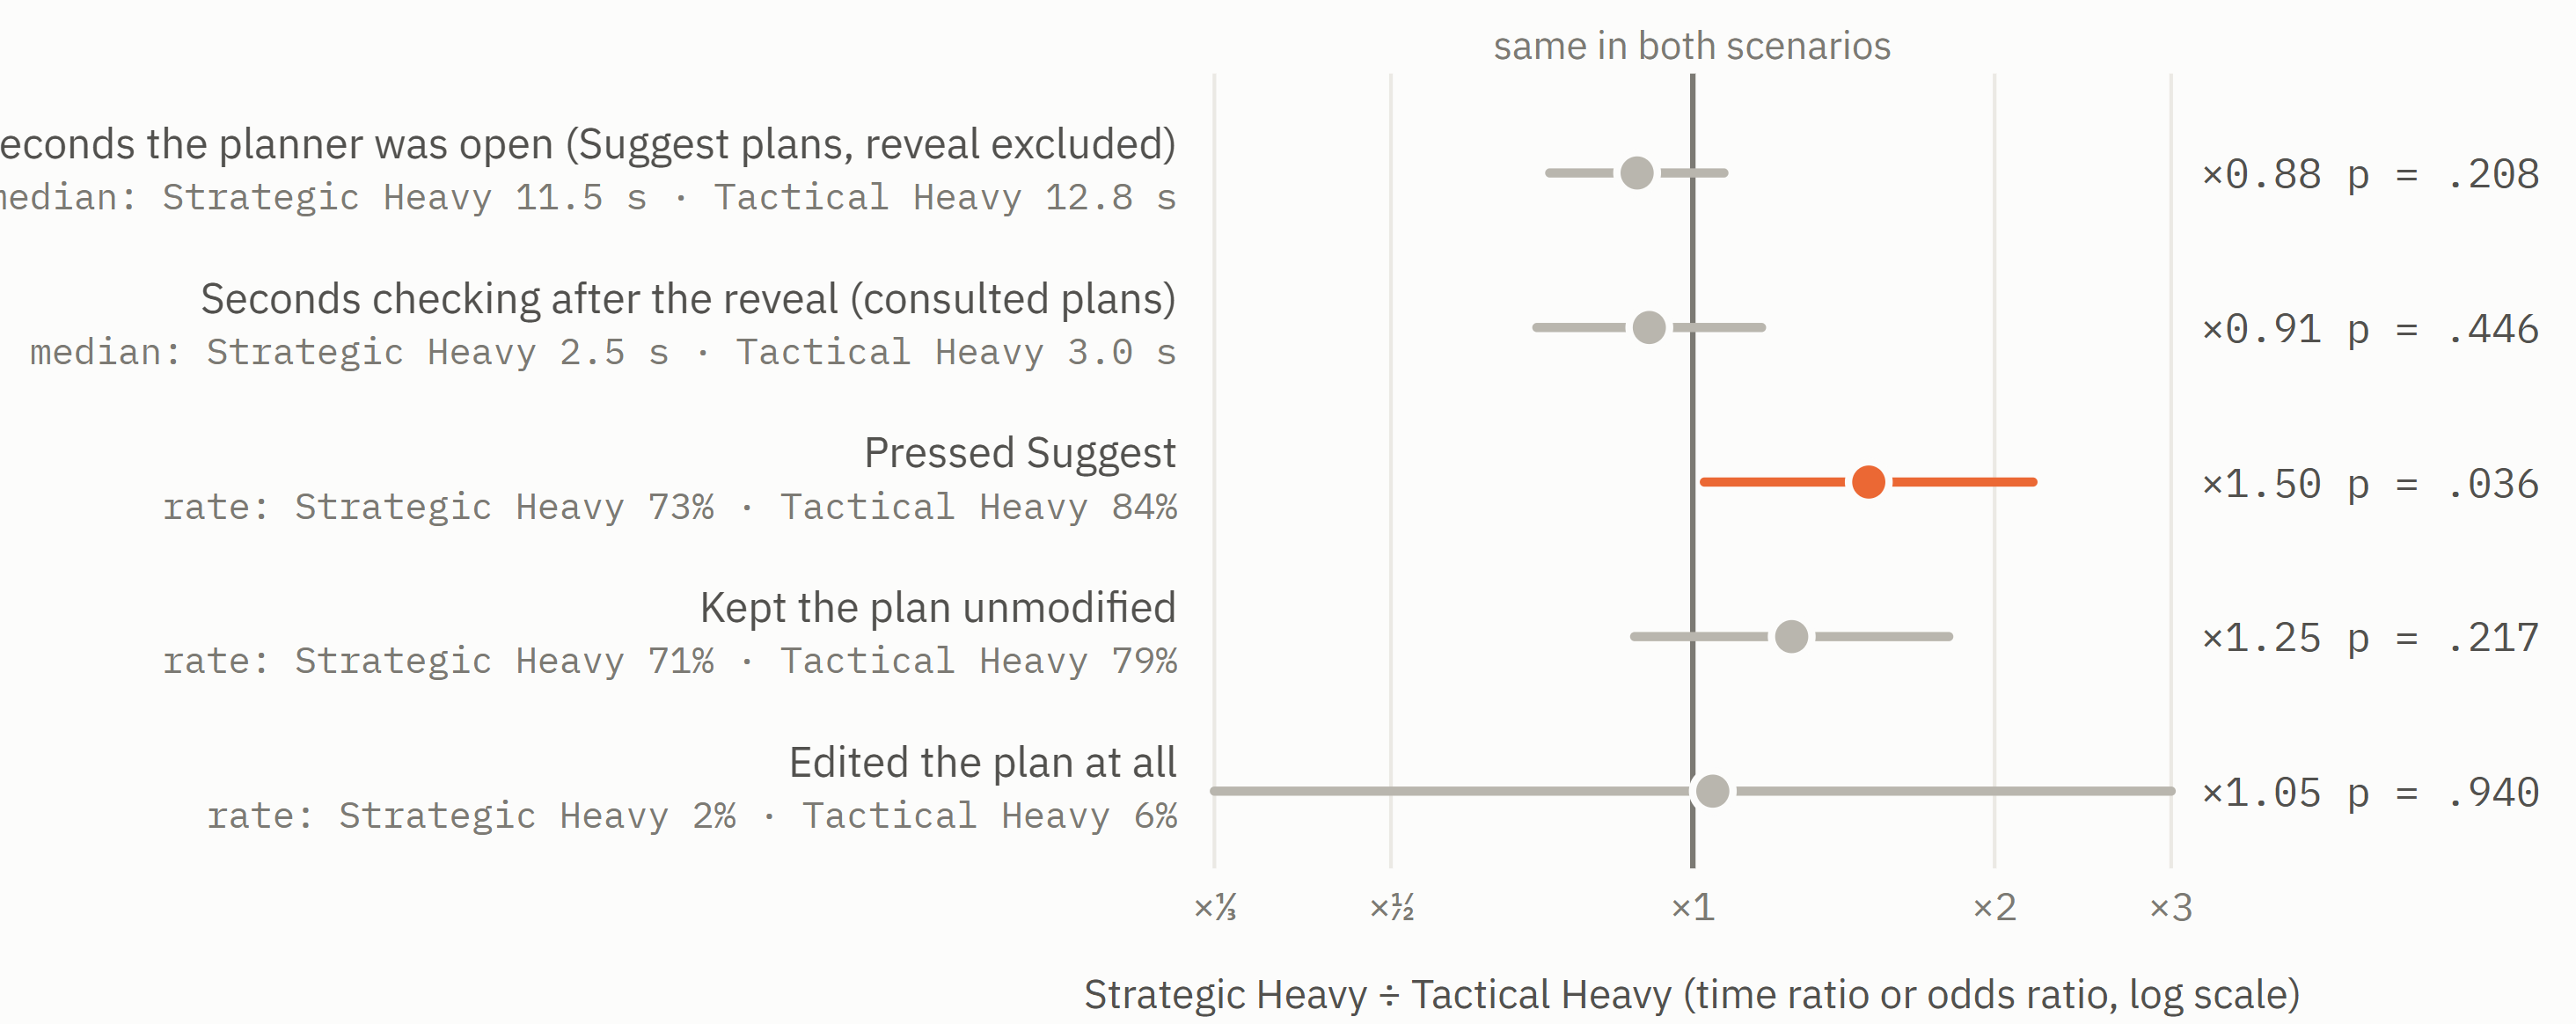
\includegraphics[width=\linewidth,height=0.55\textheight,keepaspectratio]{figs/results/f-tier-trust__attention__main.png}
\caption{\textbf{Is the tactical plan given less attention in Strategic Heavy sessions?}}
\label{fig:res:tier-trust:attention}
\end{figure}

\paragraph*{Key numbers.}

\begin{itemize}[leftmargin=1.2em,itemsep=1pt]

\item Planner time (Suggest plans): median 11.5 s Strategic Heavy vs 12.8 s Tactical Heavy; adjusted $\times$0.88 [0.72, 1.07], p = .21

\item Checking time after the reveal: median 2.5 s vs 3.0 s; adjusted $\times$0.91 [0.70, 1.17], p = .45

\item Suggest pressed: 73\% vs 84\% raw (OR 0.56, p = .005); same-size plans OR 1.50 [1.03, 2.18], p = .036

\item Kept unmodified: 71\% vs 79\% raw (OR 0.67, p = .046); adjusted OR 1.26 [0.88, 1.80], p = .22

\item Edited at all: 2\% vs 6\% raw (OR 0.44, p = .033); adjusted OR 1.05 [0.32, 3.47], p = .94

\item Attention drop vs tactical-trust rise, person by person: $\rho$ = $-$.24 [$-$.56, .12], p = .19, n = 31

\end{itemize}

\paragraph*{Method.} {\small 630 tactical plans, 33 people (P09 excluded): 381 in Strategic Heavy sessions, 249 in Tactical Heavy. Five measures per plan. \textbf{Planner time}: from the planner opening to Deploy, minus the forced one-second-per-pair reveal, on plans where Suggest was pressed (486), so it is time spent with the assistant's plan. \textbf{Checking time}: last Suggest press to Deploy, minus the reveal (the ``checking'' measure of the section above). \textbf{Suggest pressed}, \textbf{kept unmodified} and \textbf{edited at all} on every plan. Each is compared Strategic Heavy vs Tactical Heavy with a GEE model clustered by person: times on the log scale (so the result is a ratio of typical seconds), yes/no measures as odds ratios. \textbf{Raw} has scenario only; \textbf{adjusted} adds plan size (drones $\times$ tasks) and session order, so it compares like-for-like plans. The trust link: each person's average size-and-session-adjusted log planner time in each scenario, the Strategic Heavy minus Tactical Heavy difference, against their difference in tactical trust; Spearman $\rho$ with a bootstrap 95\% CI (31 people with Suggest plans in both scenarios).}

\clearpage

\subsubsection{A bad first session with the cards does not explain who loses strategic trust}\label{sec:res:tier-trust:own-failures}

\noindent \passtag{numbers only}

\noindent \regtext{If strategic trust fell because people had bad experiences with the cards, then those who met more illogical cards in session 1 should lose more trust. They do not. The raw correlation even points the other way ($\rho$ = +.40), but that comes entirely from scenario order: people who played Strategic Heavy first see the odd cards early and lose the least trust ($-$0.29 against $-$1.26 for those who played it second). Once order is held constant, the correlation is +.14 (p = .42). Round 1's pre-registered version (missions that failed after a card) was also null: $\rho$ = $-$.05 [$-$.39, .30]. Read this as ``no evidence that how much went wrong drives it'', not as proof that experience doesn't matter.}

\paragraph*{Key numbers.}

\begin{itemize}[leftmargin=1.2em,itemsep=1pt]

\item Illogical cards seen in session 1 vs change in strategic trust: $\rho$ = +.40 [+.03, +.70], p = .02 --- order artefact

\item Same, holding scenario order fixed: $\rho$ = +.14, p = .42

\item Mean change in strategic trust $-$0.76; Strategic Heavy first $-$0.29, Tactical Heavy first $-$1.26

\item H5 primary (card failures in session 1): $\rho$ = $-$.05 [$-$.39, .30]

\end{itemize}

\paragraph*{Method.} {\small One row per person (33). The predictor is the count of decisions in session 1 where an illogical strategy card was on screen (from load\_decisions' odd flag). The outcome is session-2 minus session-1 strategic trust. Spearman $\rho$ uses a 4000-draw seeded bootstrap CI. The partial version ranks both variables, removes the part explained by which scenario was played first, and correlates what is left. The $\rho$ = $-$.05 is H5's primary test (docs/analysis/round1/h5\_trust\_drop.md).}

\clearpage

\subsubsection{What they said agrees with what they rated}\label{sec:res:tier-trust:stated}

\noindent \passtag{numbers only}

\noindent \regtext{In the debriefs and interviews, 17 operators named the Tactical Assistant as the one they preferred or trusted, 7 the Strategic one, and 9 gave a conditional, ``both'' or no answer. Those who said tactical had a questionnaire gap of +1.36 on average; those who said strategic were at $-$0.04. For 18 of the 24 who named one side, the questionnaire points the same way. The coding is from one coder (an AI model) and has not been second-coded, so treat the counts as suggestive.} (Figure~\ref{fig:res:tier-trust:stated})

\begin{figure}[H]
\centering
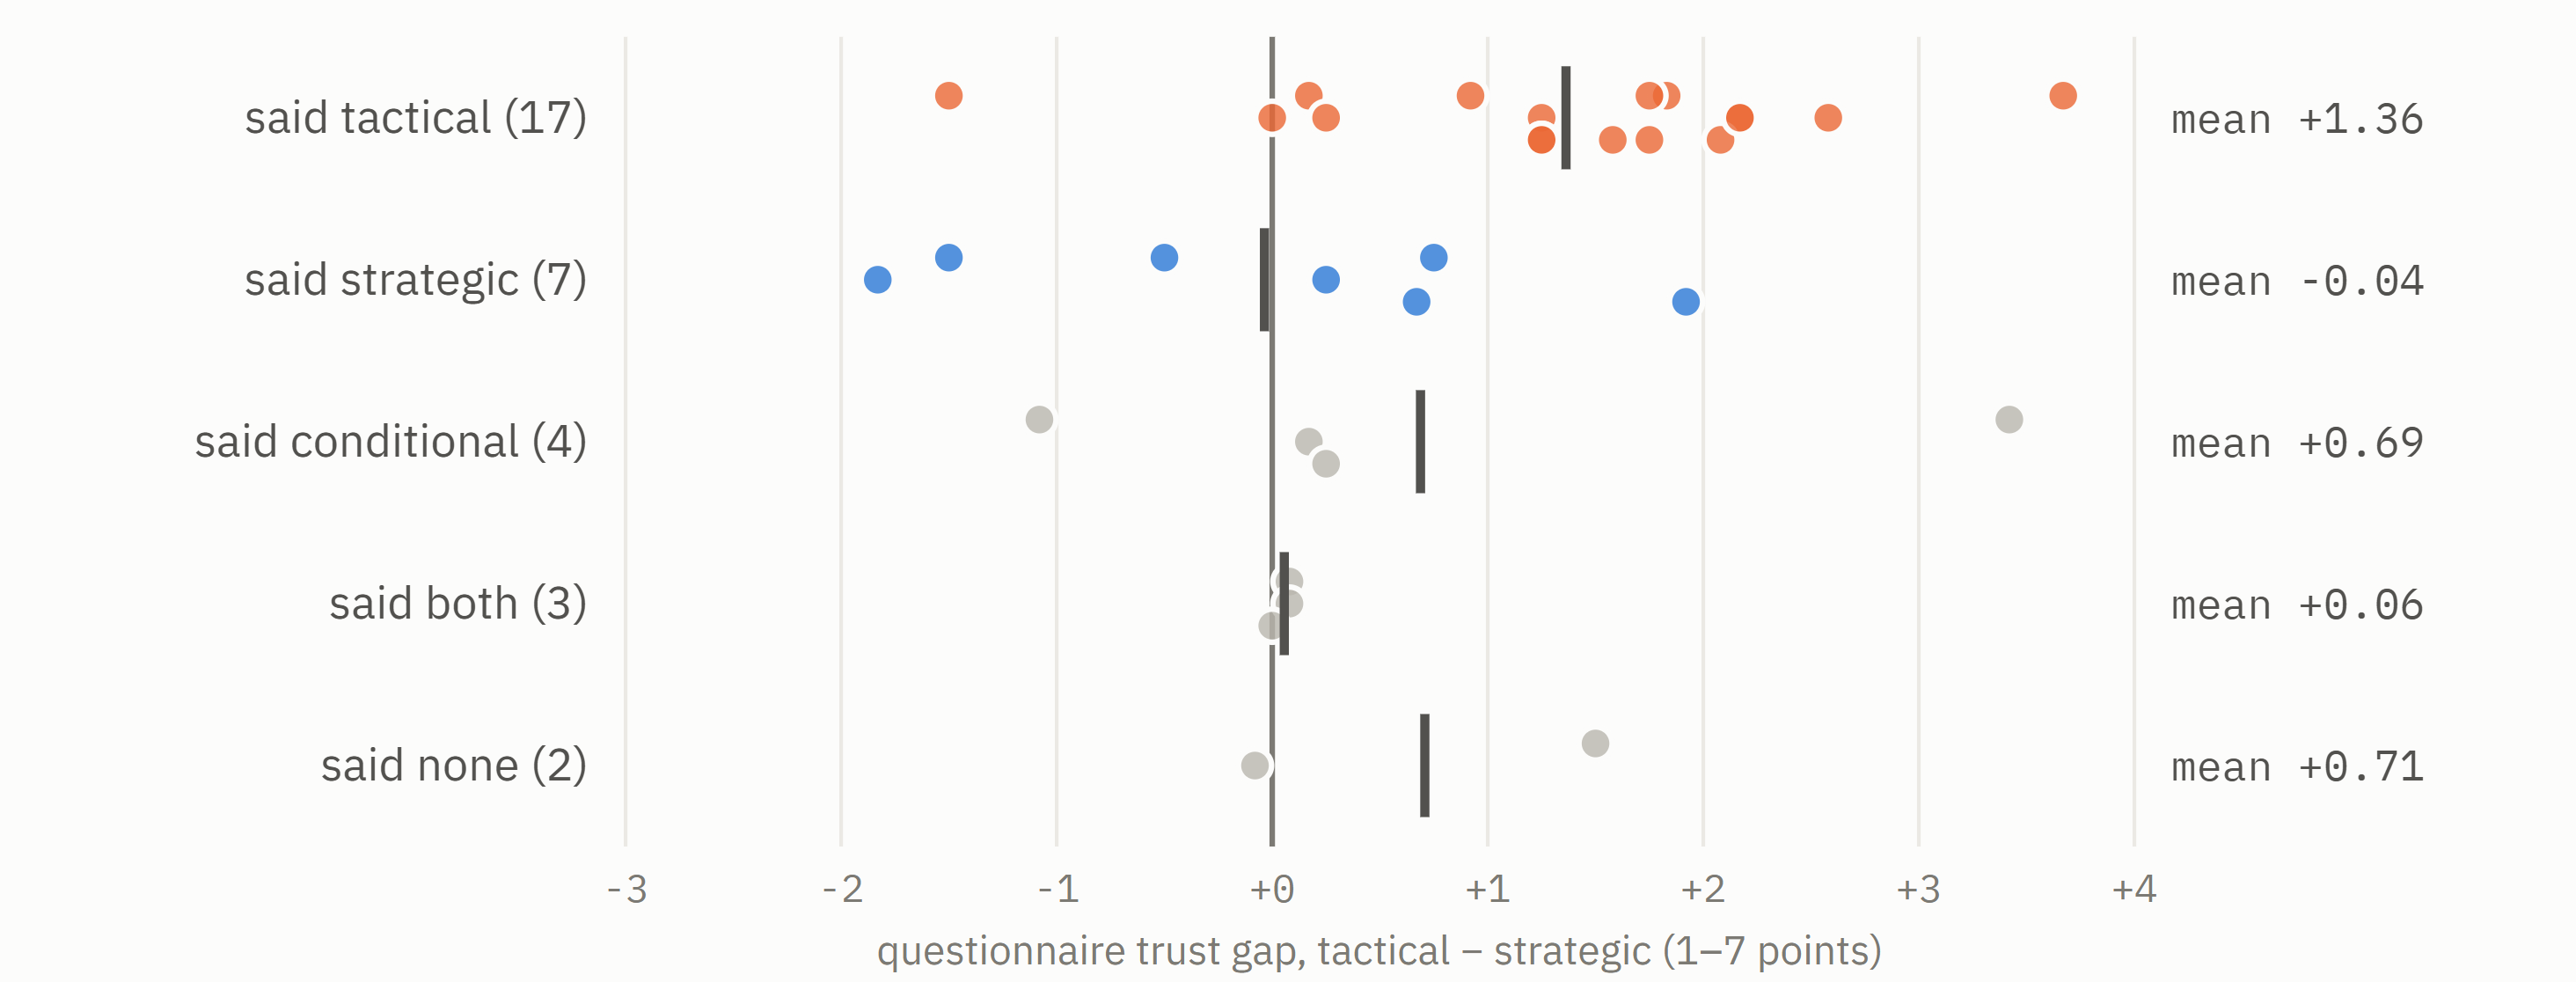
\includegraphics[width=\linewidth,height=0.55\textheight,keepaspectratio]{figs/results/f-tier-trust__stated__main.png}
\caption{\textbf{What they said agrees with what they rated}}
\label{fig:res:tier-trust:stated}
\end{figure}

\paragraph*{Key numbers.}

\begin{itemize}[leftmargin=1.2em,itemsep=1pt]

\item Said tactical 17, strategic 7, conditional 4, both 3, none 2

\item Sign test 17 of 24: p = .064

\item Questionnaire gap: tactical-sayers +1.36 [+0.76, +1.97] vs strategic-sayers $-$0.04 [$-$1.27, +1.19]; Mann--Whitney p = .033

\item Questionnaire agrees with the stated side for 18 of 24

\end{itemize}

\paragraph*{Method.} {\small Stated preference is the round-2 coding of each person's debrief and interview (docs/analysis/round2/wE\_codes.csv, field pref). Its sign test asks whether 17 of 24 is more lopsided than a coin toss (exact binomial, two-sided, p = .064). The other test compares the questionnaire gap of tactical-sayers with strategic-sayers (Mann--Whitney, p = .033). Round 1's independent coding agreed poorly with it ($\kappa$ = .27), and round 2's $\kappa$ = .96 came from the same AI model. A human second coder is still needed (meth-qual-coder).}

\clearpage

\subsection{A practitioner's reading: P36, a participant with operational military experience (supplementary analyses)}\label{sec:sup:qual:practitioner}

\noindent Supplement to Section~\ref{sec:qual:practitioner}.

\subsubsection{Passages not picked this pass}\label{sec:qual:practitioner:not-picked}

\noindent \regtext{The passages from the same participant that were not picked for the main section, kept so nothing is lost. Each carries the links back it was first given; they were not re-read against a trimmed version.}

\clearpage
